% Options for packages loaded elsewhere
\PassOptionsToPackage{unicode}{hyperref}
\PassOptionsToPackage{hyphens}{url}
\documentclass[
  10pt,
]{article}
\usepackage{xcolor}
\usepackage[margin=0.85in]{geometry}
\usepackage{amsmath,amssymb}
\setcounter{secnumdepth}{5}
\usepackage{iftex}
\ifPDFTeX
  \usepackage[T1]{fontenc}
  \usepackage[utf8]{inputenc}
  \usepackage{textcomp} % provide euro and other symbols
\else % if luatex or xetex
  \usepackage{unicode-math} % this also loads fontspec
  \defaultfontfeatures{Scale=MatchLowercase}
  \defaultfontfeatures[\rmfamily]{Ligatures=TeX,Scale=1}
\fi
\usepackage{lmodern}
\ifPDFTeX\else
  % xetex/luatex font selection
\fi
% Use upquote if available, for straight quotes in verbatim environments
\IfFileExists{upquote.sty}{\usepackage{upquote}}{}
\IfFileExists{microtype.sty}{% use microtype if available
  \usepackage[]{microtype}
  \UseMicrotypeSet[protrusion]{basicmath} % disable protrusion for tt fonts
}{}
\makeatletter
\@ifundefined{KOMAClassName}{% if non-KOMA class
  \IfFileExists{parskip.sty}{%
    \usepackage{parskip}
  }{% else
    \setlength{\parindent}{0pt}
    \setlength{\parskip}{6pt plus 2pt minus 1pt}}
}{% if KOMA class
  \KOMAoptions{parskip=half}}
\makeatother
\usepackage{graphicx}
\makeatletter
\newsavebox\pandoc@box
\newcommand*\pandocbounded[1]{% scales image to fit in text height/width
  \sbox\pandoc@box{#1}%
  \Gscale@div\@tempa{\textheight}{\dimexpr\ht\pandoc@box+\dp\pandoc@box\relax}%
  \Gscale@div\@tempb{\linewidth}{\wd\pandoc@box}%
  \ifdim\@tempb\p@<\@tempa\p@\let\@tempa\@tempb\fi% select the smaller of both
  \ifdim\@tempa\p@<\p@\scalebox{\@tempa}{\usebox\pandoc@box}%
  \else\usebox{\pandoc@box}%
  \fi%
}
% Set default figure placement to htbp
\def\fps@figure{htbp}
\makeatother
\setlength{\emergencystretch}{3em} % prevent overfull lines
\providecommand{\tightlist}{%
  \setlength{\itemsep}{0pt}\setlength{\parskip}{0pt}}
\usepackage{booktabs}
\usepackage{longtable}
\usepackage{array}
\usepackage{multirow}
\usepackage{wrapfig}
\usepackage{float}
\usepackage{colortbl}
\usepackage{pdflscape}
\usepackage{tabularx}
\usepackage{xltabular}
\usepackage{threeparttable}
\usepackage{threeparttablex}
\usepackage[normalem]{ulem}
\usepackage{makecell}
\usepackage{xcolor}
\usepackage{bookmark}
\IfFileExists{xurl.sty}{\usepackage{xurl}}{} % add URL line breaks if available
\urlstyle{same}
% fallback for those not using the hyperref driver hyperxmp:
\makeatletter
\@ifundefined{xmpquote}{\newcommand{\xmpquote}[1]{#1}}{}
\makeatother
\hypersetup{
  pdftitle={Comparative Evaluation of Four DIA Proteomics Pipelines},
  pdfauthor={Mohieddin Jafari},
  hidelinks,
  pdfcreator={LaTeX via pandoc}}

\title{Comparative Evaluation of Four DIA Proteomics Pipelines}
\usepackage{etoolbox}
\makeatletter
\providecommand{\subtitle}[1]{% add subtitle to \maketitle
  \apptocmd{\@title}{\par {\large #1 \par}}{}{}
}
\makeatother
\subtitle{Capstone Project 2026}
\author{Mohieddin Jafari}
\date{2026-11-10}

\begin{document}
\maketitle

{
\setcounter{tocdepth}{2}
\tableofcontents
}
\section{Resources}\label{resources}

\begin{verbatim}
## R version: R version 4.6.0 (2026-04-24)
\end{verbatim}

\begin{verbatim}
## Platform: aarch64-apple-darwin23
\end{verbatim}

\begin{verbatim}
## Operating system: Darwin
\end{verbatim}

\begin{verbatim}
## Report generated: 2026-11-10 14:38:04
\end{verbatim}

\begin{longtable}[t]{ll}
\caption{\label{tab:session_information}R package versions used in the analysis}\\
\toprule
Package & Version\\
\midrule
QFeatures & 1.22.0\\
dplyr & 1.2.1\\
tidyr & 1.3.2\\
ggplot2 & 4.0.3\\
msqrob2 & 1.20.0\\
\addlinespace
stringr & 1.6.0\\
ExploreModelMatrix & 1.24.0\\
MsCoreUtils & 1.24.0\\
matrixStats & 1.5.0\\
patchwork & 1.3.2\\
\addlinespace
kableExtra & 1.4.1\\
ComplexHeatmap & 2.28.0\\
purrr & 1.2.2\\
tibble & 3.3.1\\
scater & 1.40.2\\
\addlinespace
arrow & 26.0.0\\
ggcorrplot & 0.3.0\\
readr & 2.2.0\\
knitr & 1.52\\
rmarkdown & 2.32\\
\addlinespace
bipartite & 2.24\\
\bottomrule
\end{longtable}

\section{Data}\label{data}

\subsection{First time}\label{first-time}

\subsection{Recovery}\label{recovery}

\subsection{Inspect the imported
datasets}\label{inspect-the-imported-datasets}

\subsection{Hemogenize datasets}\label{hemogenize-datasets}

Each row in the precursor data table is in ``long format'' and contains
information about one precursor in a specific run.

\subsection{Select relevant columns for each
software}\label{select-relevant-columns-for-each-software}

Then, we filter the data to reduce the memory footprint.

The sample annotation table is not available and can be generated from
the run labels, as the researchers included information on the design in
the filenames.

\subsection{Qfeatures}\label{qfeatures}

Here, Precursor.Quantity provides the quantitative values, and
Precursor.Id identifies the precursor features.

\subsubsection{1. Recovery qfs}\label{recovery-qfs}

\begin{verbatim}
## [1] TRUE TRUE TRUE TRUE
\end{verbatim}

\begin{verbatim}
## An instance of class QFeatures (type: bulk) with 84 sets:
## 
##  [1] 20260331_c-jun_KO_cDDP_24h1_1: SummarizedExperiment with 324817 rows and 1 columns 
##  [2] 20260331_c-jun_KO_cDDP_24h1_2: SummarizedExperiment with 324817 rows and 1 columns 
##  [3] 20260331_c-jun_KO_cDDP_24h1_3: SummarizedExperiment with 324817 rows and 1 columns 
##  ...
##  [82] Group4_CTRL_JNK-IN-8_cDDP_06h_1: SummarizedExperiment with 324817 rows and 1 columns 
##  [83] Group4_CTRL_JNK-IN-8_cDDP_06h_2: SummarizedExperiment with 324817 rows and 1 columns 
##  [84] Group4_CTRL_JNK-IN-8_cDDP_06h_3: SummarizedExperiment with 324817 rows and 1 columns
\end{verbatim}

\begin{verbatim}
## [1] "20260331_c-jun_KO_cDDP_24h1_1" "20260331_c-jun_KO_cDDP_24h1_2"
## [3] "20260331_c-jun_KO_cDDP_24h1_3" "20260331_c-jun_KO_cDDP_24h2_1"
## [5] "20260331_c-jun_KO_cDDP_24h2_2" "20260331_c-jun_KO_cDDP_24h2_3"
\end{verbatim}

\begin{verbatim}
## [1] 84
\end{verbatim}

\begin{verbatim}
## [[1]]
## [1] 324817      1
## 
## [[2]]
## [1] 324817      1
## 
## [[3]]
## [1] 324817      1
## 
## [[4]]
## [1] 324817      1
## 
## [[5]]
## [1] 324817      1
\end{verbatim}

\begin{verbatim}
##            used  (Mb) gc trigger   (Mb) limit (Mb)  max used   (Mb)
## Ncells  9780270 522.4   18018267  962.3         NA  13497694  720.9
## Vcells 17634954 134.6  194729561 1485.7      24576 224423520 1712.3
\end{verbatim}

\begin{verbatim}
## Recovered experimental design: 84 runs
\end{verbatim}

\begin{verbatim}
##                             Run   condition    Batch
## 1 20260331_c-jun_KO_cDDP_24h1_1 KO_cDDP_24h 20260331
## 2 20260331_c-jun_KO_cDDP_24h1_2 KO_cDDP_24h 20260331
## 3 20260331_c-jun_KO_cDDP_24h1_3 KO_cDDP_24h 20260331
\end{verbatim}

\section{Data preprocessing}\label{data-preprocessing}

The data preprocessing workflow for DIA data is similar to the workflow
for DDA-LFQ data, but there are suble differences as we start from
precursor level data and have additional columns.

\subsection{Missing values}\label{missing-values}

The first preprocessing step is to correctly encode the missing values.
It is important that missing values are encoded using \texttt{NA}. For
instance, non-observed values should not be encoded with a zero because
true zeros (the proteomic feature is absent from the sample) cannot be
distinguished from technical zeros (the feature was missed by the
instrument or could not be identified). We therefore replace any zero in
the quantitative data with an \texttt{NA}.

Inspection of the precursor-level QFeatures objects revealed differences
in how missing measurements are represented across the four DIA software
packages. AlphaDIA contained 324,817 precursor entries in each of the 84
runs, with 13,010,298 intensity values encoded as zeros. DIA-NN and
Spectronaut already represented missing intensity measurements as NA,
with 10,497,983 and 49 missing values, respectively, in the QFeatures
objects. In contrast, MaxDIA contained 15,350,731 precursor observations
across 84 runs, with varying numbers of precursor entries per run and no
explicit zeros or NA values. These differences indicate that AlphaDIA
represents unquantified precursor measurements as zeros, DIA-NN and
Spectronaut use explicit NA values for missing measurements, and MaxDIA
reports only available precursor records. However, the absence of
explicit missing values does not imply complete precursor coverage
across runs, as unreported precursor--run combinations may be absent
from the individual assays. Therefore, AlphaDIA's zero intensities will
be converted to NA using zeroIsNA(), while missing precursor--run
combinations will be accounted for when aligning precursor identifiers
across runs.

\subsection{Joining assay}\label{joining-assay}

Combine 84 run-specific assays into one precursor assay for each DIA
software:

\subsubsection{2. Recovery qfs}\label{recovery-qfs-1}

\begin{verbatim}
## [1] TRUE TRUE TRUE TRUE
\end{verbatim}

\subsection{Filtering}\label{filtering}

Precursor-level filtering was performed independently for AlphaDIA,
DIA-NN, Spectronaut, and MaxDIA. Precursors were retained if they had
positive, non-missing intensities in at least two-thirds of the samples
within any one experimental condition, preserving condition-specific
signals. Annotated decoys, reverse hits, and potential contaminants were
excluded. Proteotypic filtering was applied using DIA-NN's explicit
annotation and a single-protein-identifier criterion for MaxDIA;
however, proteotypic status could not be reliably verified for AlphaDIA
and Spectronaut, so these precursors were retained pending further
assessment. No minimum peptide count per protein was imposed. Following
filtering, AlphaDIA retained 62.5\%, DIA-NN 67.8\%, Spectronaut 90.8\%,
and MaxDIA 63.6\% of their initial precursors. Spectronaut's higher
retention reflects its nearly complete quantitative matrix, whereas
detection-frequency filtering had a greater impact on the other
pipelines. Differences in software-specific quantification and
proteotypic annotations should therefore be considered when interpreting
precursor coverage.

\subsection{Log-transformation}\label{log-transformation}

Following precursor-level filtering, intensity values were
log2-transformed using the \texttt{logTransform()} function from the
QFeatures package to reduce right-skewness and improve comparability of
quantitative measurements. The transformed intensities were stored in a
new assay named precursors\_log, while the original filtered intensities
were preserved in precursors. Both assays were retained within each
software-specific QFeatures object (\texttt{qf\_alpha},
\texttt{qf\_diann}, \texttt{qf\_spectro}, and \texttt{qf\_maxdia}),
maintaining their metadata and processing relationships for subsequent
analysis.

Unlike the other three software packages, Spectronaut has a distinctly
multimodal intensity distribution, including a sharp peak near log2
intensity = 0 and a broader low-intensity population between
approximately 2 and 7. This is particularly suspicious because almost
every Spectronaut precursor has a reported intensity in all 84 runs,
despite IsImputed = False throughout. \#\#\# Extra filtering step

Run chunk 23 to re-visualize the distribution after extra filtering.

\subsection{Normalization}\label{normalization}

Systematic technical variation between LC-MS runs can introduce
differences in measured precursor intensities that are unrelated to
biological conditions. Pre-normalization QC revealed batch-associated
intensity shifts across the four DIA analysis pipelines. To account for
run-level differences, the Median of Ratios method was applied
independently to each software's log2-transformed precursor intensities.
Normalization factors were calculated using
\texttt{nfLogMedianOfRatios()} and subtracted from each corresponding
run using \texttt{sweep()}. The normalized intensities were stored in a
new assay named \texttt{precursors\_norm}, preserving the original
precursors and \texttt{precursors\_log} assays.

\subsubsection{Removing outlier run}\label{removing-outlier-run}

One LC-MS run (Group1\_c-jun\_KO\_1) exhibited an atypical precursor
intensity distribution across multiple DIA analysis pipelines, most
prominently in AlphaDIA and DIA-NN. Given the consistency of this
observation across software tools and the availability of additional
replicates for the corresponding condition, the run was excluded from
downstream quantitative analysis. Normalization was subsequently
recalculated using the remaining 83 runs.

The results strengthen the justification for excluding
Group1\_c-jun\_KO\_1, particularly for DIA-NN and MaxDIA (Run chunk 26
to re-check).

\subsection{NIMAA analysis of precursor
detection}\label{nimaa-analysis-of-precursor-detection}

Precursor detection was represented as a binary precursor-by-run matrix
(observed = 1; missing = 0). The NIMAA-style
\texttt{Rectangular\_element\_max} method was applied to all precursor
features to identify a fully observed rectangular submatrix. The
efficient implementation was checked against the original NIMAA output
on a 5,000-precursor test matrix.

\begin{verbatim}
## Successfully recovered normalized QFeatures for all four pipelines.
\end{verbatim}

\begin{verbatim}
##     Software Precursors Runs Observed_pct Missing_pct Complete_precursors
##     AlphaDIA     203024   83        73.48       26.52               39666
##       DIA-NN     206959   83        76.00       24.00               45613
##  Spectronaut     182083   83        93.73        6.27               75295
##       MaxDIA     230167   83        68.81       31.19               22251
##  Complete_runs
##              0
##              0
##              0
##              0
\end{verbatim}

Spectronaut had the largest complete submatrix (6.25 million cells;
41.35\% of its original matrix), including all 83 runs. DIA-NN included
the greatest proportion of original precursors (45.66\%) but only 42
runs. AlphaDIA included 81 runs and 20.14\% of original matrix cells;
MaxDIA included 58 runs and 12.45\%.

Nestedness temperature was estimated using 5,000 randomly sampled
precursors per pipeline, with all 83 runs. Spectronaut had the lowest
temperature (6.96), followed by DIA-NN (17.71), AlphaDIA (23.78), and
MaxDIA (28.50). Lower values indicate more nested detection patterns.
Overall, Spectronaut showed the most complete and nested detection
structure in this analysis. Differences in precursor sets and matrix
fill limit direct interpretation of nestedness as quantitative
performance.

Repeated sampling (20 iterations of 5,000 precursors) showed consistent
differences in nestedness temperature across pipelines. Spectronaut had
the lowest mean temperature (6.84 ± 0.22), followed by DIA-NN (18.08 ±
0.33), AlphaDIA (23.49 ± 0.35), and MaxDIA (28.50 ± 0.42). The low
variability across repetitions indicates stable estimates under the
sampling procedure, with Spectronaut exhibiting the most strongly nested
precursor detection pattern. \#\# Aggregation The objective of
aggregation is to summarise the precursor-level intensities into a
protein expression value. The fact that different precursors have
different intensities (2.), may be inconsistently identified (3.) and/or
quantified (4.), and show sample correlations (5.) can lead to bias if
we use simple summarisation approaches such as summing or averaging the
precursor intensities for each sample. Instead, we will resort to more
advanced summarisation approaches to accommodate for these issues. Here,
we summarise the precursor-level data into protein intensities
usin\texttt{g\ maxLFQ}. It is implemented in the \texttt{maxLFQ}
function of the \texttt{iq} package.

\subsubsection{3. Recovery qfs}\label{recovery-qfs-2}

\begin{verbatim}
##      Software                                                Assays
## 1    AlphaDIA precursors, precursors_log, precursors_norm, proteins
## 2       DIANN precursors, precursors_log, precursors_norm, proteins
## 3 Spectronaut precursors, precursors_log, precursors_norm, proteins
## 4      MaxDIA precursors, precursors_log, precursors_norm, proteins
##   Protein_Assay Proteins Runs
## 1          TRUE    11331   83
## 2          TRUE     9833   83
## 3          TRUE     7970   83
## 4          TRUE     8482   83
\end{verbatim}

The tutorial uses longForm() to visualize every measurement. Because
your datasets are large, this version samples up to 2,000 quantified
proteins per run for plotting, while retaining all protein measurements
in the QFeatures objects.

Overall, MaxLFQ aggregation produced reasonably consistent protein-level
intensity distributions across the 83 runs in all four software
packages. - AlphaDIA: Narrow, closely overlapping distributions,
indicating good run-to-run consistency. - DIA-NN: Broader distributions
with slightly more variability, but generally good overlap. -
Spectronaut: Strong overlap around the main peak, although a small
low-intensity tail remains. - MaxDIA: Good overall alignment, with some
variability in peak height and distribution shape.

The protein-level distributions look suitable for proceeding to
downstream QC and differential abundance analysis. There are no obvious
extreme run-level outliers remaining.

The data processing is complete.

\section{Data exploration and QC}\label{data-exploration-and-qc}

Data exploration aims to highlight the main sources of variation in the
data prior to data modelling and can pinpoint to outlying or
off-behaving samples.

\subsection{NIMAA analysis of
proteins}\label{nimaa-analysis-of-proteins}

\begin{verbatim}
##     Software Proteins Runs Observed_pct Missing_pct Complete_proteins
##     AlphaDIA    11331   83        96.44        3.56              8828
##       DIA-NN     9833   83        95.07        4.93              7557
##  Spectronaut     7970   83        99.68        0.32              7581
##       MaxDIA     8482   83        99.36        0.64              7515
\end{verbatim}

Protein-level NIMAA analysis showed substantially higher completeness
than precursor-level analysis across all four DIA pipelines.
\textbf{AlphaDIA} produced the largest complete submatrix (8,937
proteins × 82 runs; 77.92\% matrix coverage), whereas
\textbf{Spectronaut} achieved the highest proportional coverage
(95.12\%), followed by MaxDIA (88.60\%), DIA-NN (76.85\%), and AlphaDIA
(77.92\%).

Nestedness temperatures calculated using \textbf{all proteins and 83
runs} were lowest for MaxDIA (0.022) and Spectronaut (0.026), followed
by AlphaDIA (1.150) and DIA-NN (1.448). These low values indicate highly
nested protein detection patterns.

Overall, protein aggregation substantially reduced missingness, allowing
nearly all runs to be preserved in complete submatrices. Spectronaut and
MaxDIA exhibited the most complete and strongly nested protein-level
detection patterns, while AlphaDIA provided the largest absolute number
of complete protein measurements. These findings reflect detection
completeness rather than quantitative accuracy.

\subsection{Normalized precursor intensity density
plots}\label{normalized-precursor-intensity-density-plots}

\begin{verbatim}
##             used   (Mb) gc trigger   (Mb) limit (Mb)  max used   (Mb)
## Ncells  12121821  647.4   18018267  962.3         NA  17963417  959.4
## Vcells 549662682 4193.6  854737090 6521.2      24576 666784770 5087.2
\end{verbatim}

This reproduces the first tutorial plot for all four tools. Each curve
represents one LC-MS run, colored by its experimental condition.

\begin{center}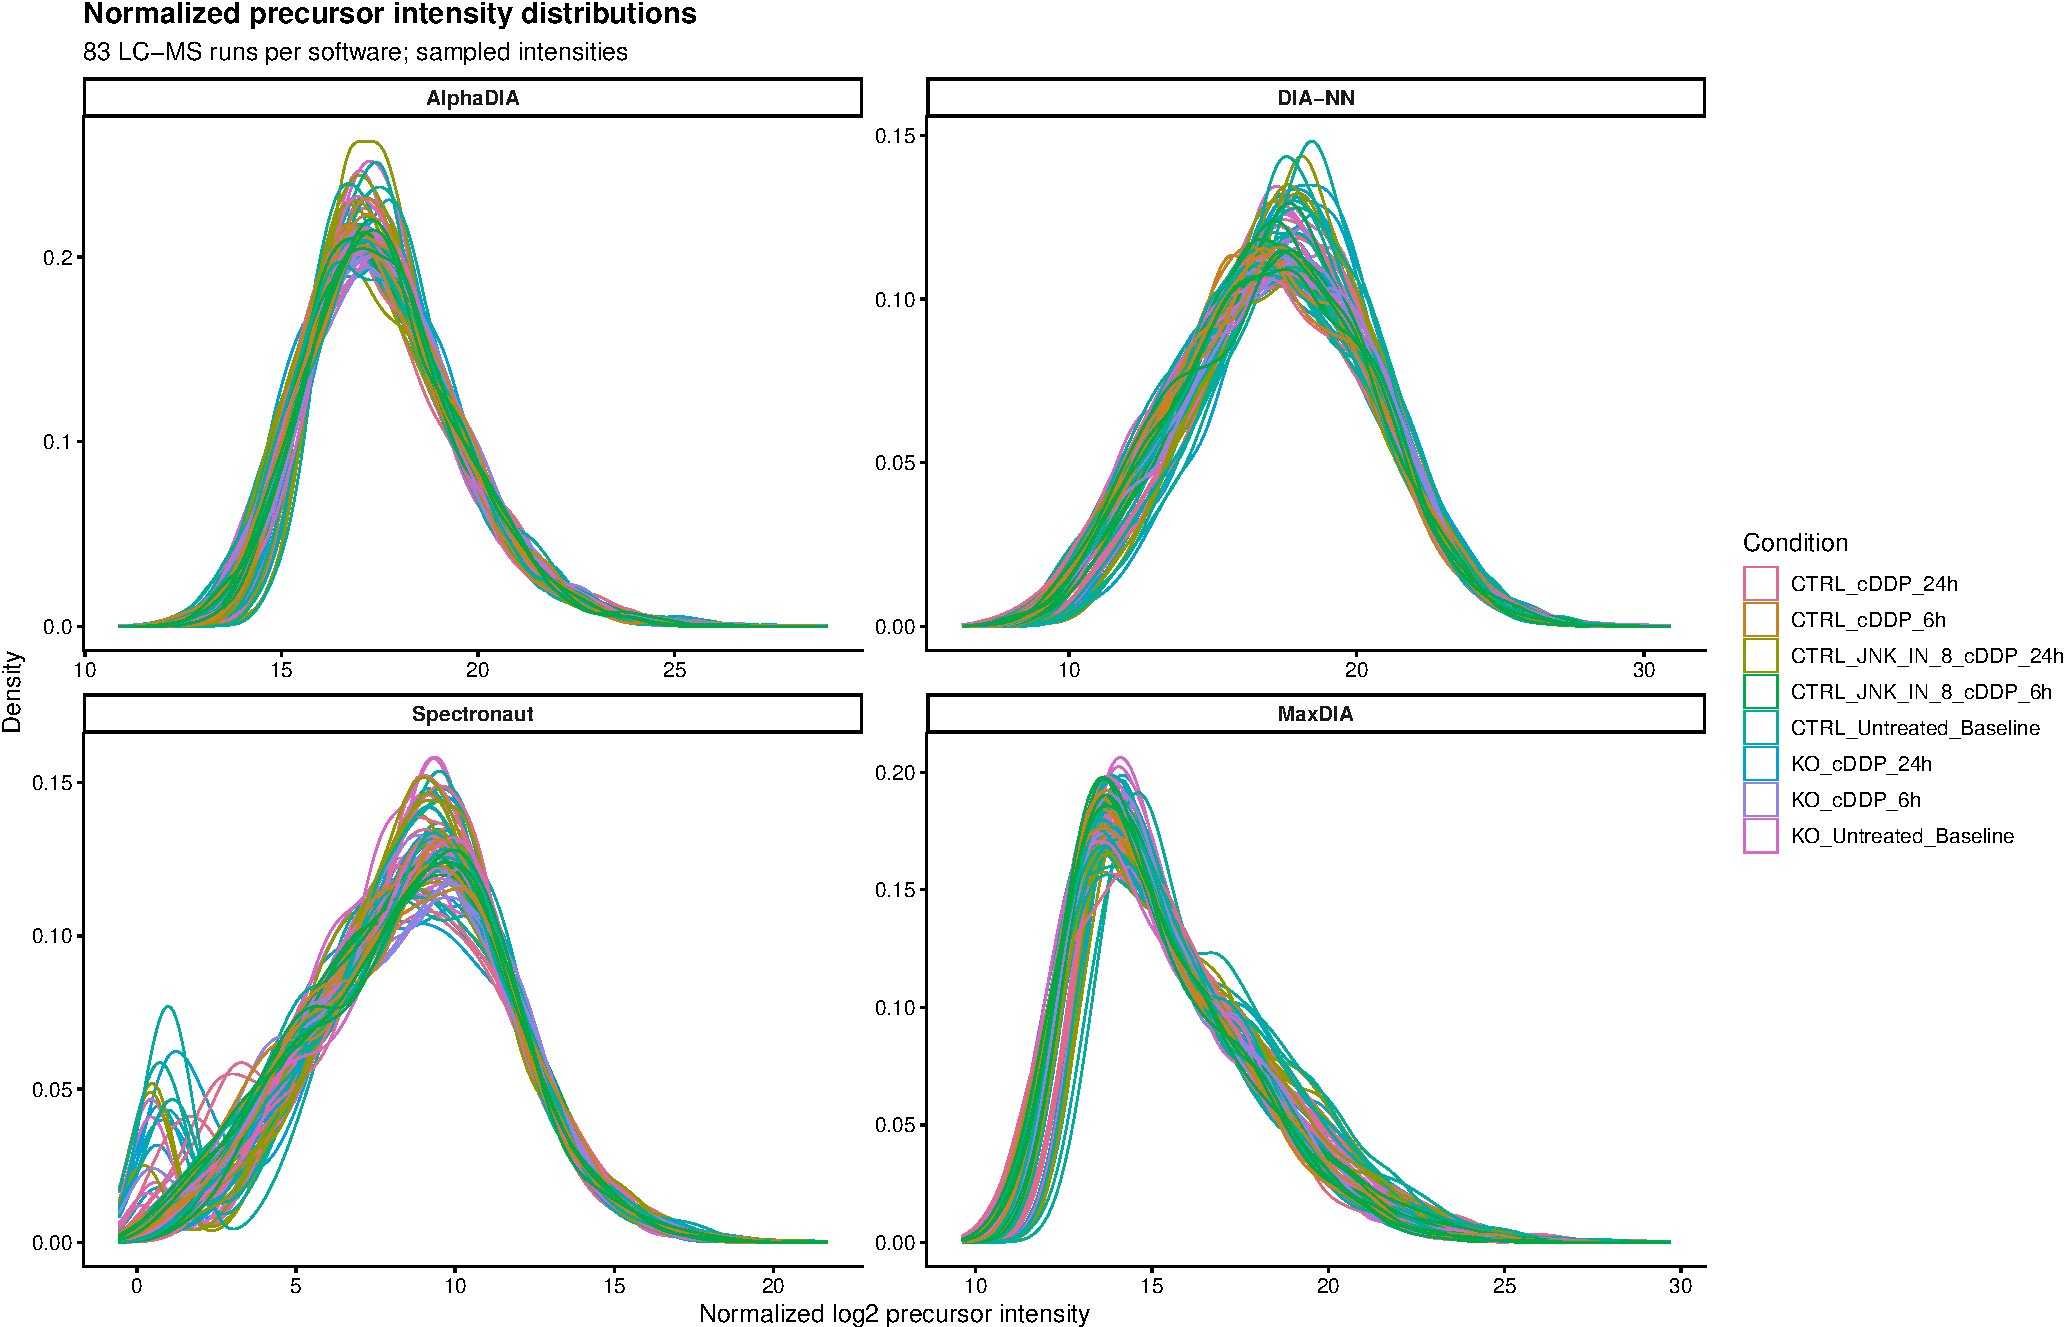
\includegraphics[width=1\linewidth]{DIA_CapstoneProject2026_files/figure-latex/qc_precursor_density-1} \end{center}

\begin{center}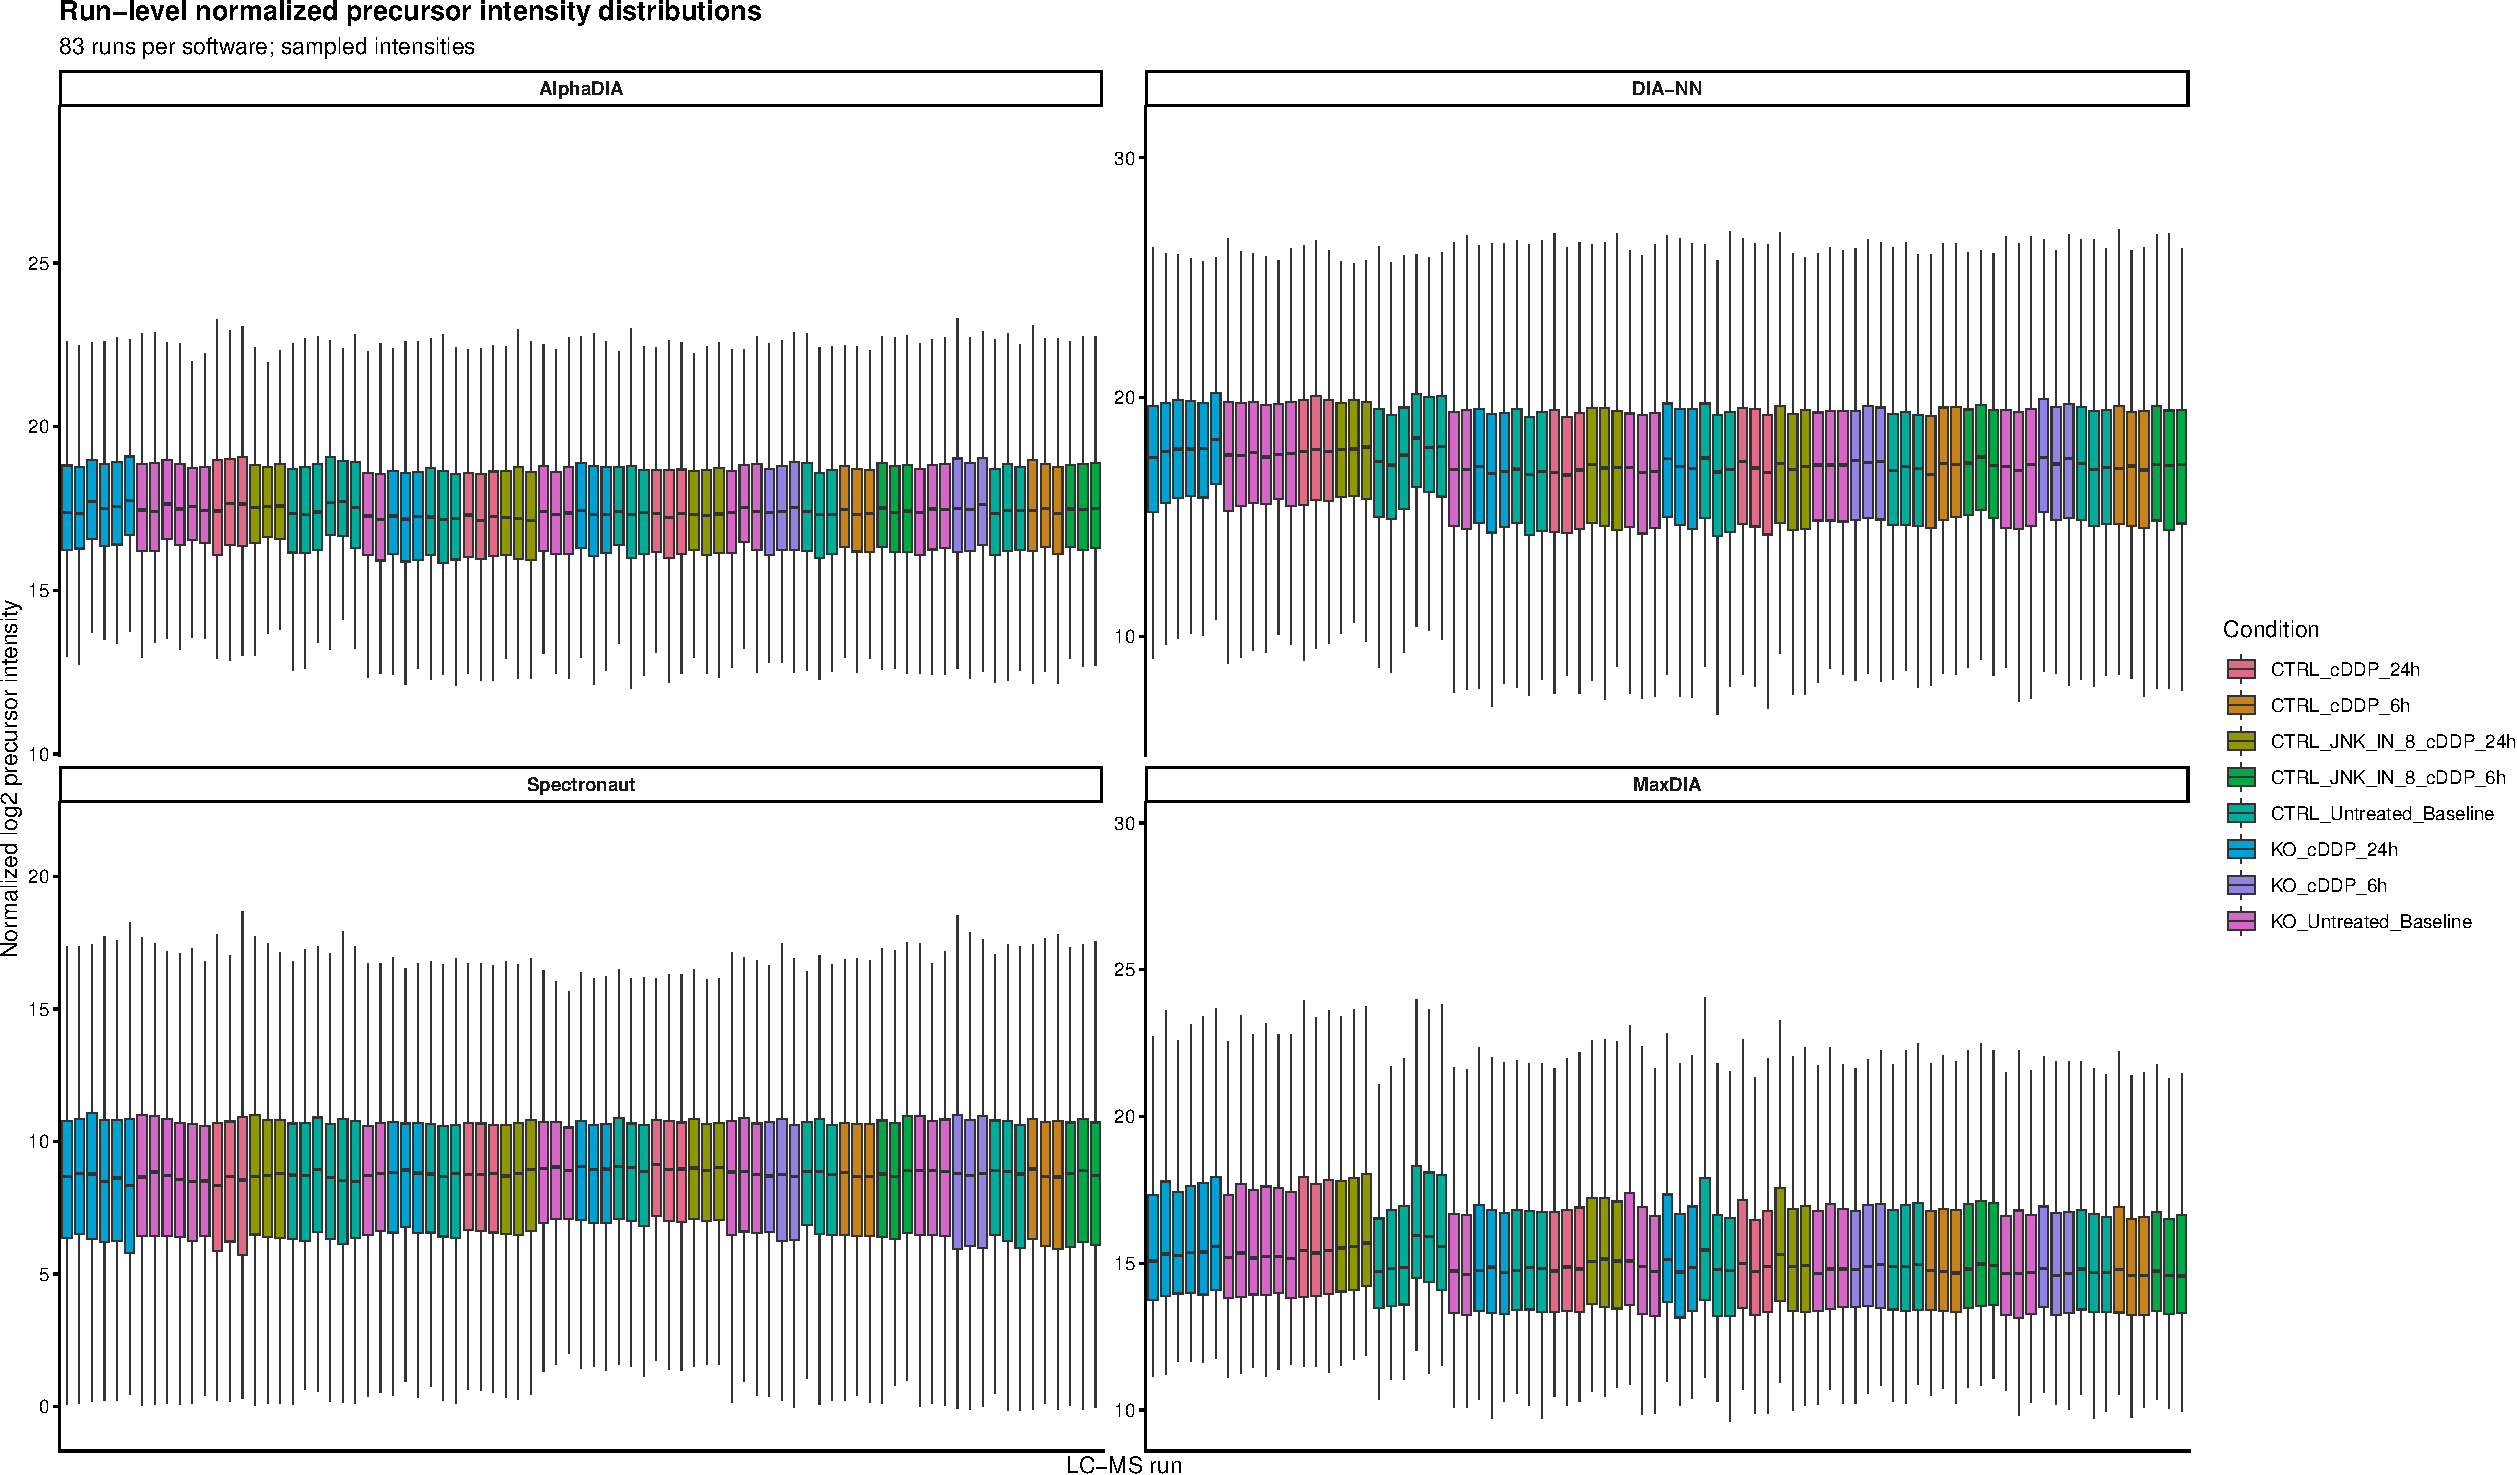
\includegraphics[width=1\linewidth]{DIA_CapstoneProject2026_files/figure-latex/qc_precursor_boxplots-1} \end{center}

\begin{center}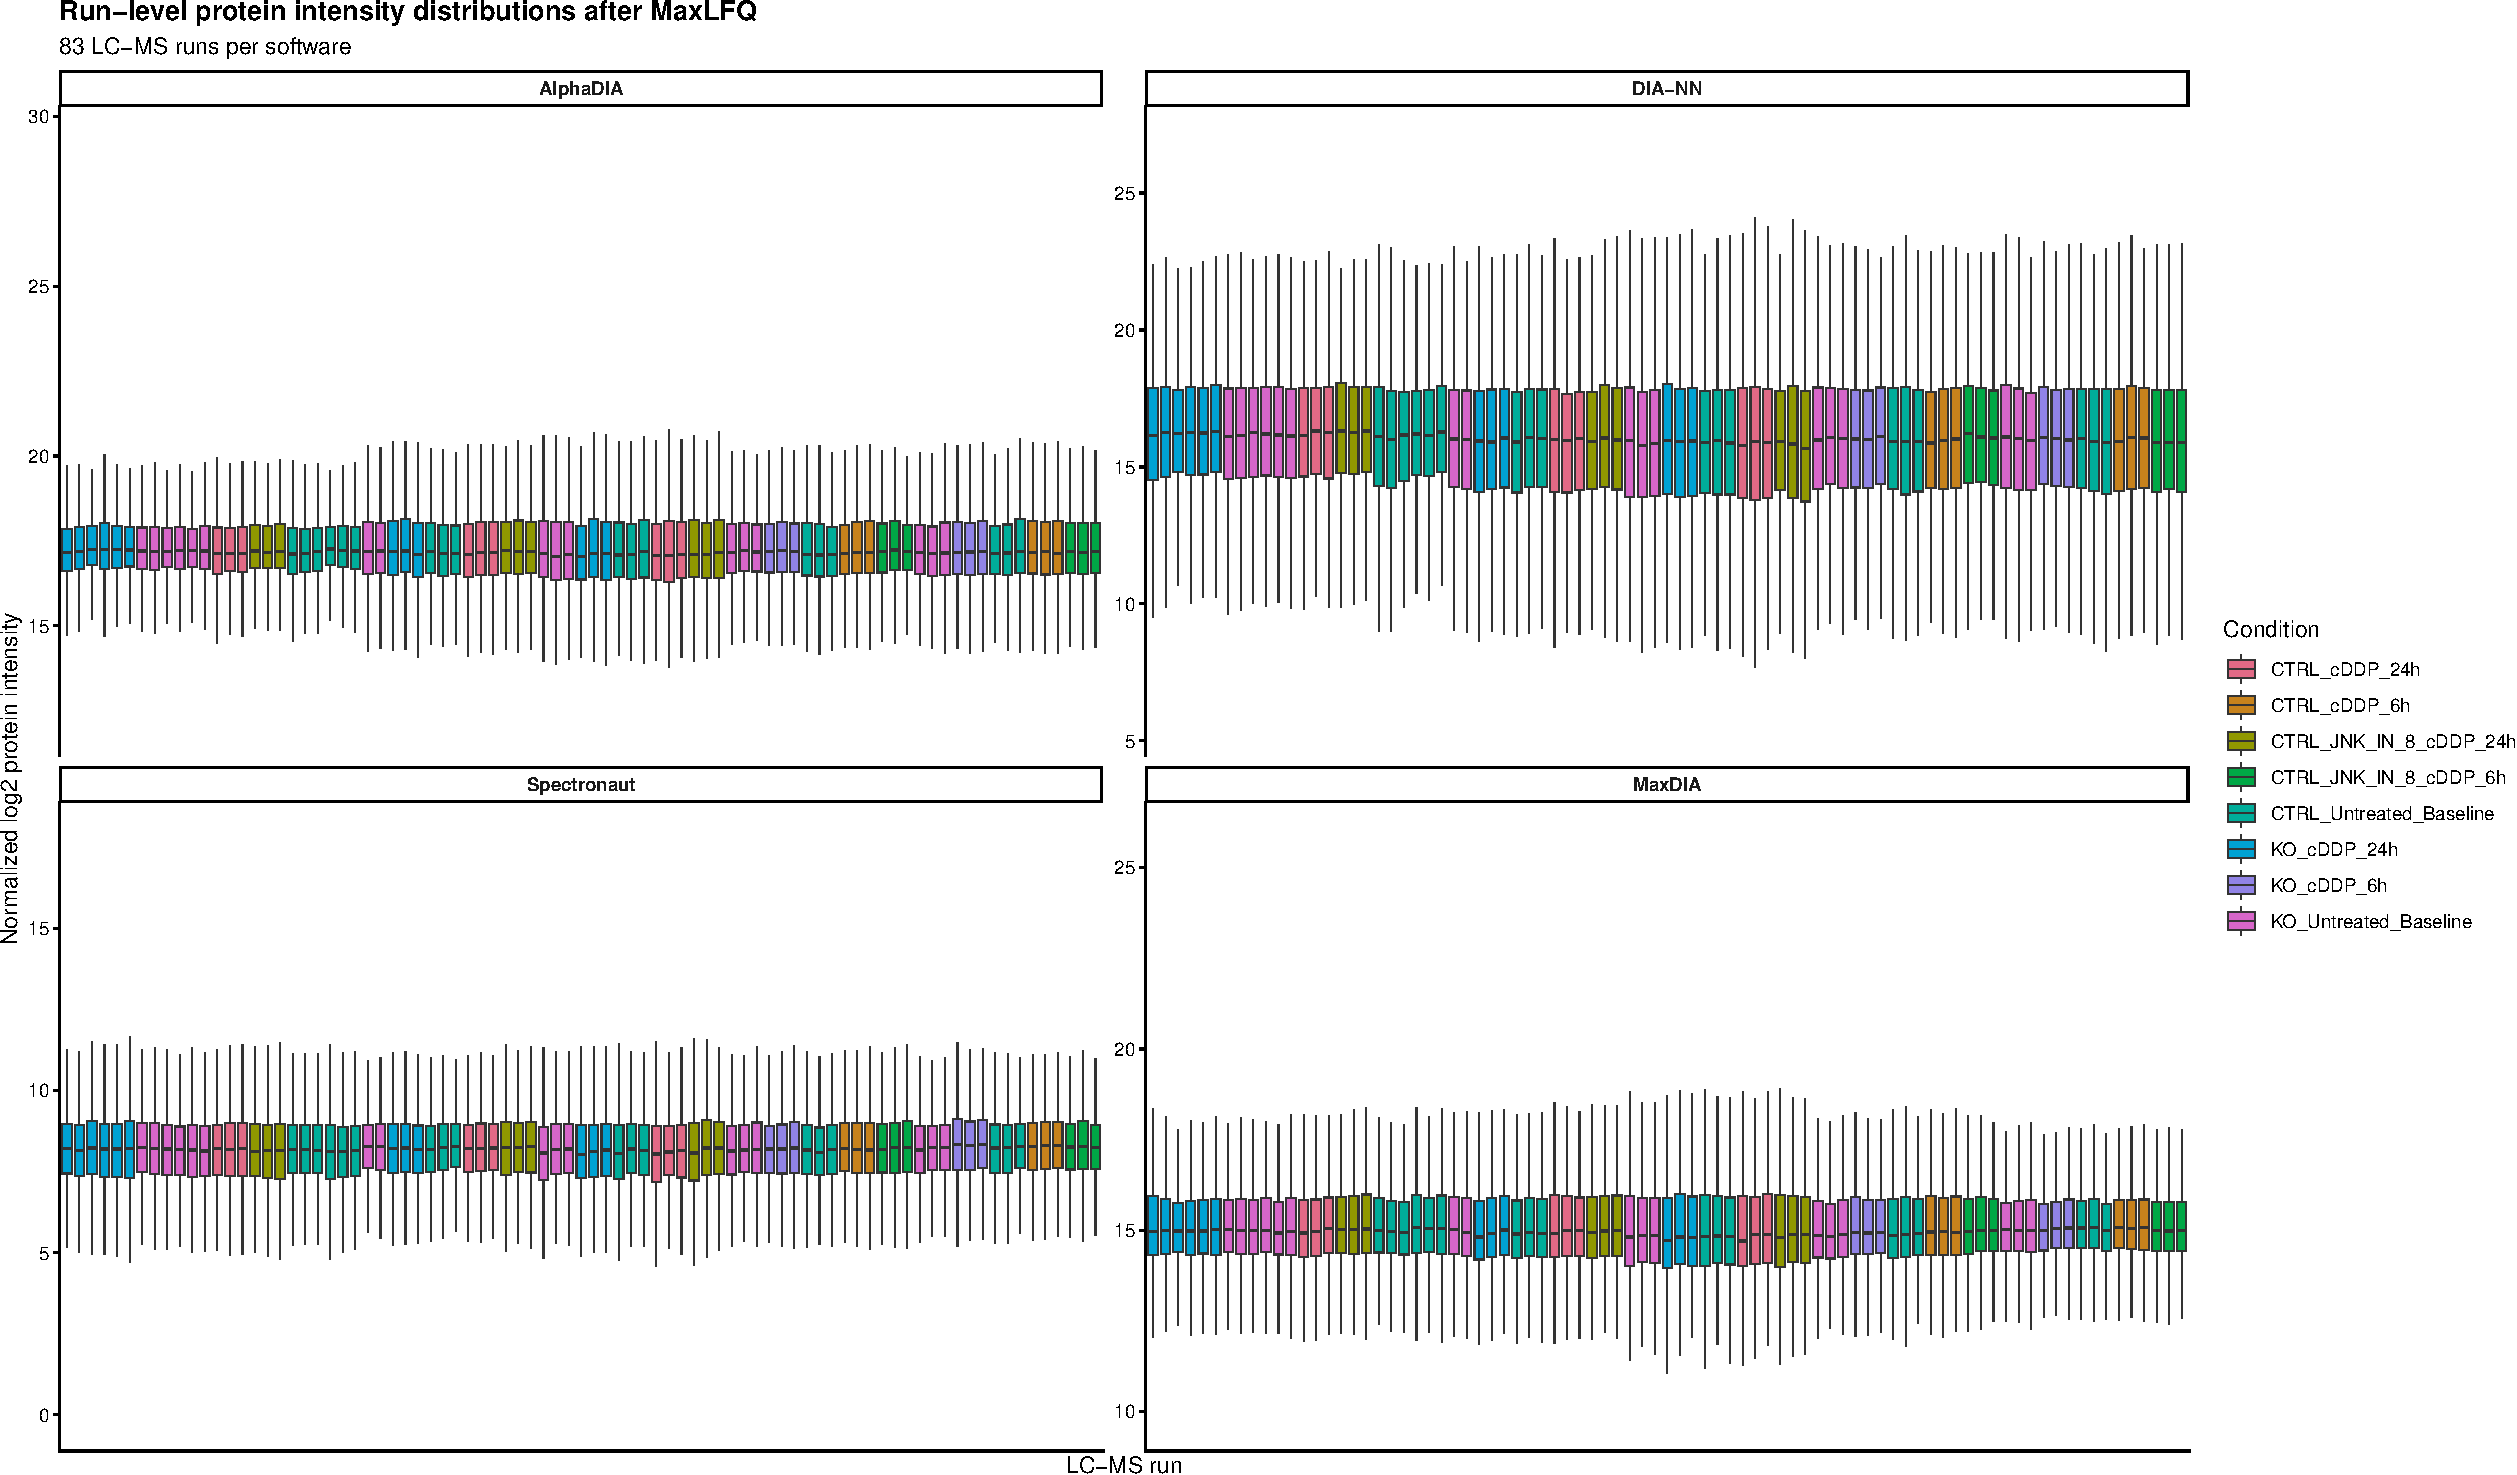
\includegraphics[width=1\linewidth]{DIA_CapstoneProject2026_files/figure-latex/qc_protein_boxplots-1} \end{center}

Overall, the QC results look good and support proceeding to further data
exploration. - Precursor density plots: AlphaDIA and DIA-NN show good
overlap across the 83 runs. MaxDIA has slightly greater variation in
distribution shape, while Spectronaut retains a low-intensity secondary
peak, consistent with its previously observed reporting behavior. -
Precursor boxplots: Run-level medians and intensity ranges are generally
consistent within each software, with no obvious extreme outliers. There
is no clear condition-specific separation in the marginal distributions.
- Protein boxplots: MaxLFQ aggregation produces well-aligned protein
intensity distributions across runs. AlphaDIA and Spectronaut show
particularly tight median alignment, while DIA-NN and MaxDIA exhibit
modest variability.

Normalization and protein aggregation appear successful, with no major
remaining run-level distribution anomalies. However, Spectronaut's
low-intensity behavior warrants continued attention.

\subsection{Charge state}\label{charge-state}

\begin{verbatim}
##      Software       Charge_Source Total_Precursors Charge_1_to_4 Missing_Charge
## 1    AlphaDIA    Precursor.Charge           203024        203024              0
## 2      DIA-NN    Precursor.Charge           206959        206959              0
## 3 Spectronaut Precursor.Id suffix           182083        180023              0
## 4      MaxDIA    Precursor.Charge           230167        230167              0
\end{verbatim}

\begin{center}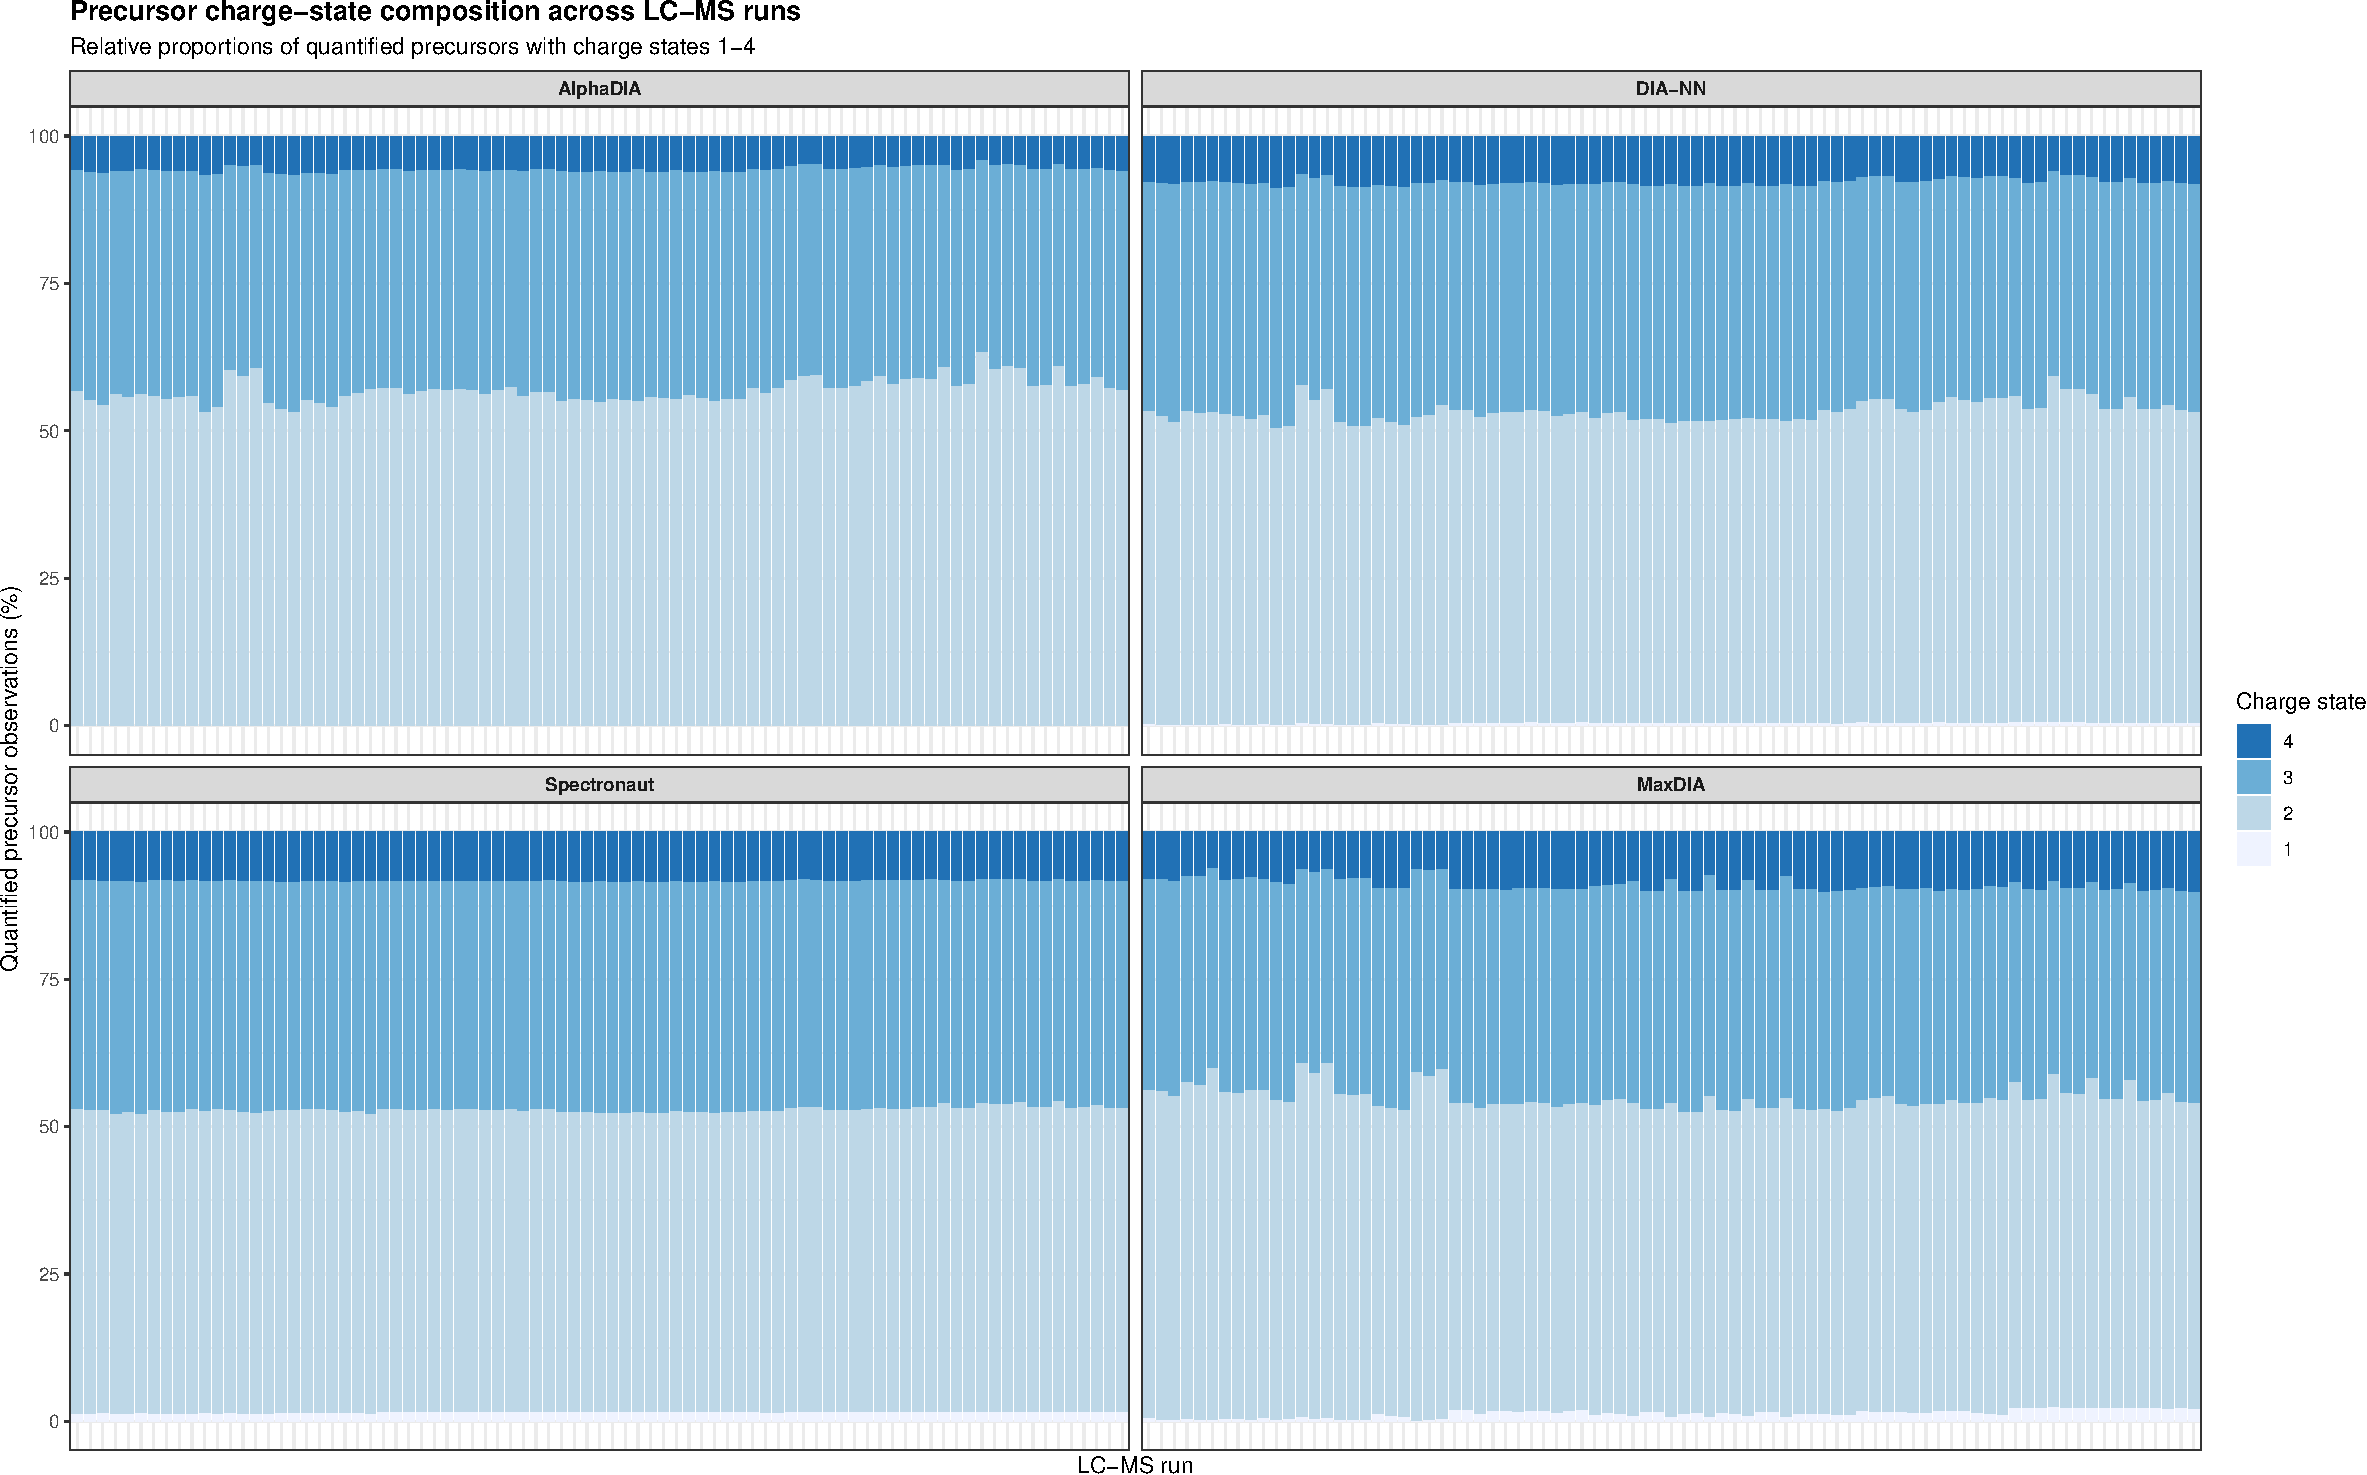
\includegraphics[width=1\linewidth]{DIA_CapstoneProject2026_files/figure-latex/qc_charge_state-1} \end{center}

\begin{verbatim}
## 
##    AlphaDIA      DIA-NN Spectronaut      MaxDIA 
##         249         332         332         332
\end{verbatim}

\begin{center}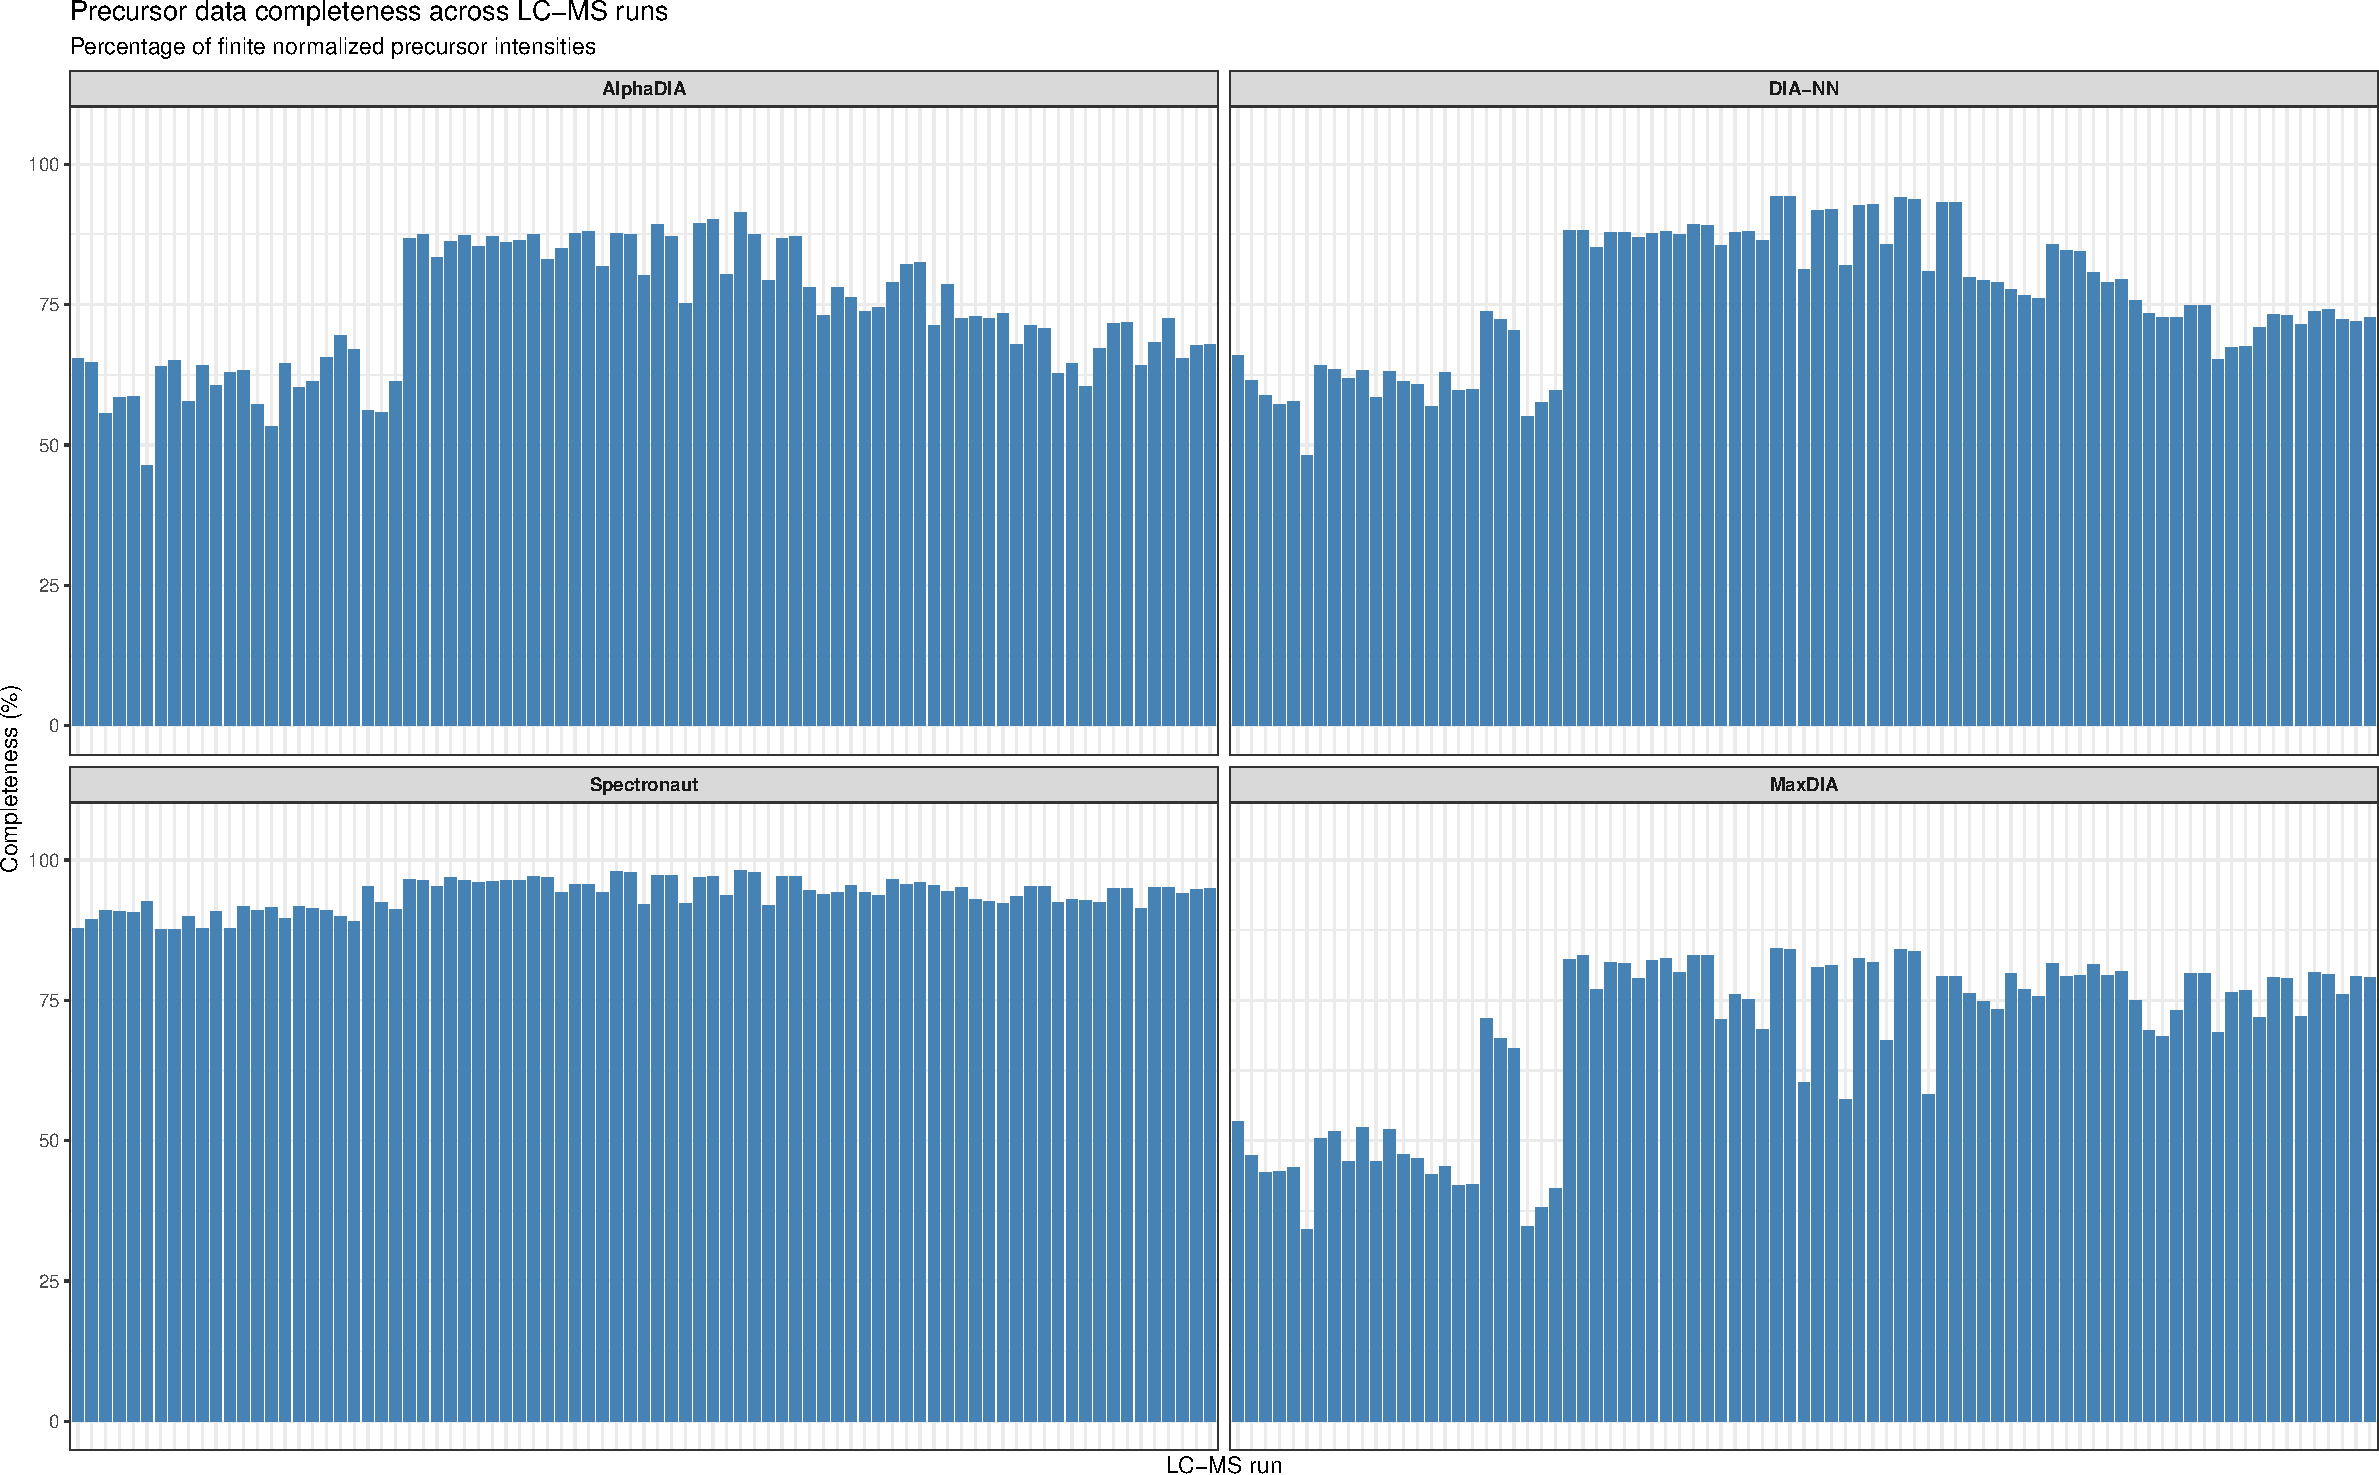
\includegraphics[width=1\linewidth]{DIA_CapstoneProject2026_files/figure-latex/qc_precursor_completeness-1} \end{center}

\begin{verbatim}
##      Software Total_Precursors Runs Min_Run_Completeness
## 1    AlphaDIA           203024   83             46.37481
## 2      DIA-NN           206959   83             48.12789
## 3 Spectronaut           182083   83             87.55128
## 4      MaxDIA           230167   83             34.25469
##   Median_Run_Completeness Max_Run_Completeness Complete_Precursors
## 1                72.53674             91.37787               39666
## 2                75.70630             94.27326               45613
## 3                94.24383             98.04320               75295
## 4                75.95963             84.27185               22251
##   Complete_Precursors_Percent
## 1                   19.537592
## 2                   22.039631
## 3                   41.352021
## 4                    9.667329
\end{verbatim}

The charge-state distributions are generally stable across the 83 LC-MS
runs in all four software pipelines, with predominantly doubly and
triply charged precursors and no obvious major charge-state bias.
However, precursor completeness differs substantially between pipelines.
Spectronaut shows the highest median run-level completeness (94.2\%) and
proportion of precursors quantified across all 83 runs (41.4\%),
although this should be interpreted cautiously given its previously
observed intensity-floor behavior. AlphaDIA and DIA-NN show comparable
median completeness (72.5\% and 75.7\%) and complete precursor
proportions (19.5\% and 22.0\%), whereas MaxDIA exhibits greater
variability, including the lowest minimum run completeness (34.3\%) and
lowest proportion of complete precursors (9.7\%). Overall, charge-state
composition appears consistent, but differences in precursor
missingness---particularly in MaxDIA---should be considered during
downstream statistical modeling.

\subsection{Identifications per
sample}\label{identifications-per-sample}

\begin{center}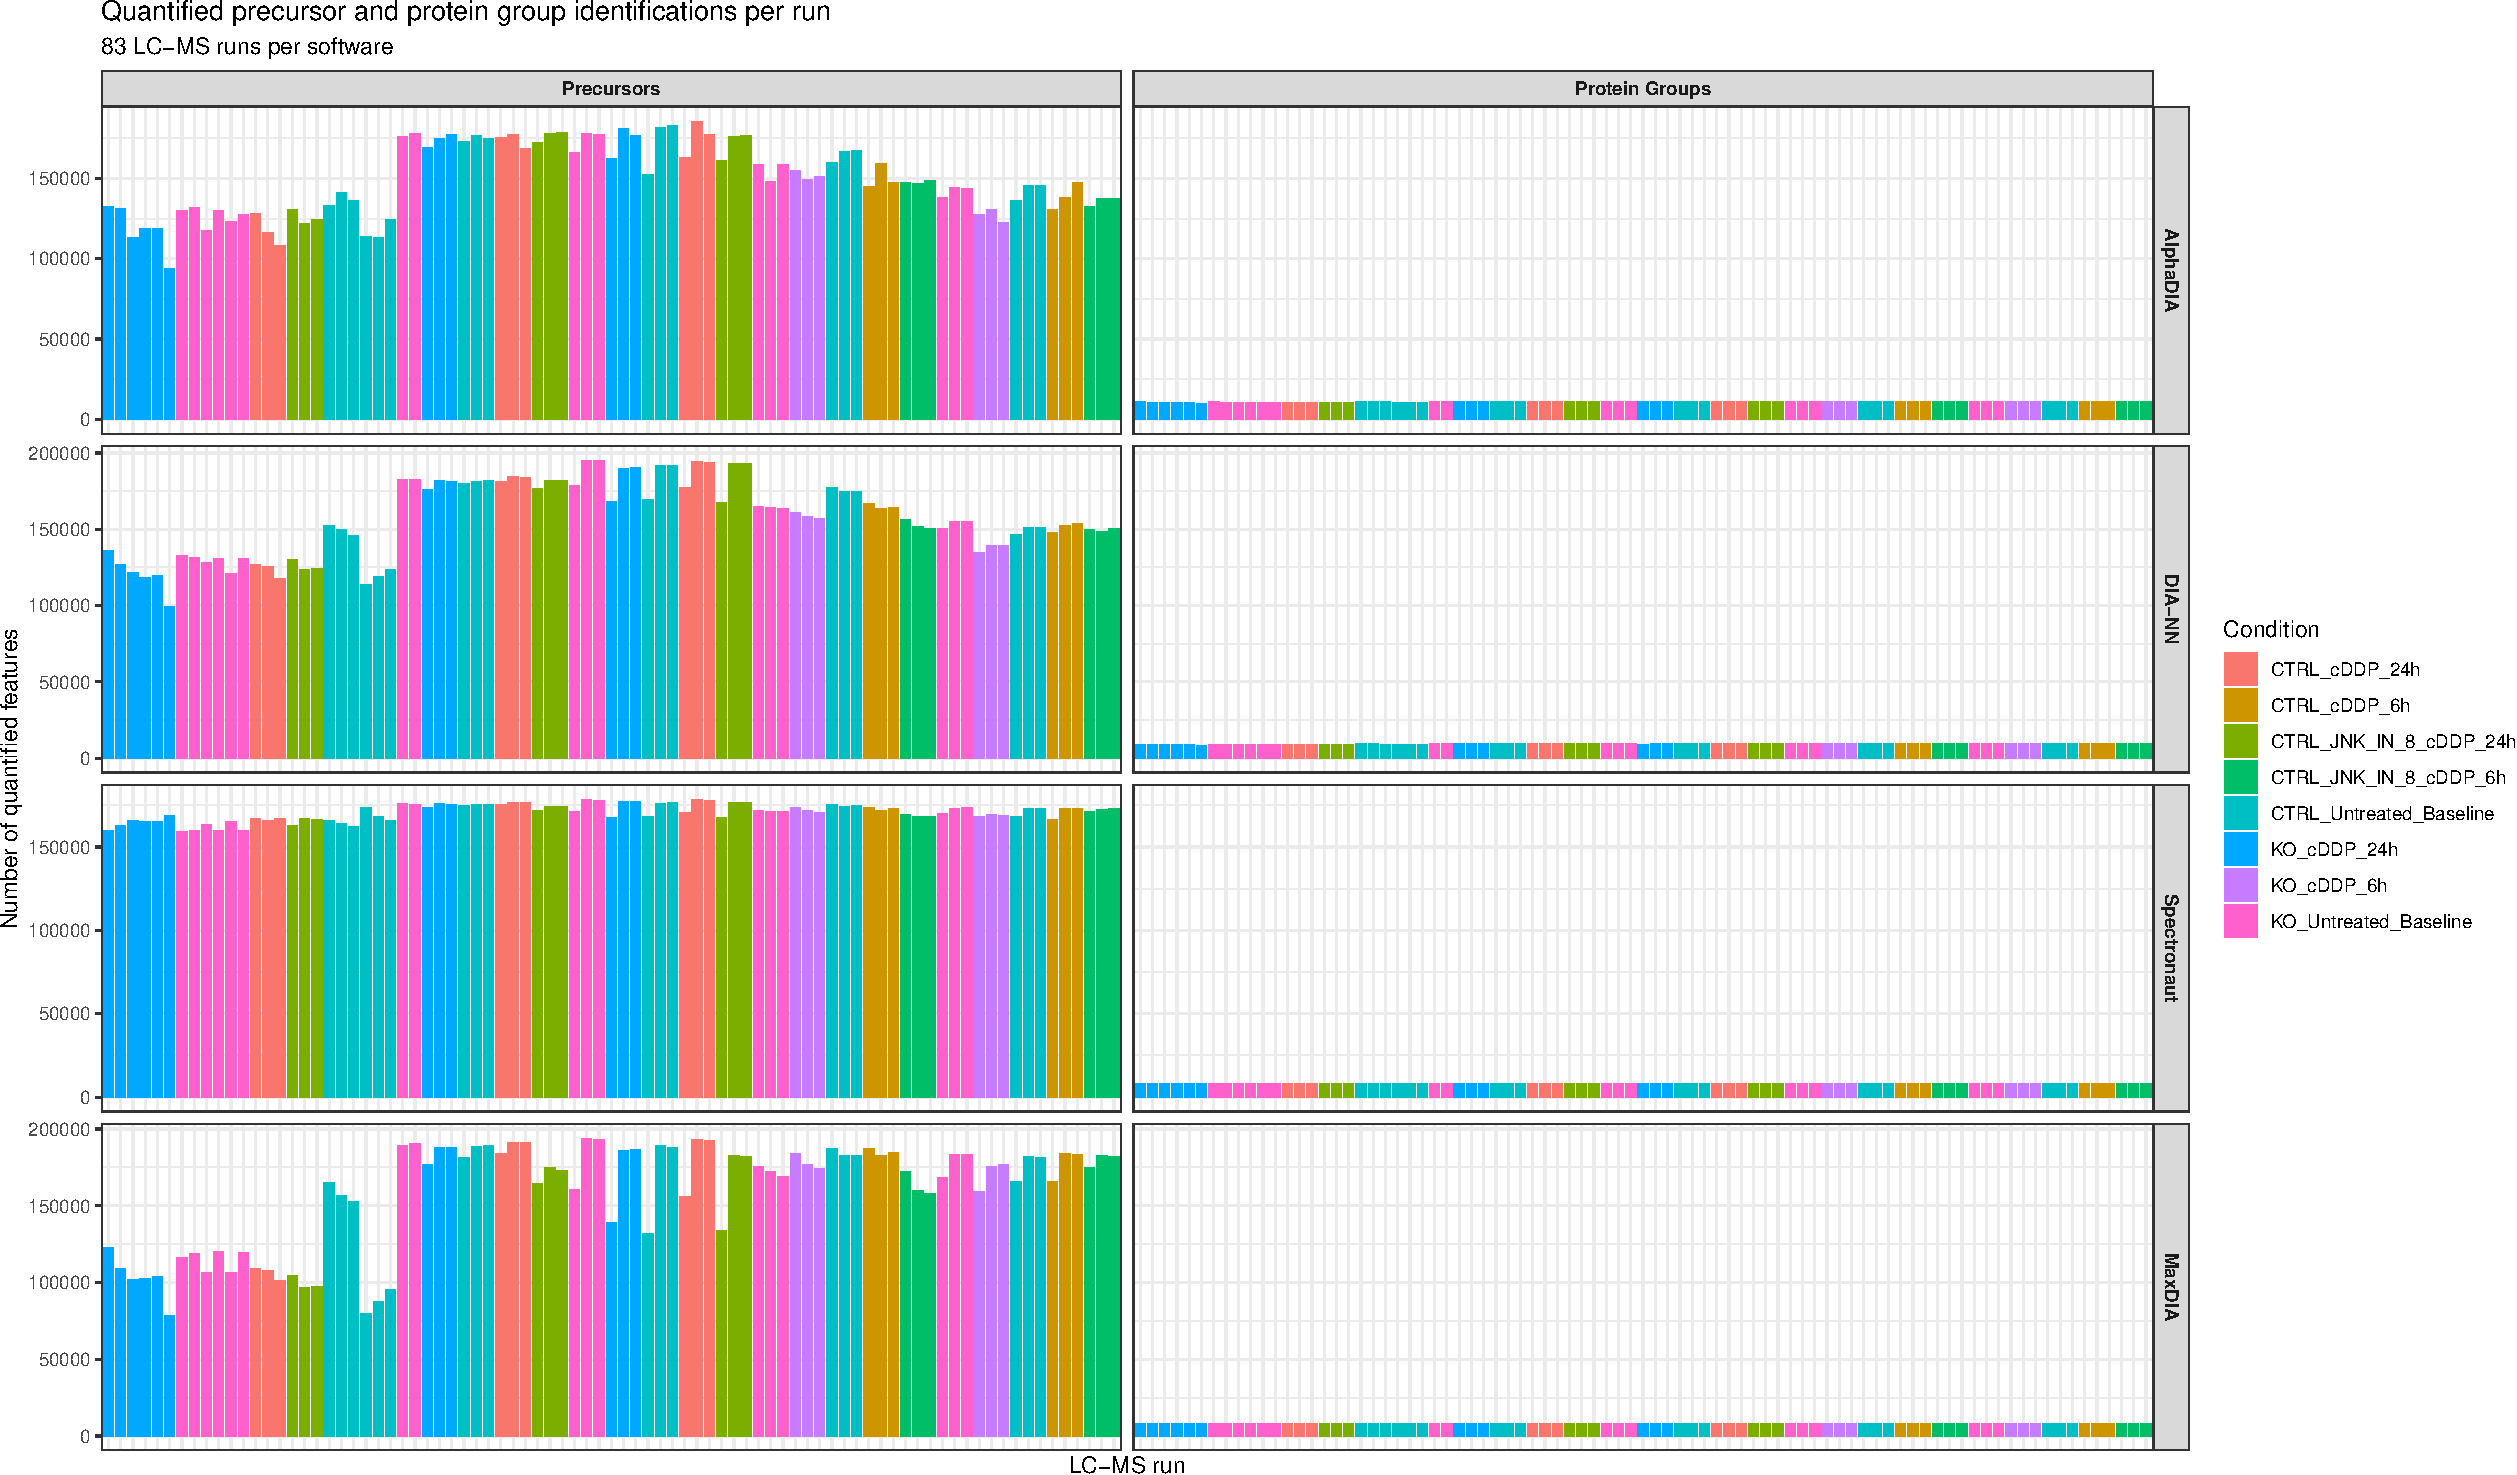
\includegraphics[width=1\linewidth]{DIA_CapstoneProject2026_files/figure-latex/qc_identifications_per_run-1} \end{center}

The number of quantified precursors varies across runs and software
pipelines, with AlphaDIA and DIA-NN showing relatively similar coverage
patterns, Spectronaut exhibiting more consistent precursor counts, and
MaxDIA displaying greater run-to-run variability. Protein group counts
appear comparatively stable within each pipeline. These results suggest
differences in precursor detection efficiency and coverage between
software tools, without indicating a clear condition-specific
identification bias.

\begin{center}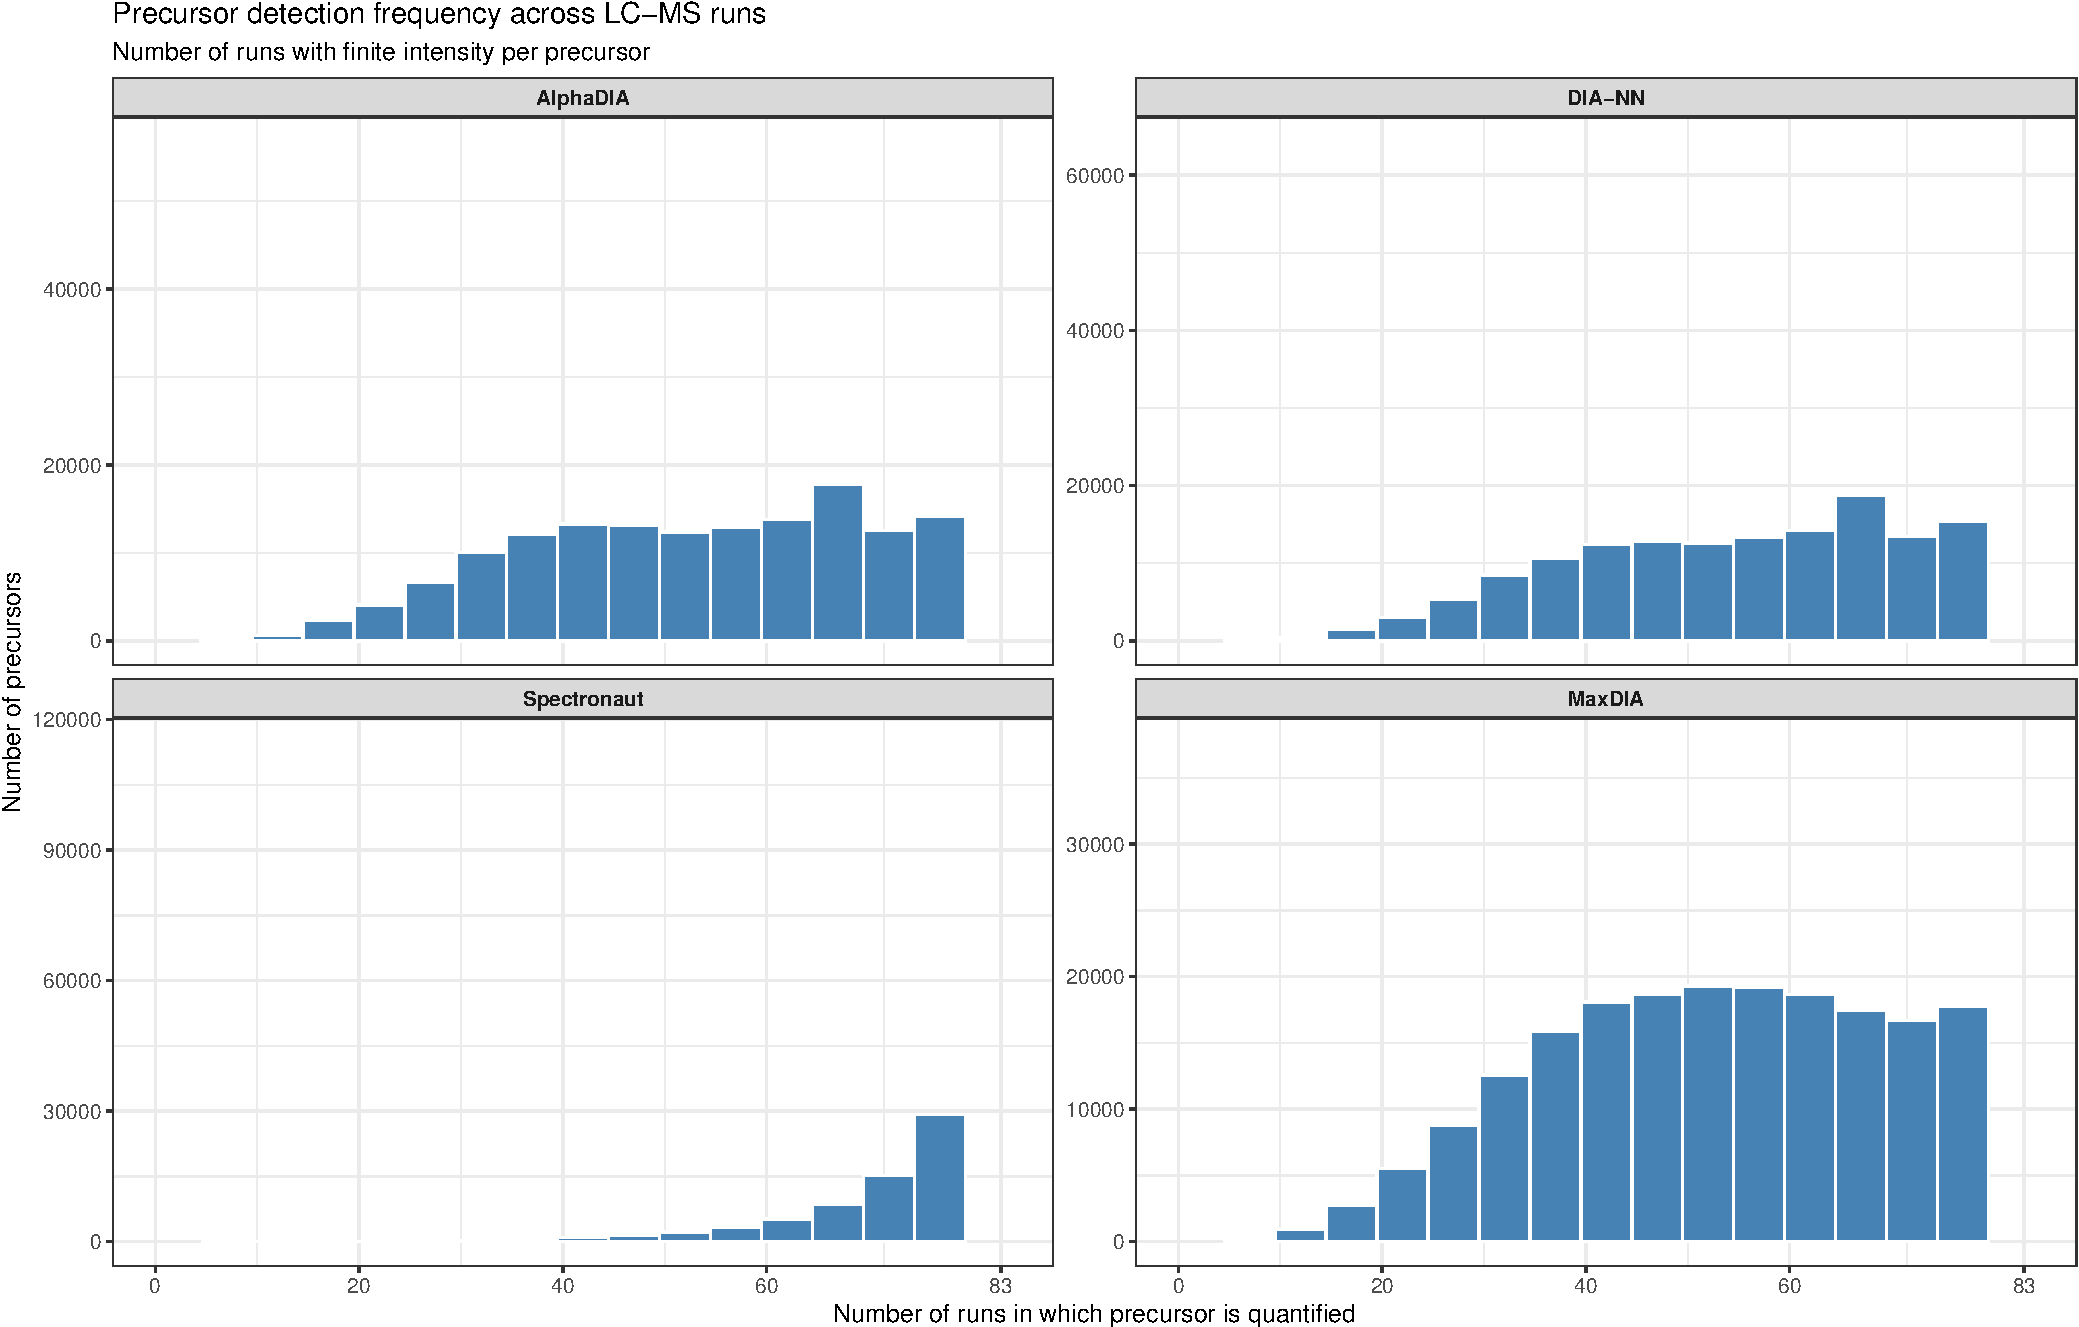
\includegraphics[width=1\linewidth]{DIA_CapstoneProject2026_files/figure-latex/qc_precursor_detection_frequency-1} \end{center}

Precursor detection frequency differs substantially between software
packages. Spectronaut shows a strong concentration of precursors
quantified in nearly all 83 runs, indicating high data completeness.
AlphaDIA and DIA-NN exhibit broader detection-frequency distributions,
while MaxDIA shows the greatest proportion of precursors quantified in
intermediate numbers of runs. These findings highlight
software-dependent missingness patterns, with Spectronaut providing the
most complete precursor matrix, although its previously observed
intensity-floor behavior warrants caution.

\begin{center}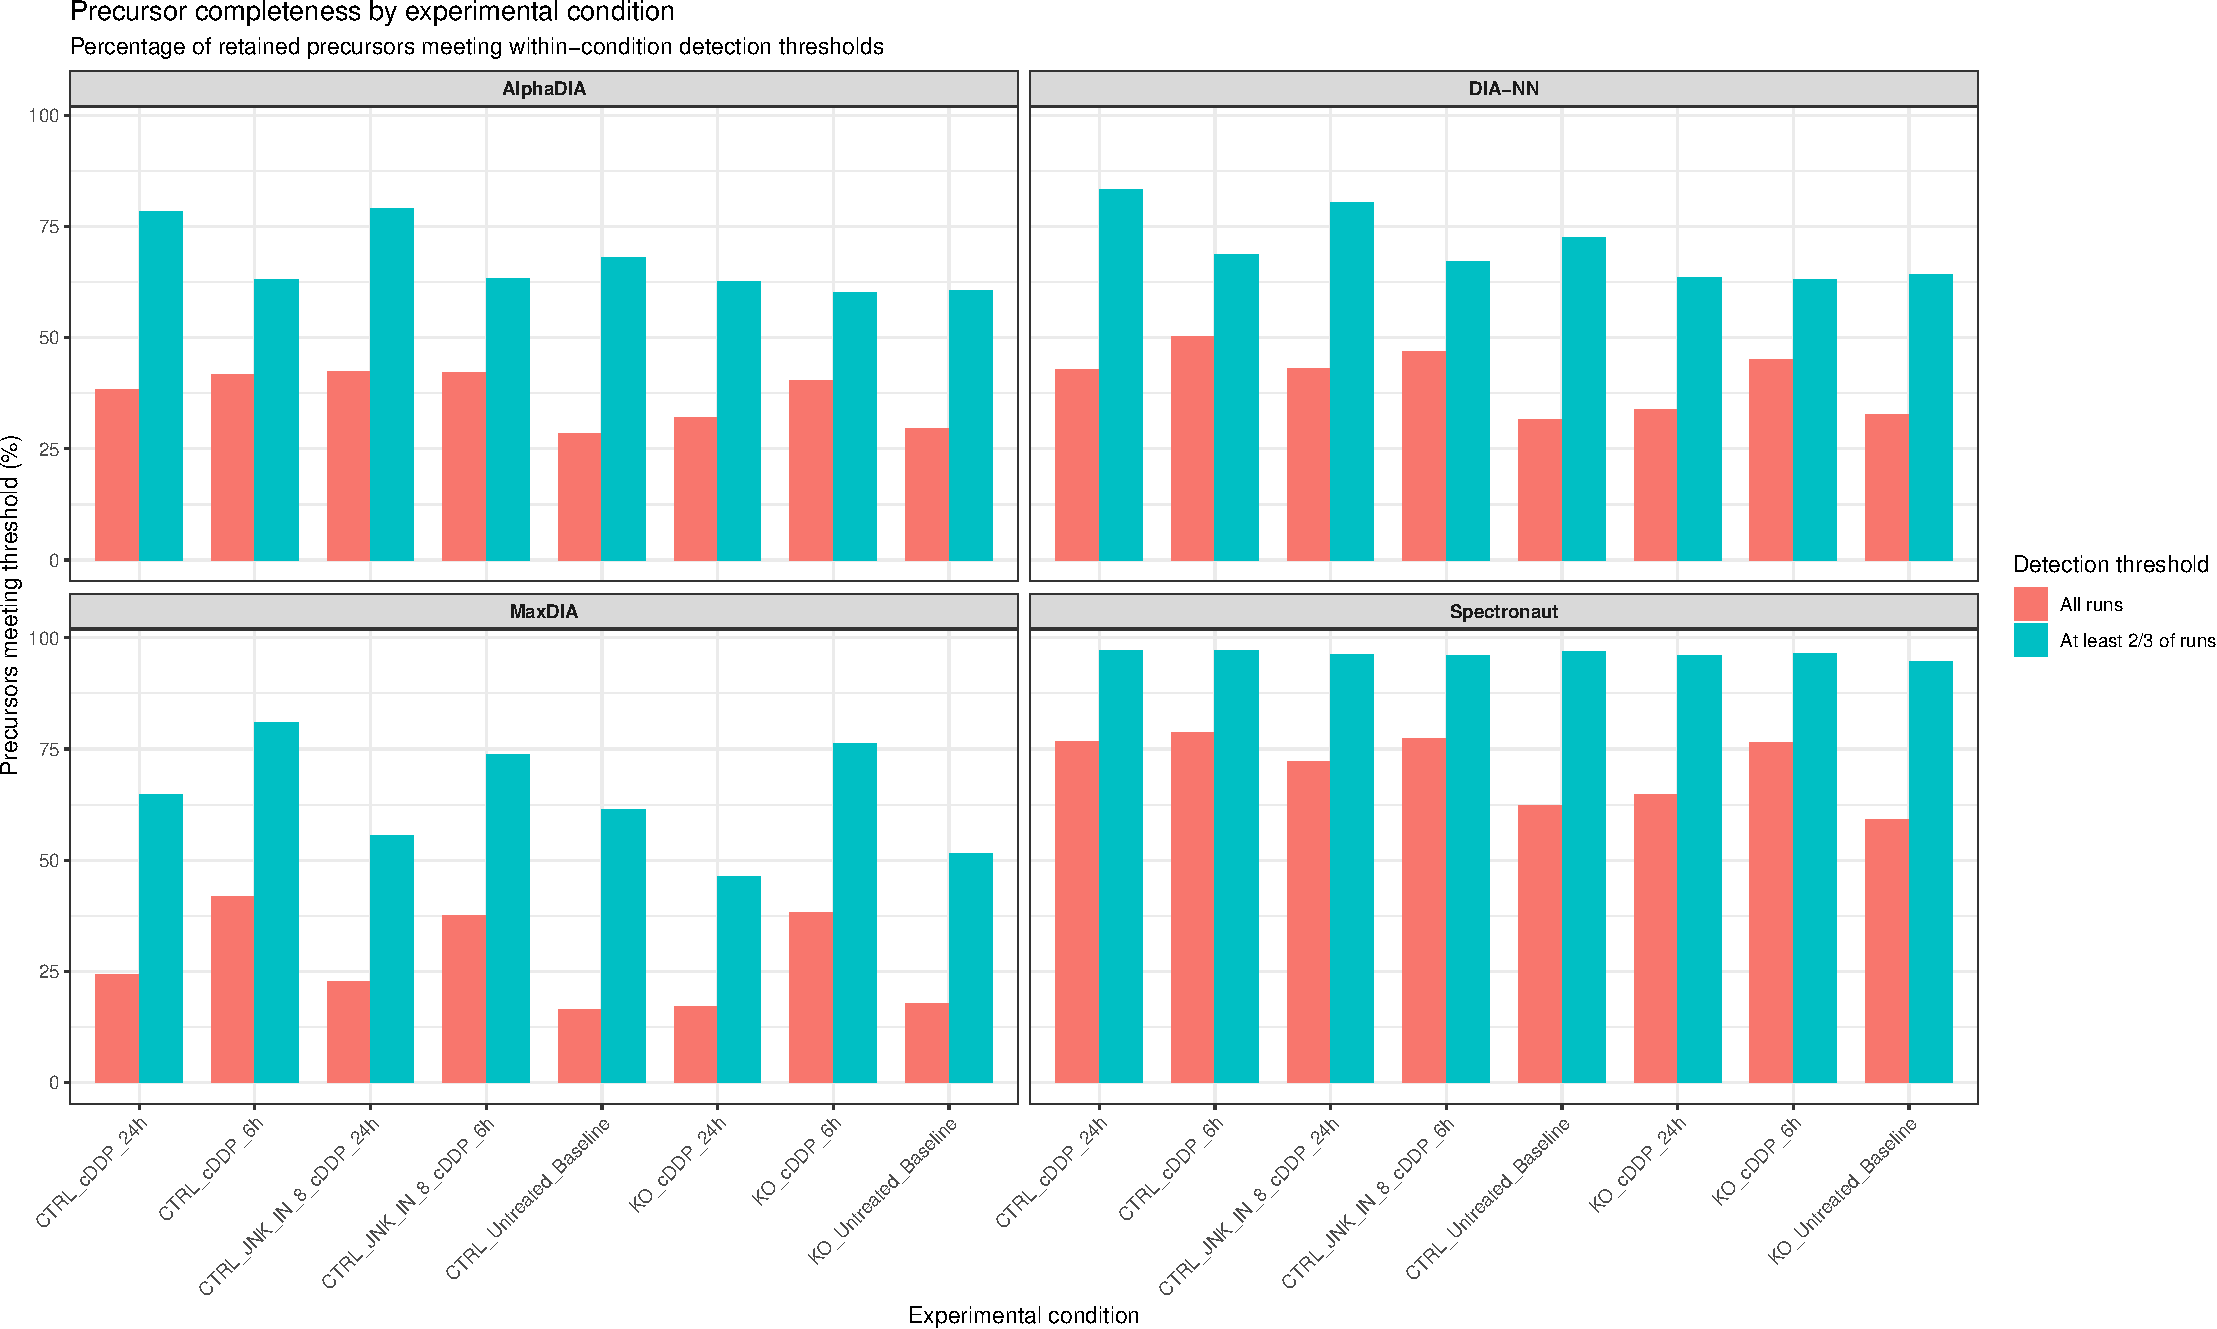
\includegraphics[width=1\linewidth]{DIA_CapstoneProject2026_files/figure-latex/qc_completeness_by_condition-1} \end{center}

\begin{verbatim}
##       Software               Condition Runs Complete_Percent Two_Thirds_Percent
## 1     AlphaDIA           CTRL_cDDP_24h    9         38.44718           78.34640
## 2     AlphaDIA            CTRL_cDDP_6h    6         41.67635           63.16889
## 3     AlphaDIA  CTRL_JNK_IN_8_cDDP_24h    9         42.30534           79.01726
## 4     AlphaDIA   CTRL_JNK_IN_8_cDDP_6h    6         42.28219           63.36098
## 5     AlphaDIA CTRL_Untreated_Baseline   18         28.39664           68.07816
## 6     AlphaDIA             KO_cDDP_24h   12         31.96716           62.59309
## 7     AlphaDIA              KO_cDDP_6h    6         40.31346           60.08551
## 8     AlphaDIA   KO_Untreated_Baseline   17         29.66349           60.65539
## 9       DIA-NN           CTRL_cDDP_24h    9         42.81669           83.31892
## 10      DIA-NN            CTRL_cDDP_6h    6         50.15969           68.61697
## 11      DIA-NN  CTRL_JNK_IN_8_cDDP_24h    9         43.16266           80.49420
## 12      DIA-NN   CTRL_JNK_IN_8_cDDP_6h    6         46.95761           67.16113
## 13      DIA-NN CTRL_Untreated_Baseline   18         31.71643           72.53466
## 14      DIA-NN             KO_cDDP_24h   12         33.87338           63.50871
## 15      DIA-NN              KO_cDDP_6h    6         45.10749           63.04389
## 16      DIA-NN   KO_Untreated_Baseline   17         32.72532           64.13009
## 17 Spectronaut           CTRL_cDDP_24h    9         76.58266           97.13812
## 18 Spectronaut            CTRL_cDDP_6h    6         78.78111           97.12329
## 19 Spectronaut  CTRL_JNK_IN_8_cDDP_24h    9         72.13084           96.30443
## 20 Spectronaut   CTRL_JNK_IN_8_cDDP_6h    6         77.33781           96.07267
## 21 Spectronaut CTRL_Untreated_Baseline   18         62.29906           96.82453
## 22 Spectronaut             KO_cDDP_24h   12         64.68863           95.96887
## 23 Spectronaut              KO_cDDP_6h    6         76.52389           96.41098
## 24 Spectronaut   KO_Untreated_Baseline   17         59.16203           94.60301
## 25      MaxDIA           CTRL_cDDP_24h    9         24.26847           64.77644
## 26      MaxDIA            CTRL_cDDP_6h    6         41.77662           80.88518
## 27      MaxDIA  CTRL_JNK_IN_8_cDDP_24h    9         22.81170           55.57834
## 28      MaxDIA   CTRL_JNK_IN_8_cDDP_6h    6         37.52145           73.81075
## 29      MaxDIA CTRL_Untreated_Baseline   18         16.36464           61.33764
## 30      MaxDIA             KO_cDDP_24h   12         17.00591           46.41804
## 31      MaxDIA              KO_cDDP_6h    6         38.26396           76.22856
## 32      MaxDIA   KO_Untreated_Baseline   17         17.78969           51.61383
\end{verbatim}

Spectronaut consistently demonstrates the highest within-condition
completeness, with approximately 59--79\% of precursors quantified in
every replicate and 95--97\% meeting the two-thirds detection threshold.
AlphaDIA and DIA-NN show intermediate completeness, with 28--42\% and
32--50\% of precursors, respectively, quantified in all runs within a
condition. MaxDIA exhibits the lowest and most variable completeness
(16--42\%), particularly in untreated baseline and 24-hour treatment
groups. Across all pipelines, conditions containing more replicates
generally show lower complete-case percentages, reflecting the greater
difficulty of detecting a precursor in every run. Overall, these results
emphasize the importance of accounting for software-specific missingness
during downstream statistical modeling.

\subsection{Dimensionality reduction
plot}\label{dimensionality-reduction-plot}

\begin{verbatim}
##      Software Proteins_Used Runs
## 1    AlphaDIA          8828   83
## 2      DIA-NN          7557   83
## 3 Spectronaut          7581   83
## 4      MaxDIA          7515   83
\end{verbatim}

\begin{center}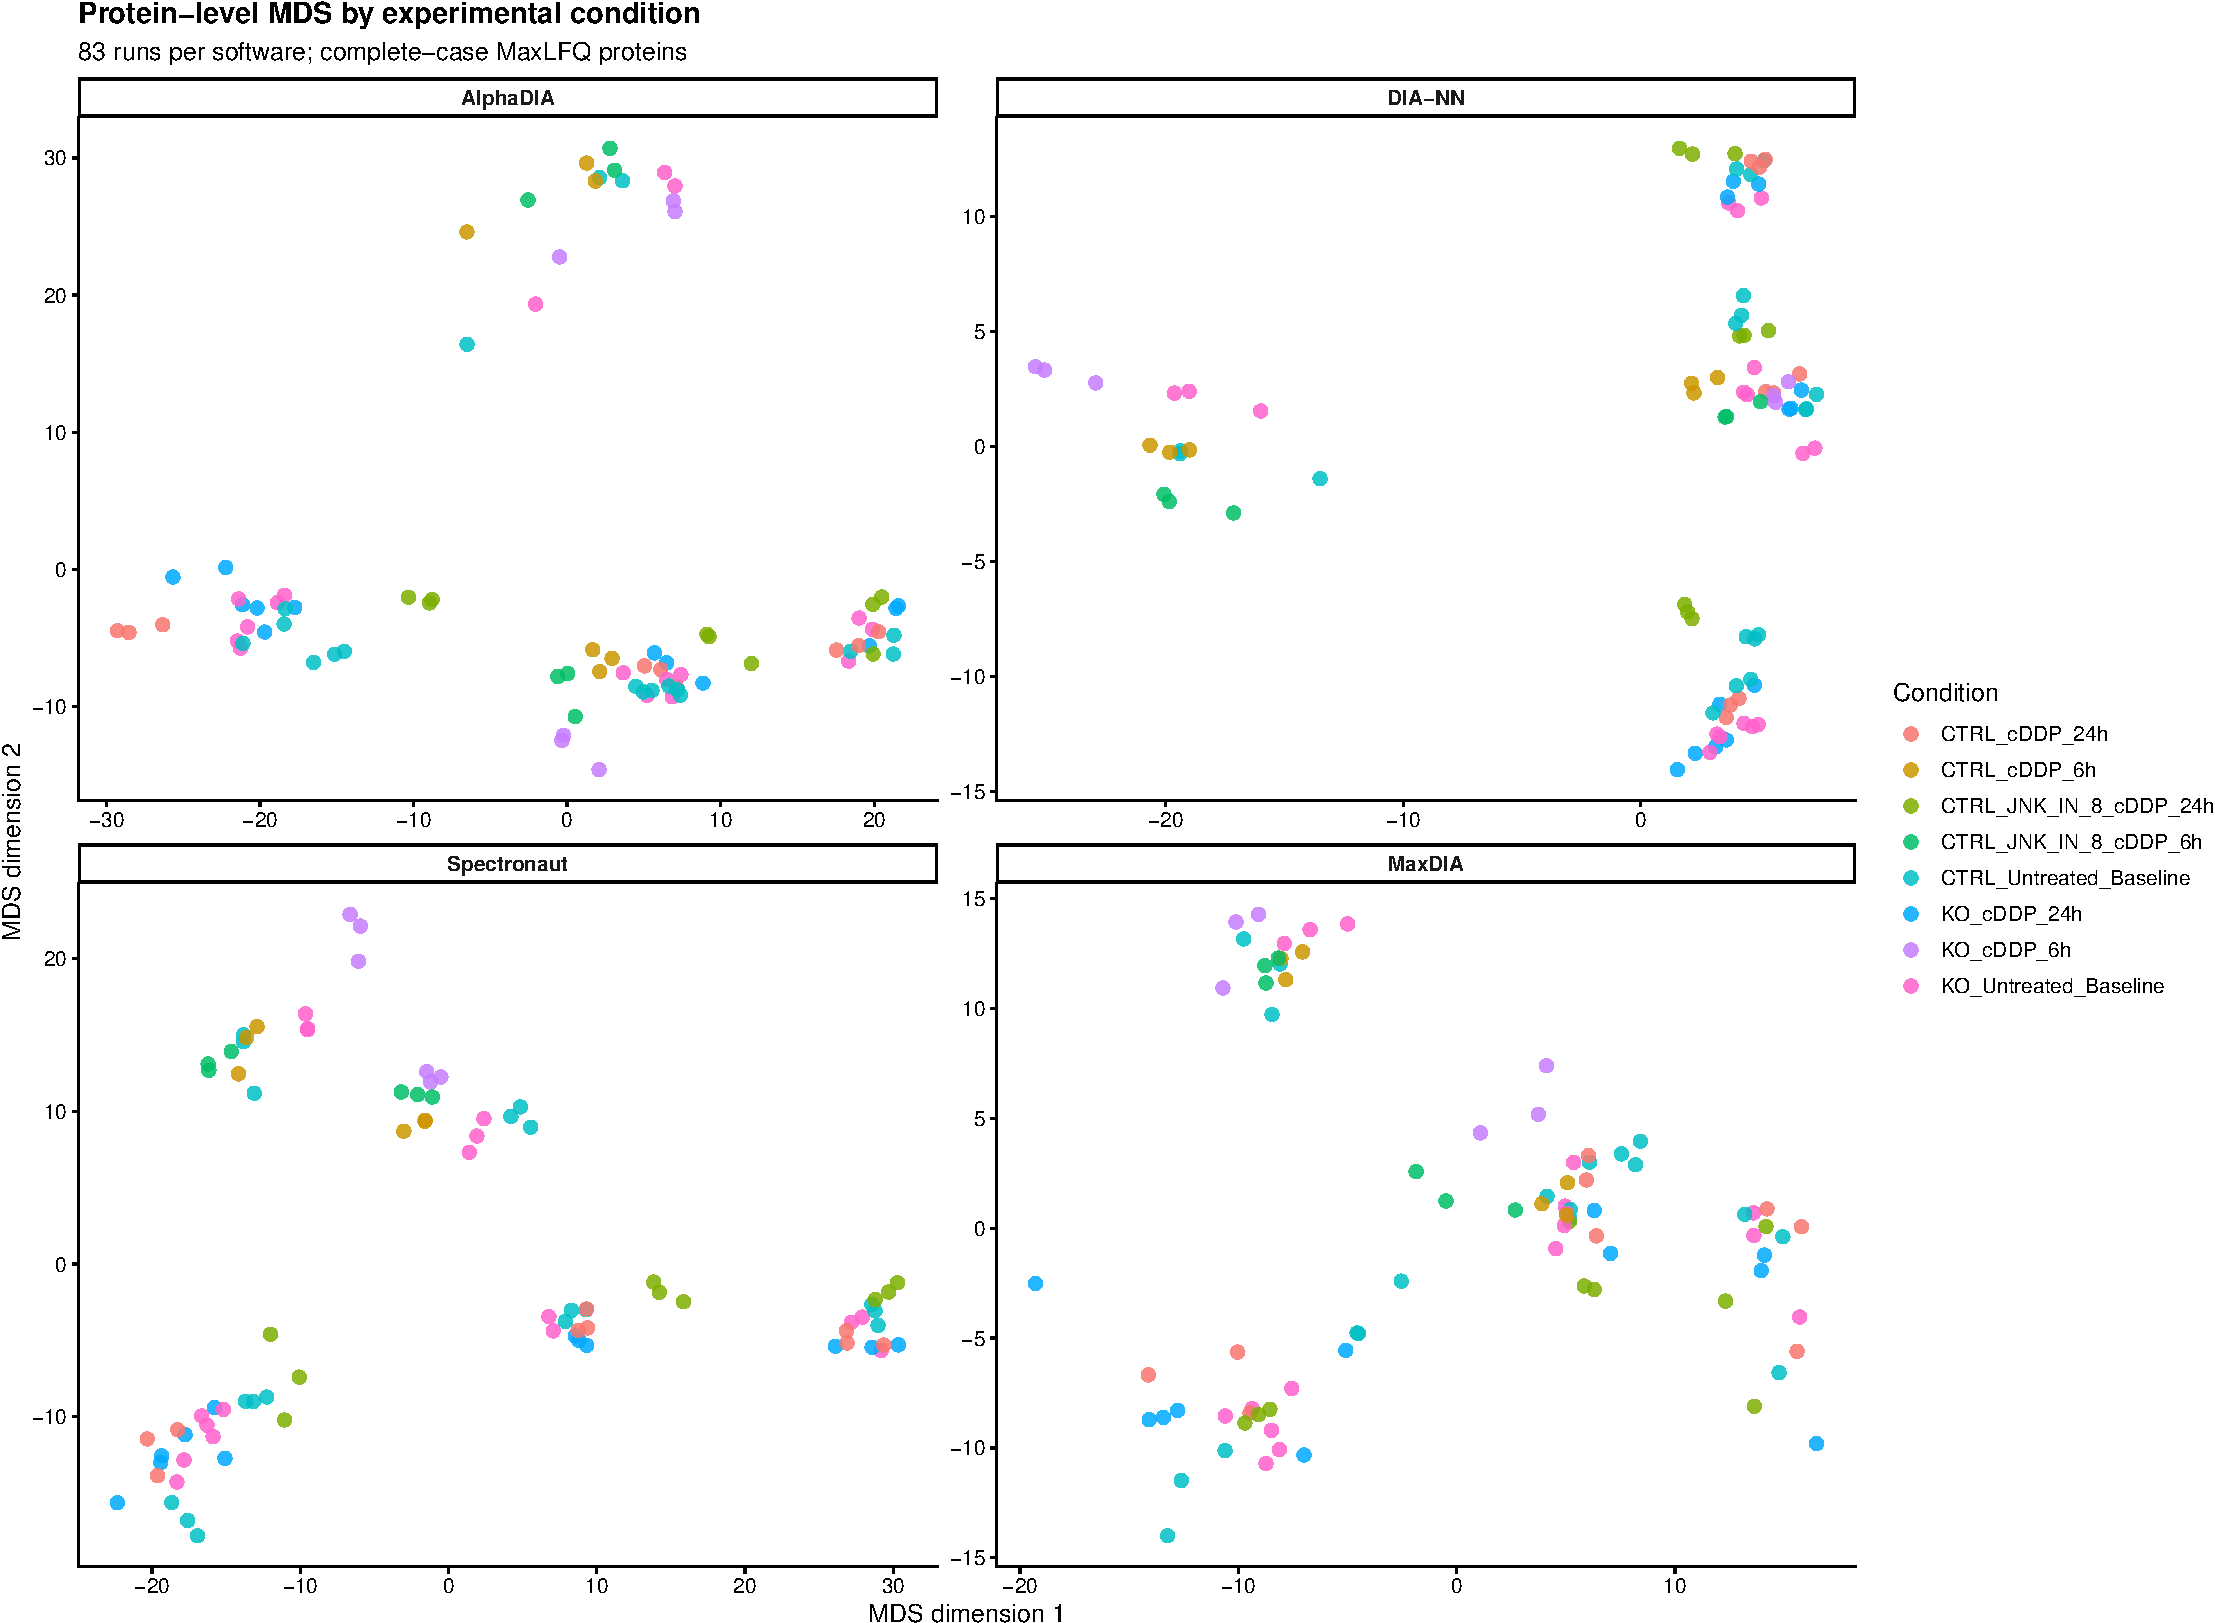
\includegraphics[width=1\linewidth]{DIA_CapstoneProject2026_files/figure-latex/protein_mds_qc-1} \end{center}

\begin{center}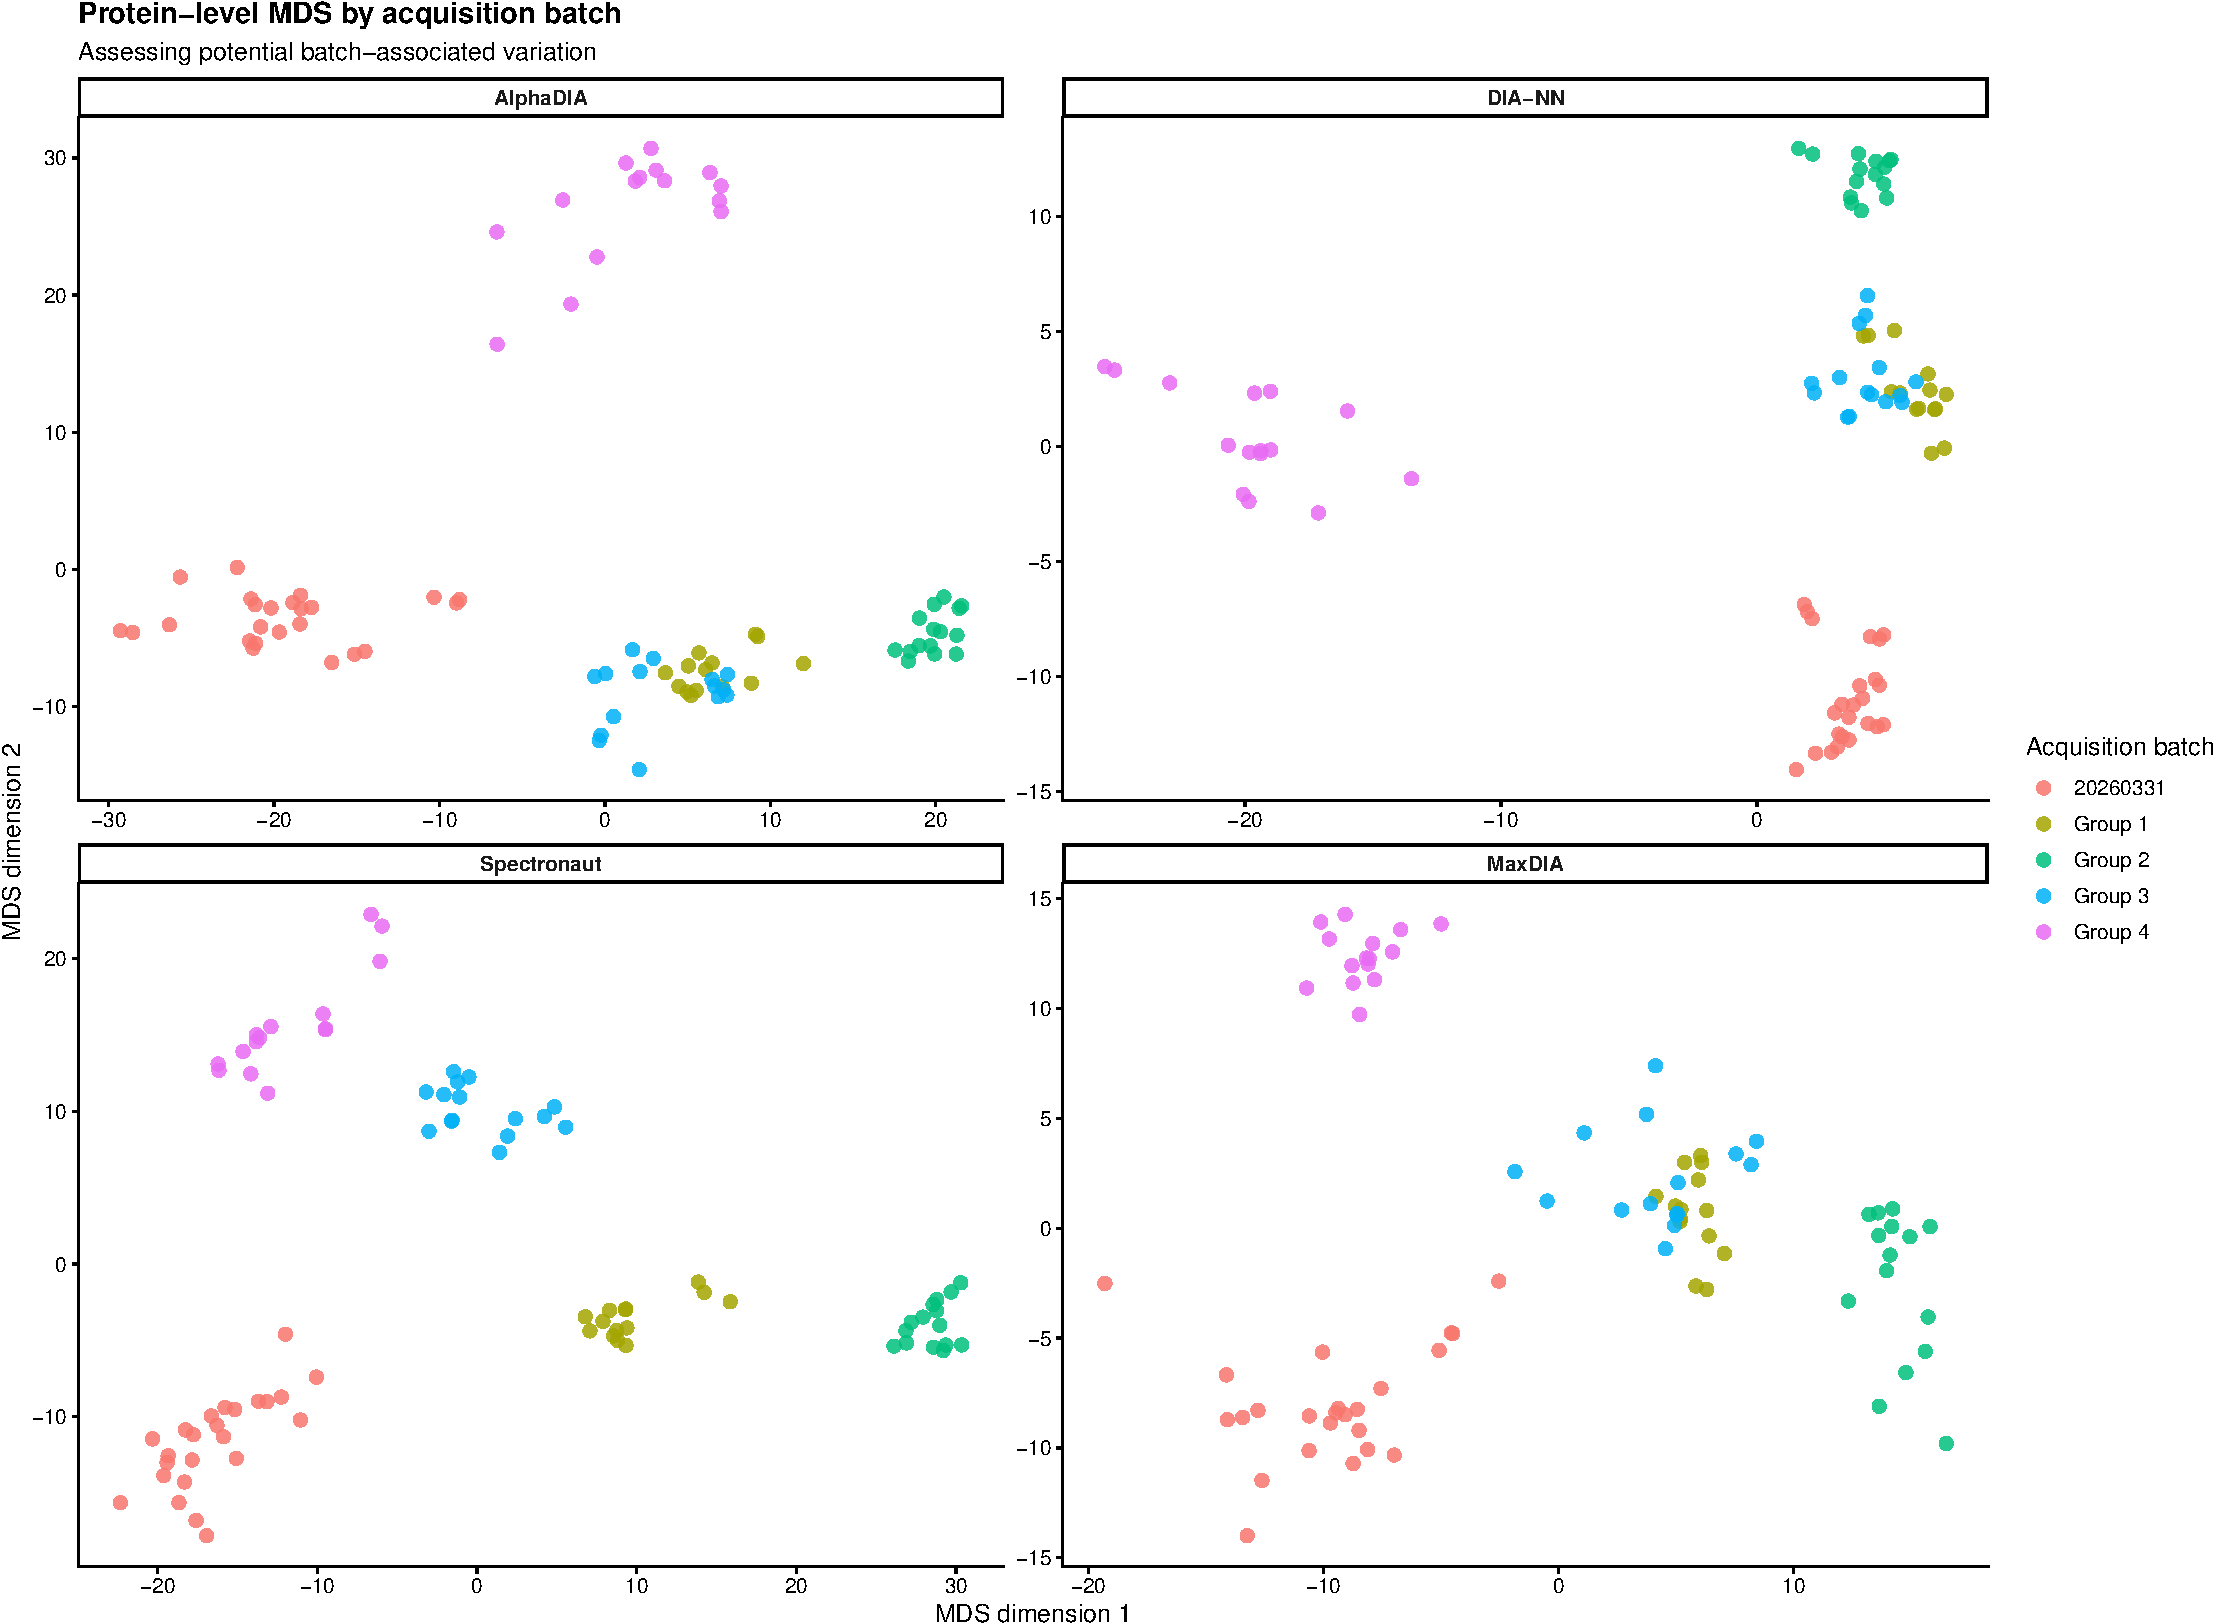
\includegraphics[width=1\linewidth]{DIA_CapstoneProject2026_files/figure-latex/protein_mds_qc-2} \end{center}

The MDS plots reveal a strong acquisition batch effect across all four
DIA software pipelines, with substantially weaker separation by
biological condition. This is an important finding before statistical
modeling. 1. MDS by experimental condition Samples form several distinct
clusters in AlphaDIA, DIA-NN, Spectronaut, and MaxDIA. However, these
clusters contain mixtures of experimental conditions rather than showing
clear separation by genotype or treatment. Some conditions are
distributed across multiple clusters, suggesting that experimental
condition is not the dominant source of variation in the first two MDS
dimensions. MaxDIA also shows somewhat greater dispersion within
clusters. 2. MDS by acquisition batch The batch-colored plots show
pronounced clustering according to acquisition batch in all four
pipelines. AlphaDIA, DIA-NN, and Spectronaut exhibit particularly clear
batch separation, while MaxDIA shows a similar pattern with slightly
greater within-batch variability. Importantly, these patterns persist
despite Median of Ratios normalization, indicating that global intensity
normalization has not eliminated batch-associated variation.

These are substantial numbers of proteins for exploratory MDS, although
each software uses a different set of complete-case proteins.

The results suggest that acquisition batch is a major source of
protein-level variation, potentially masking biological differences
between experimental conditions. This is consistent across all four
analysis pipelines and therefore deserves attention before differential
abundance analysis.

\begin{verbatim}
## # A tibble: 8 x 7
##   Condition           `Group 1` `Group 2` `Group 3` `Group 4` `20260331` Unknown
##   <chr>                   <int>     <int>     <int>     <int>      <int>   <int>
## 1 CTRL_JNK_IN_8_cDDP~         3         3         0         0          3       0
## 2 CTRL_JNK_IN_8_cDDP~         0         0         3         3          0       0
## 3 CTRL_Untreated_Bas~         3         3         3         3          6       0
## 4 CTRL_cDDP_24h               3         3         0         0          3       0
## 5 CTRL_cDDP_6h                0         0         3         3          0       0
## 6 KO_Untreated_Basel~         2         3         3         3          6       0
## 7 KO_cDDP_24h                 3         3         0         0          6       0
## 8 KO_cDDP_6h                  0         0         3         3          0       0
\end{verbatim}

\begin{verbatim}
## # A tibble: 8 x 3
##   Condition               Total_Runs Batches_Represented
##   <chr>                        <int>               <int>
## 1 CTRL_JNK_IN_8_cDDP_24h           9                   3
## 2 CTRL_JNK_IN_8_cDDP_6h            6                   2
## 3 CTRL_Untreated_Baseline         18                   5
## 4 CTRL_cDDP_24h                    9                   3
## 5 CTRL_cDDP_6h                     6                   2
## 6 KO_Untreated_Baseline           17                   5
## 7 KO_cDDP_24h                     12                   3
## 8 KO_cDDP_6h                       6                   2
\end{verbatim}

\begin{center}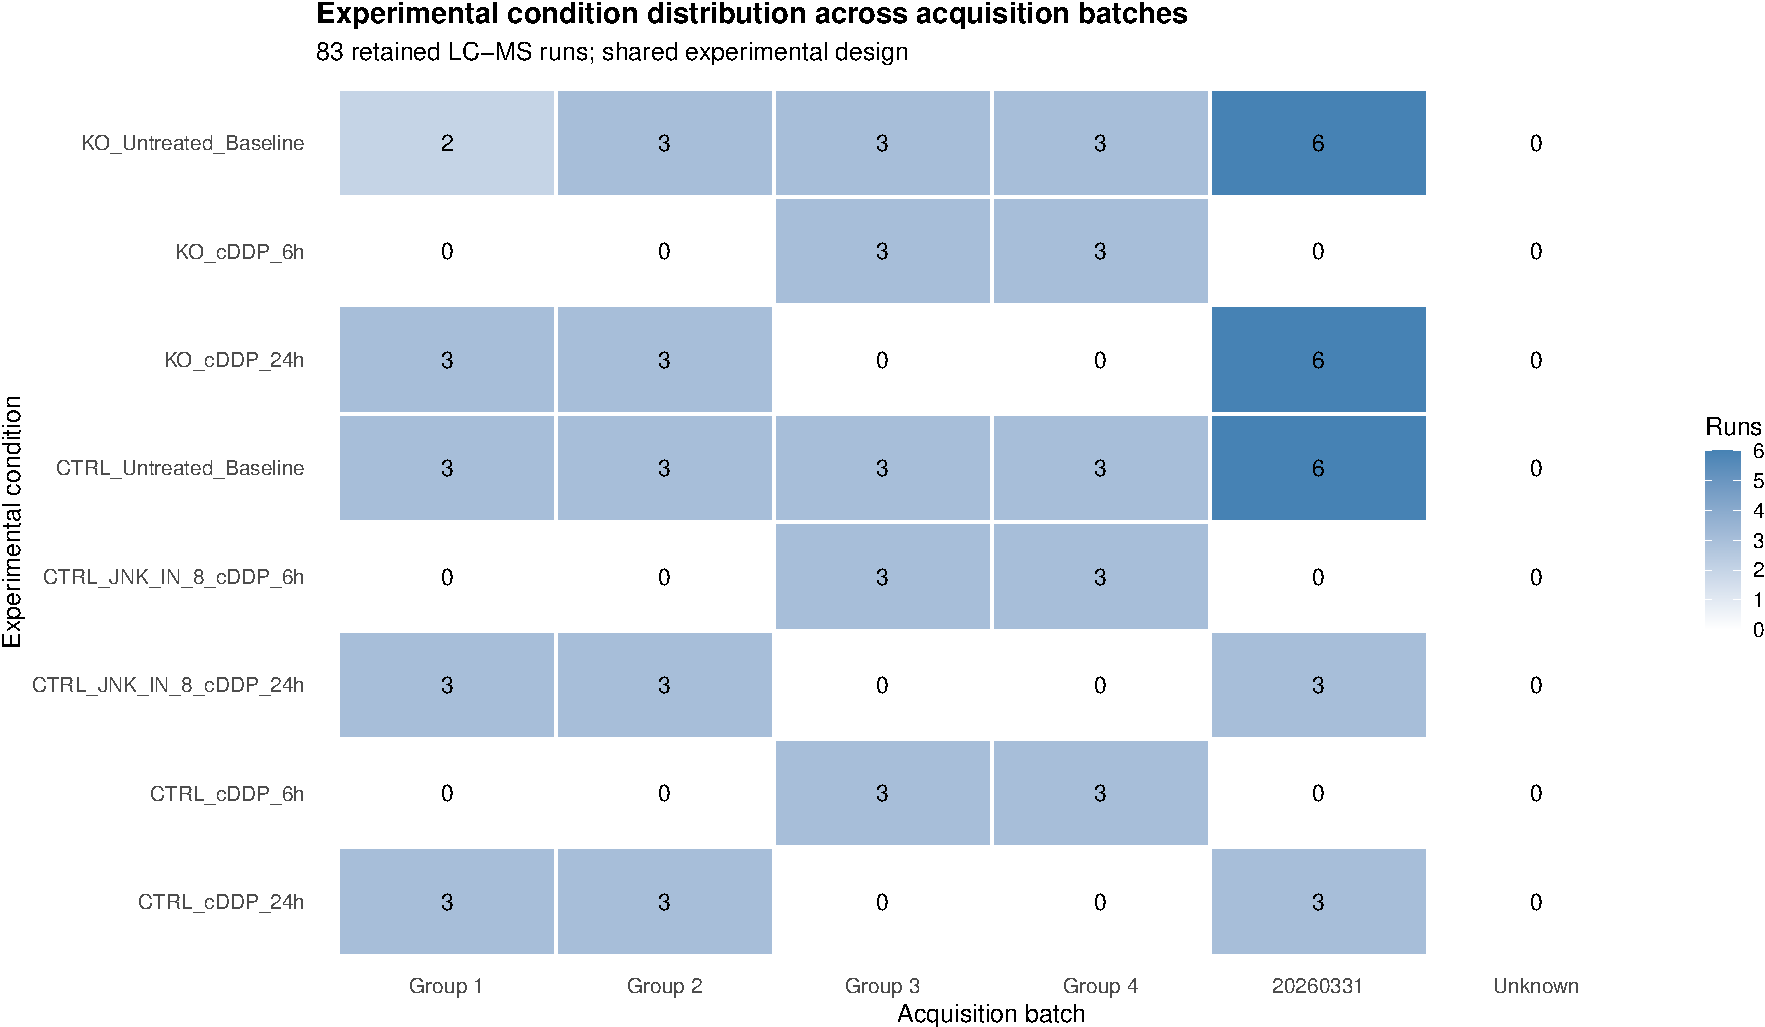
\includegraphics[width=1\linewidth]{DIA_CapstoneProject2026_files/figure-latex/qc_condition_batch_balance-1} \end{center}

The key findings are: - Untreated controls and KO samples are
represented across all five acquisition batches, providing useful
reference groups. - 24-hour cisplatin treatments are represented in
Groups 1--2 and the 20260331 batch, whereas 6-hour treatments occur
exclusively in Groups 3--4. - JNK inhibitor treatments follow the same
time-dependent batch allocation. - Every experimental condition appears
in at least two batches, but the design is not fully crossed. Most
importantly, treatment duration (6 h versus 24 h) is confounded with
acquisition batch among treated samples. Consequently, a direct
comparison of 6-hour and 24-hour treatment effects cannot be reliably
separated from batch effects without additional assumptions.

\subsection{Correlation matrix}\label{correlation-matrix}

\begin{verbatim}
##      Software Median_Within_Batch Median_Between_Batch Minimum_Correlation
## 1    AlphaDIA           0.9224902            0.8388438           0.6675239
## 2      DIA-NN           0.9855453            0.9740804           0.9382949
## 3 Spectronaut           0.8988642            0.8058905           0.5927934
## 4      MaxDIA           0.7846717            0.7219390           0.5213387
##   Median_Correlation
## 1          0.8506624
## 2          0.9756171
## 3          0.8169630
## 4          0.7307202
\end{verbatim}

\begin{center}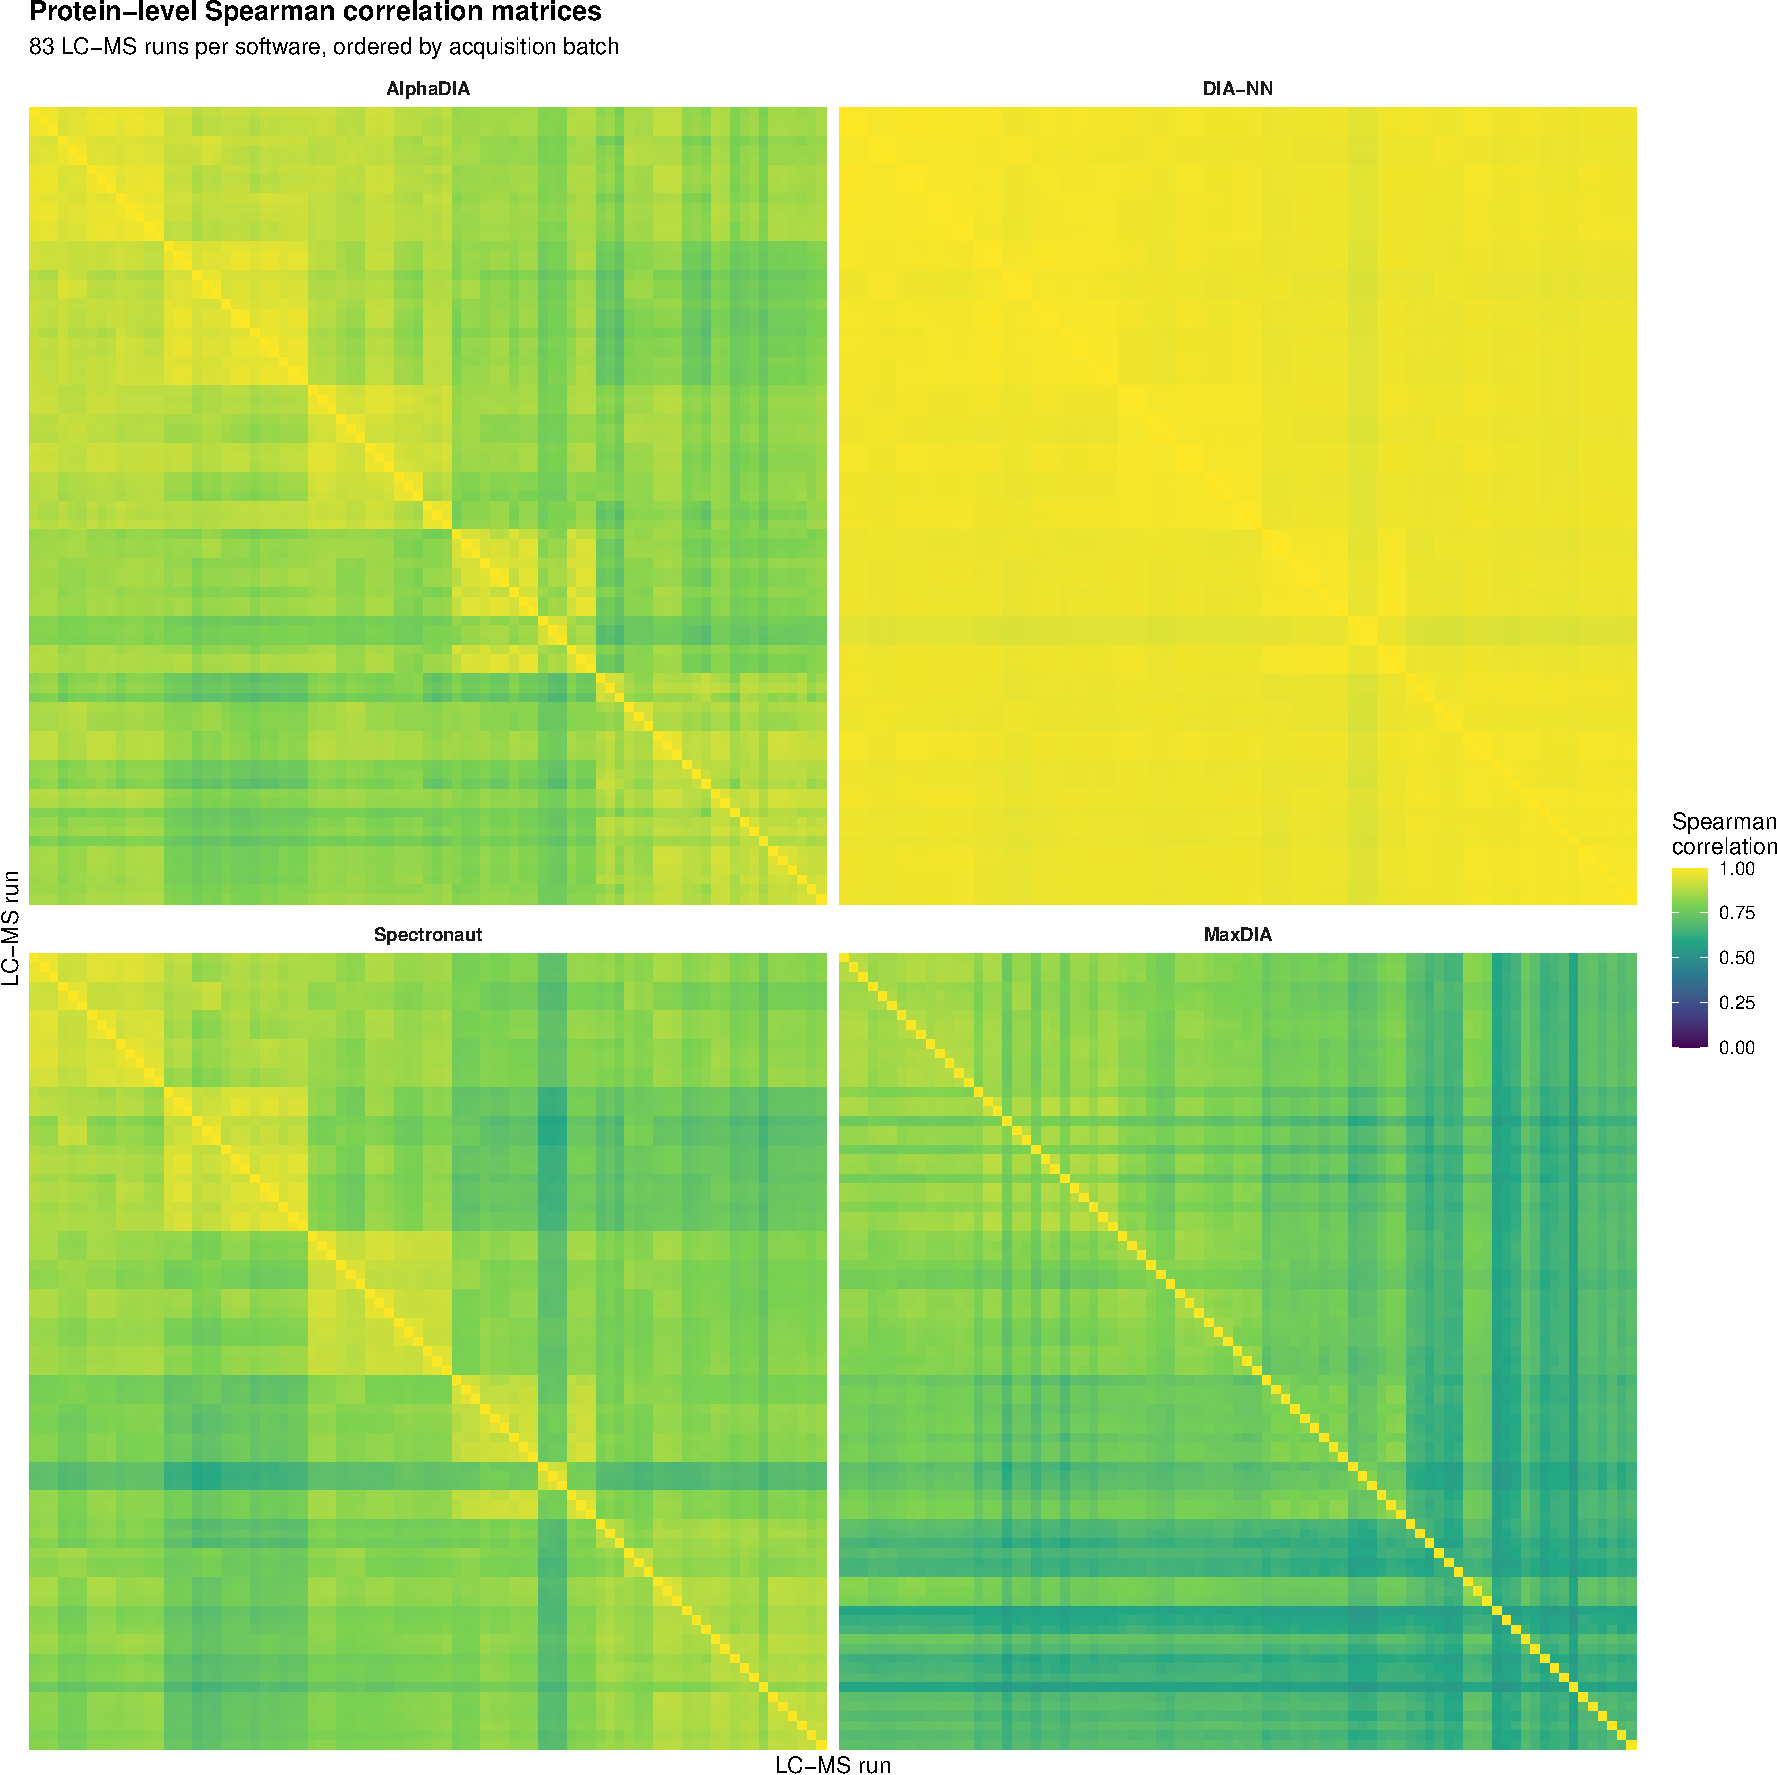
\includegraphics[width=1\linewidth]{DIA_CapstoneProject2026_files/figure-latex/qc_protein_spearman_correlation-1} \end{center}

The correlation matrices reveal high overall protein-level similarity
between samples, but clear software-dependent differences and
batch-associated variation. DIA-NN exhibits the strongest correlations
(median 0.976), with only a small difference between within-batch
(0.986) and between-batch (0.974) correlations, indicating highly
consistent protein abundance rankings across runs. AlphaDIA and
Spectronaut show good overall correlations (medians 0.851 and 0.817),
but noticeably higher within-batch than between-batch similarity
(differences of 0.084 and 0.093, respectively), supporting the batch
effects observed in MDS. MaxDIA displays the lowest overall correlation
(median 0.731), the lowest minimum correlation (0.521), and greater
sample-to-sample variability. Overall, these findings reinforce the
importance of accounting for acquisition batch during differential
abundance modeling, particularly for AlphaDIA, Spectronaut, and MaxDIA.

\section{Data modeling}\label{data-modeling}

The experimental design also shows that 6-hour treatments were acquired
in Groups 3--4, while 24-hour treatments were acquired in Groups 1--2
and 20260331. This means direct 6-hour versus 24-hour comparisons are
particularly vulnerable to batch confounding. However, comparisons such
as KO versus CTRL within the same treatment and time point are better
supported because those conditions share acquisition batches.

Here, condition represents your eight biological experimental groups,
while Batch accounts for systematic differences between the five
acquisition batches.

\subsection{Construct and evaluate the design
matrix}\label{construct-and-evaluate-the-design-matrix}

\begin{verbatim}
##   Runs Parameters Rank Full_Rank Residual_DF
## 1   83         12   12      TRUE          71
\end{verbatim}

\begin{verbatim}
## 
## Design matrix columns:
\end{verbatim}

\begin{verbatim}
##  [1] "(Intercept)"                     "BatchGroup2"                    
##  [3] "BatchGroup3"                     "BatchGroup4"                    
##  [5] "Batch20260331"                   "conditionKO_Untreated_Baseline" 
##  [7] "conditionCTRL_cDDP_6h"           "conditionKO_cDDP_6h"            
##  [9] "conditionCTRL_JNK_IN_8_cDDP_6h"  "conditionCTRL_cDDP_24h"         
## [11] "conditionKO_cDDP_24h"            "conditionCTRL_JNK_IN_8_cDDP_24h"
\end{verbatim}

\begin{verbatim}
## 
## Condition by batch:
\end{verbatim}

\begin{verbatim}
##                          
##                           Group1 Group2 Group3 Group4 20260331
##   CTRL_Untreated_Baseline      3      3      3      3        6
##   KO_Untreated_Baseline        2      3      3      3        6
##   CTRL_cDDP_6h                 0      0      3      3        0
##   KO_cDDP_6h                   0      0      3      3        0
##   CTRL_JNK_IN_8_cDDP_6h        0      0      3      3        0
##   CTRL_cDDP_24h                3      3      0      0        3
##   KO_cDDP_24h                  3      3      0      0        6
##   CTRL_JNK_IN_8_cDDP_24h       3      3      0      0        3
\end{verbatim}

\begin{verbatim}
## 
## Design matrix is full rank.
\end{verbatim}

\subsection{Evaluate biologically relevant
contrasts}\label{evaluate-biologically-relevant-contrasts}

The most informative comparisons include genotype effects, cisplatin
treatment effects, and the effect of adding JNK-IN-8 to
cisplatin-treated CTRL samples. We can test whether these contrasts are
estimable under the batch-adjusted model and whether the compared
conditions share acquisition batches.

\begin{verbatim}
##                        Contrast Estimable Shared_Batches
##             KO vs CTRL baseline      TRUE              5
##         KO vs CTRL cisplatin 6h      TRUE              2
##        KO vs CTRL cisplatin 24h      TRUE              3
##   CTRL cisplatin 6h vs baseline      TRUE              2
##  CTRL cisplatin 24h vs baseline      TRUE              3
##     KO cisplatin 6h vs baseline      TRUE              2
##    KO cisplatin 24h vs baseline      TRUE              3
##      JNK inhibitor effect at 6h      TRUE              2
##     JNK inhibitor effect at 24h      TRUE              3
##        CTRL cisplatin 24h vs 6h      TRUE              0
##          KO cisplatin 24h vs 6h      TRUE              0
##                               Batch_Names
##  20260331, Group1, Group2, Group3, Group4
##                            Group3, Group4
##                  20260331, Group1, Group2
##                            Group3, Group4
##                  20260331, Group1, Group2
##                            Group3, Group4
##                  20260331, Group1, Group2
##                            Group3, Group4
##                  20260331, Group1, Group2
##                                      None
##                                      None
\end{verbatim}

Nine of the eleven contrasts have direct within-batch support. These
should be the primary focus of your differential abundance analysis.

The two 24 h versus 6 h comparisons are mathematically estimable but
have no shared acquisition batches. Their estimates depend on the
additive batch-effect assumption and the untreated samples that connect
batches. I recommend treating these as exploratory rather than primary
contrasts.

Although the overall design supports these contrasts, individual
proteins may have missing observations. A protein measured only in
certain batches or conditions may not support every contrast, even when
the overall design matrix is full rank. \#\# Protein-level missingness
and contrast-specific data availability

\begin{verbatim}
##      Software Total_Proteins Runs Complete_Proteins Complete_Percent
## 1    AlphaDIA          11331   83              8828         77.91016
## 2      DIA-NN           9833   83              7557         76.85345
## 3 Spectronaut           7970   83              7581         95.11920
## 4      MaxDIA           8482   83              7515         88.59939
##   Median_Detected_Runs Proteins_At_Least_Half_Runs
## 1                   83                       11156
## 2                   83                        9529
## 3                   83                        7968
## 4                   83                        8478
\end{verbatim}

\begin{verbatim}
##     Software                       Contrast Both_Groups_At_Least_2
##     AlphaDIA            KO vs CTRL baseline                  11326
##     AlphaDIA        KO vs CTRL cisplatin 6h                  11164
##     AlphaDIA       KO vs CTRL cisplatin 24h                  11299
##     AlphaDIA  CTRL cisplatin 6h vs baseline                  11246
##     AlphaDIA CTRL cisplatin 24h vs baseline                  11310
##     AlphaDIA    KO cisplatin 6h vs baseline                  11207
##     AlphaDIA   KO cisplatin 24h vs baseline                  11311
##     AlphaDIA     JNK inhibitor effect at 6h                  11173
##     AlphaDIA    JNK inhibitor effect at 24h                  11287
##     AlphaDIA       CTRL cisplatin 24h vs 6h                  11236
##     AlphaDIA         KO cisplatin 24h vs 6h                  11197
##       DIA-NN            KO vs CTRL baseline                   9815
##       DIA-NN        KO vs CTRL cisplatin 6h                   9627
##       DIA-NN       KO vs CTRL cisplatin 24h                   9749
##       DIA-NN  CTRL cisplatin 6h vs baseline                   9736
##       DIA-NN CTRL cisplatin 24h vs baseline                   9789
##       DIA-NN    KO cisplatin 6h vs baseline                   9668
##       DIA-NN   KO cisplatin 24h vs baseline                   9759
##       DIA-NN     JNK inhibitor effect at 6h                   9662
##       DIA-NN    JNK inhibitor effect at 24h                   9752
##       DIA-NN       CTRL cisplatin 24h vs 6h                   9708
##       DIA-NN         KO cisplatin 24h vs 6h                   9630
##  Spectronaut            KO vs CTRL baseline                   7970
##  Spectronaut        KO vs CTRL cisplatin 6h                   7969
##  Spectronaut       KO vs CTRL cisplatin 24h                   7969
##  Spectronaut  CTRL cisplatin 6h vs baseline                   7969
##  Spectronaut CTRL cisplatin 24h vs baseline                   7969
##  Spectronaut    KO cisplatin 6h vs baseline                   7970
##  Spectronaut   KO cisplatin 24h vs baseline                   7970
##  Spectronaut     JNK inhibitor effect at 6h                   7967
##  Spectronaut    JNK inhibitor effect at 24h                   7969
##  Spectronaut       CTRL cisplatin 24h vs 6h                   7968
##  Spectronaut         KO cisplatin 24h vs 6h                   7970
##       MaxDIA            KO vs CTRL baseline                   8481
##       MaxDIA        KO vs CTRL cisplatin 6h                   8477
##       MaxDIA       KO vs CTRL cisplatin 24h                   8480
##       MaxDIA  CTRL cisplatin 6h vs baseline                   8479
##       MaxDIA CTRL cisplatin 24h vs baseline                   8480
##       MaxDIA    KO cisplatin 6h vs baseline                   8479
##       MaxDIA   KO cisplatin 24h vs baseline                   8480
##       MaxDIA     JNK inhibitor effect at 6h                   8478
##       MaxDIA    JNK inhibitor effect at 24h                   8480
##       MaxDIA       CTRL cisplatin 24h vs 6h                   8478
##       MaxDIA         KO cisplatin 24h vs 6h                   8478
##  Both_Groups_Percent Shared_Batch_Support Both_And_Shared_Batch
##             99.95587                11326                 11325
##             98.52617                11240                 11162
##             99.71759                11319                 11299
##             99.24985                11270                 11236
##             99.81467                11317                 11307
##             98.90566                11248                 11195
##             99.82349                11315                 11307
##             98.60560                11242                 11167
##             99.61168                11309                 11287
##             99.16159                    0                     0
##             98.81740                    0                     0
##             99.81694                 9824                  9815
##             97.90501                 9729                  9625
##             99.14573                 9788                  9747
##             99.01353                 9759                  9715
##             99.55253                 9805                  9787
##             98.32198                 9716                  9646
##             99.24743                 9785                  9756
##             98.26096                 9743                  9655
##             99.17624                 9791                  9751
##             98.72877                    0                     0
##             97.93552                    0                     0
##            100.00000                 7970                  7970
##             99.98745                 7970                  7969
##             99.98745                 7969                  7969
##             99.98745                 7970                  7969
##             99.98745                 7969                  7969
##            100.00000                 7970                  7970
##            100.00000                 7970                  7970
##             99.96236                 7970                  7967
##             99.98745                 7968                  7968
##             99.97491                    0                     0
##            100.00000                    0                     0
##             99.98821                 8481                  8481
##             99.94105                 8479                  8477
##             99.97642                 8480                  8480
##             99.96463                 8481                  8479
##             99.97642                 8480                  8480
##             99.96463                 8480                  8479
##             99.97642                 8479                  8479
##             99.95284                 8479                  8478
##             99.97642                 8480                  8480
##             99.95284                    0                     0
##             99.95284                    0                     0
\end{verbatim}

These are strong protein-level completeness results across all four
pipelines.

A few observations: - AlphaDIA quantifies the largest number of
proteins. - Spectronaut has the highest completeness (95.1\%), although
its previously observed low-intensity reporting floor remains a caveat.
- MaxDIA shows considerably better completeness at protein level than at
precursor level, consistent with MaxLFQ aggregation combining
information across precursors. - All four tools have a median detection
frequency of 83 runs, meaning at least half their proteins are
quantified in every sample. Importantly, MaxLFQ protein aggregation has
substantially reduced the missingness observed at precursor level.

Protein-level missingness is unlikely to be a major limitation for
differential abundance analysis across the four DIA pipelines. Across
all 11 planned comparisons, the percentage of proteins quantified in at
least two samples in both conditions is: Software Range across contrasts
Interpretation AlphaDIA 98.5--100\% Excellent availability DIA-NN
97.9--99.8\% Excellent availability Spectronaut 99.96--100\% Nearly
complete MaxDIA 99.94--99.99\% Nearly complete

This is particularly reassuring because the 6-hour treatment groups
contain only six replicates each.

Although the 6 h and 24 h conditions do not share batches, untreated
samples connect the groups statistically. Therefore, their contrasts can
be estimable under the additive model. But they rely more strongly on
assumptions about batch effects. I recommend keeping these two time
comparisons as exploratory analyses.

In other word, Protein-level data availability was high across all four
DIA analysis pipelines. Between 97.9\% and 100\% of quantified proteins
had at least two observations in each condition for the planned
contrasts. Nine of the eleven comparisons had direct within-batch
support, whereas comparisons between 6-hour and 24-hour cisplatin
treatments lacked overlapping acquisition batches. Although these
time-point contrasts were mathematically estimable under the additive
batch-adjusted design, their interpretation requires caution because
treatment duration and acquisition batch were partially confounded.
Overall, the results support proceeding with batch-adjusted differential
abundance modeling without additional global completeness filtering.

\begin{verbatim}
## Checking: AlphaDIA 
## Checking: DIA-NN 
## Checking: Spectronaut 
## Checking: MaxDIA
\end{verbatim}

\begin{verbatim}
## 
## Protein-specific design rank:
\end{verbatim}

\begin{verbatim}
##     Software Total_Proteins Unique_Missingness_Patterns Full_Rank_Proteins
##     AlphaDIA          11331                        2018              11109
##       DIA-NN           9833                        1917               9607
##  Spectronaut           7970                         308               7969
##       MaxDIA           8482                         556               8476
##  Full_Rank_Percent Median_Protein_Rank
##           98.04077                  12
##           97.70162                  12
##           99.98745                  12
##           99.92926                  12
\end{verbatim}

\begin{verbatim}
## 
## Protein-specific contrast estimability:
\end{verbatim}

\begin{verbatim}
##     Software                       Contrast Estimable_Proteins Total_Proteins
##     AlphaDIA            KO vs CTRL baseline              11326          11331
##     AlphaDIA        KO vs CTRL cisplatin 6h              11251          11331
##     AlphaDIA       KO vs CTRL cisplatin 24h              11319          11331
##     AlphaDIA  CTRL cisplatin 6h vs baseline              11283          11331
##     AlphaDIA CTRL cisplatin 24h vs baseline              11323          11331
##     AlphaDIA    KO cisplatin 6h vs baseline              11266          11331
##     AlphaDIA   KO cisplatin 24h vs baseline              11321          11331
##     AlphaDIA     JNK inhibitor effect at 6h              11252          11331
##     AlphaDIA    JNK inhibitor effect at 24h              11314          11331
##     AlphaDIA       CTRL cisplatin 24h vs 6h              11279          11331
##     AlphaDIA         KO cisplatin 24h vs 6h              11261          11331
##       DIA-NN            KO vs CTRL baseline               9824           9833
##       DIA-NN        KO vs CTRL cisplatin 6h               9739           9833
##       DIA-NN       KO vs CTRL cisplatin 24h               9795           9833
##       DIA-NN  CTRL cisplatin 6h vs baseline               9792           9833
##       DIA-NN CTRL cisplatin 24h vs baseline               9813           9833
##       DIA-NN    KO cisplatin 6h vs baseline               9750           9833
##       DIA-NN   KO cisplatin 24h vs baseline               9796           9833
##       DIA-NN     JNK inhibitor effect at 6h               9762           9833
##       DIA-NN    JNK inhibitor effect at 24h               9801           9833
##       DIA-NN       CTRL cisplatin 24h vs 6h               9777           9833
##       DIA-NN         KO cisplatin 24h vs 6h               9729           9833
##  Spectronaut            KO vs CTRL baseline               7970           7970
##  Spectronaut        KO vs CTRL cisplatin 6h               7970           7970
##  Spectronaut       KO vs CTRL cisplatin 24h               7969           7970
##  Spectronaut  CTRL cisplatin 6h vs baseline               7970           7970
##  Spectronaut CTRL cisplatin 24h vs baseline               7969           7970
##  Spectronaut    KO cisplatin 6h vs baseline               7970           7970
##  Spectronaut   KO cisplatin 24h vs baseline               7970           7970
##  Spectronaut     JNK inhibitor effect at 6h               7970           7970
##  Spectronaut    JNK inhibitor effect at 24h               7969           7970
##  Spectronaut       CTRL cisplatin 24h vs 6h               7969           7970
##  Spectronaut         KO cisplatin 24h vs 6h               7970           7970
##       MaxDIA            KO vs CTRL baseline               8481           8482
##       MaxDIA        KO vs CTRL cisplatin 6h               8480           8482
##       MaxDIA       KO vs CTRL cisplatin 24h               8480           8482
##       MaxDIA  CTRL cisplatin 6h vs baseline               8481           8482
##       MaxDIA CTRL cisplatin 24h vs baseline               8480           8482
##       MaxDIA    KO cisplatin 6h vs baseline               8480           8482
##       MaxDIA   KO cisplatin 24h vs baseline               8480           8482
##       MaxDIA     JNK inhibitor effect at 6h               8480           8482
##       MaxDIA    JNK inhibitor effect at 24h               8480           8482
##       MaxDIA       CTRL cisplatin 24h vs 6h               8479           8482
##       MaxDIA         KO cisplatin 24h vs 6h               8479           8482
##  Estimable_Percent
##           99.95587
##           99.29397
##           99.89410
##           99.57638
##           99.92940
##           99.42635
##           99.91175
##           99.30280
##           99.84997
##           99.54108
##           99.38223
##           99.90847
##           99.04404
##           99.61355
##           99.58304
##           99.79660
##           99.15590
##           99.62372
##           99.27794
##           99.67457
##           99.43049
##           98.94234
##          100.00000
##          100.00000
##           99.98745
##          100.00000
##           99.98745
##          100.00000
##          100.00000
##          100.00000
##           99.98745
##           99.98745
##          100.00000
##           99.98821
##           99.97642
##           99.97642
##           99.98821
##           99.97642
##           99.97642
##           99.97642
##           99.97642
##           99.97642
##           99.96463
##           99.96463
\end{verbatim}

The median protein-specific design rank is 12 for every software
pipeline, matching the number of model coefficients. This means that
nearly all proteins have sufficient observations across the experimental
conditions and acquisition batches to estimate every coefficient in the
proposed model. Importantly, the remaining rank-deficient proteins are
not necessarily unusable. Some can still support particular biological
contrasts. Protein-specific design matrix diagnostics demonstrated high
model identifiability across all four DIA analysis pipelines. Full-rank
design matrices were obtained for 98.04\% of AlphaDIA proteins, 97.70\%
of DIA-NN proteins, 99.99\% of Spectronaut proteins, and 99.93\% of
MaxDIA proteins. Across the eleven planned biological contrasts,
mathematical estimability exceeded 98.9\% for every pipeline. These
findings indicate that protein-level missingness is unlikely to
substantially restrict differential abundance analysis. Nevertheless,
direct comparisons between 6-hour and 24-hour cisplatin treatments
remain dependent on additive batch-effect assumptions because the
treatment groups were acquired in separate batches. Therefore,
subsequent statistical modeling will incorporate acquisition batch as a
fixed effect, with cross-time-point comparisons interpreted cautiously.

\subsection{Statistical inference}\label{statistical-inference}

This chunk will: - Add the acquisition batch annotation to the colData
of all four QFeatures objects. - Standardize condition and Batch factor
levels. - Check that the 83 runs align correctly. - Verify that each
software produces the same full-rank design matrix. - Leave all
abundance values and existing assays unchanged.

\begin{verbatim}
##     Software Runs Parameters Rank Full_Rank Missing_Metadata
##     AlphaDIA   83         12   12      TRUE                0
##       DIA-NN   83         12   12      TRUE                0
##  Spectronaut   83         12   12      TRUE                0
##       MaxDIA   83         12   12      TRUE                0
\end{verbatim}

\subsubsection{Fit the first protein-level
model}\label{fit-the-first-protein-level-model}

These results are encouraging. All four DIA pipelines have successfully
produced robust models for the overwhelming majority of proteins, but a
small subset requires caution before differential abundance testing. The
median residual degrees of freedom are approximately 66 across all four
pipelines, suggesting that most models retain substantial information
after accounting for batch and condition.

We now have all 11 planned biological contrasts, and their condition
names match your batch-adjusted model. We'll preserve the direction of
each comparison: log2 fold change = Numerator − Denominator For example,
a positive log2FC for KO vs CTRL cisplatin 6h means higher protein
abundance in KO than CTRL at 6h.

\subsubsection{Construct the contrast
matrix}\label{construct-the-contrast-matrix}

\begin{verbatim}
## Contrast matrix dimensions: 12 11
\end{verbatim}

\begin{verbatim}
##                                  KO vs CTRL baseline KO vs CTRL cisplatin 6h
## (Intercept)                                        0                       0
## BatchGroup2                                        0                       0
## BatchGroup3                                        0                       0
## BatchGroup4                                        0                       0
## Batch20260331                                      0                       0
## conditionCTRL_cDDP_6h                              0                      -1
## conditionCTRL_JNK_IN_8_cDDP_24h                    0                       0
## conditionCTRL_JNK_IN_8_cDDP_6h                     0                       0
## conditionCTRL_Untreated_Baseline                  -1                       0
## conditionKO_cDDP_24h                               0                       0
## conditionKO_cDDP_6h                                0                       1
## conditionKO_Untreated_Baseline                     1                       0
##                                  KO vs CTRL cisplatin 24h
## (Intercept)                                             0
## BatchGroup2                                             0
## BatchGroup3                                             0
## BatchGroup4                                             0
## Batch20260331                                           0
## conditionCTRL_cDDP_6h                                   0
## conditionCTRL_JNK_IN_8_cDDP_24h                         0
## conditionCTRL_JNK_IN_8_cDDP_6h                          0
## conditionCTRL_Untreated_Baseline                        0
## conditionKO_cDDP_24h                                    1
## conditionKO_cDDP_6h                                     0
## conditionKO_Untreated_Baseline                          0
##                                  CTRL cisplatin 6h vs baseline
## (Intercept)                                                  0
## BatchGroup2                                                  0
## BatchGroup3                                                  0
## BatchGroup4                                                  0
## Batch20260331                                                0
## conditionCTRL_cDDP_6h                                        1
## conditionCTRL_JNK_IN_8_cDDP_24h                              0
## conditionCTRL_JNK_IN_8_cDDP_6h                               0
## conditionCTRL_Untreated_Baseline                            -1
## conditionKO_cDDP_24h                                         0
## conditionKO_cDDP_6h                                          0
## conditionKO_Untreated_Baseline                               0
##                                  CTRL cisplatin 24h vs baseline
## (Intercept)                                                   0
## BatchGroup2                                                   0
## BatchGroup3                                                   0
## BatchGroup4                                                   0
## Batch20260331                                                 0
## conditionCTRL_cDDP_6h                                         0
## conditionCTRL_JNK_IN_8_cDDP_24h                               0
## conditionCTRL_JNK_IN_8_cDDP_6h                                0
## conditionCTRL_Untreated_Baseline                             -1
## conditionKO_cDDP_24h                                          0
## conditionKO_cDDP_6h                                           0
## conditionKO_Untreated_Baseline                                0
##                                  KO cisplatin 6h vs baseline
## (Intercept)                                                0
## BatchGroup2                                                0
## BatchGroup3                                                0
## BatchGroup4                                                0
## Batch20260331                                              0
## conditionCTRL_cDDP_6h                                      0
## conditionCTRL_JNK_IN_8_cDDP_24h                            0
## conditionCTRL_JNK_IN_8_cDDP_6h                             0
## conditionCTRL_Untreated_Baseline                           0
## conditionKO_cDDP_24h                                       0
## conditionKO_cDDP_6h                                        1
## conditionKO_Untreated_Baseline                            -1
##                                  KO cisplatin 24h vs baseline
## (Intercept)                                                 0
## BatchGroup2                                                 0
## BatchGroup3                                                 0
## BatchGroup4                                                 0
## Batch20260331                                               0
## conditionCTRL_cDDP_6h                                       0
## conditionCTRL_JNK_IN_8_cDDP_24h                             0
## conditionCTRL_JNK_IN_8_cDDP_6h                              0
## conditionCTRL_Untreated_Baseline                            0
## conditionKO_cDDP_24h                                        1
## conditionKO_cDDP_6h                                         0
## conditionKO_Untreated_Baseline                             -1
##                                  JNK inhibitor effect at 6h
## (Intercept)                                               0
## BatchGroup2                                               0
## BatchGroup3                                               0
## BatchGroup4                                               0
## Batch20260331                                             0
## conditionCTRL_cDDP_6h                                    -1
## conditionCTRL_JNK_IN_8_cDDP_24h                           0
## conditionCTRL_JNK_IN_8_cDDP_6h                            1
## conditionCTRL_Untreated_Baseline                          0
## conditionKO_cDDP_24h                                      0
## conditionKO_cDDP_6h                                       0
## conditionKO_Untreated_Baseline                            0
##                                  JNK inhibitor effect at 24h
## (Intercept)                                                0
## BatchGroup2                                                0
## BatchGroup3                                                0
## BatchGroup4                                                0
## Batch20260331                                              0
## conditionCTRL_cDDP_6h                                      0
## conditionCTRL_JNK_IN_8_cDDP_24h                            1
## conditionCTRL_JNK_IN_8_cDDP_6h                             0
## conditionCTRL_Untreated_Baseline                           0
## conditionKO_cDDP_24h                                       0
## conditionKO_cDDP_6h                                        0
## conditionKO_Untreated_Baseline                             0
##                                  CTRL cisplatin 24h vs 6h
## (Intercept)                                             0
## BatchGroup2                                             0
## BatchGroup3                                             0
## BatchGroup4                                             0
## Batch20260331                                           0
## conditionCTRL_cDDP_6h                                  -1
## conditionCTRL_JNK_IN_8_cDDP_24h                         0
## conditionCTRL_JNK_IN_8_cDDP_6h                          0
## conditionCTRL_Untreated_Baseline                        0
## conditionKO_cDDP_24h                                    0
## conditionKO_cDDP_6h                                     0
## conditionKO_Untreated_Baseline                          0
##                                  KO cisplatin 24h vs 6h
## (Intercept)                                           0
## BatchGroup2                                           0
## BatchGroup3                                           0
## BatchGroup4                                           0
## Batch20260331                                         0
## conditionCTRL_cDDP_6h                                 0
## conditionCTRL_JNK_IN_8_cDDP_24h                       0
## conditionCTRL_JNK_IN_8_cDDP_6h                        0
## conditionCTRL_Untreated_Baseline                      0
## conditionKO_cDDP_24h                                  1
## conditionKO_cDDP_6h                                  -1
## conditionKO_Untreated_Baseline                        0
\end{verbatim}

Three patterns stand out: 1. c-Jun KO is associated with substantial
proteomic differences, particularly under cisplatin treatment. At 6h,
3,747 proteins differ between KO and CTRL, compared with 1,850 at
baseline. 2. The early cisplatin response differs strongly between
genotypes. Relative to their respective baselines, KO has 3,859
significant proteins at 6h versus 434 in CTRL. This suggests a much
larger detectable early response in KO, although significance counts
alone do not establish the magnitude of biological change. 3. The JNK
inhibitor effect is much more extensive at 24h than 6h (3,670 versus 236
significant proteins). This is an interesting time-dependent pattern
worth investigating through effect sizes and pathway enrichment.

\subsubsection{Protein-identification UpSet
plot}\label{protein-identification-upset-plot}

\begin{verbatim}
##     Software Identified_Proteins
##     AlphaDIA               11331
##       DIA-NN                9833
##  Spectronaut                7970
##       MaxDIA                8482
\end{verbatim}

\begin{center}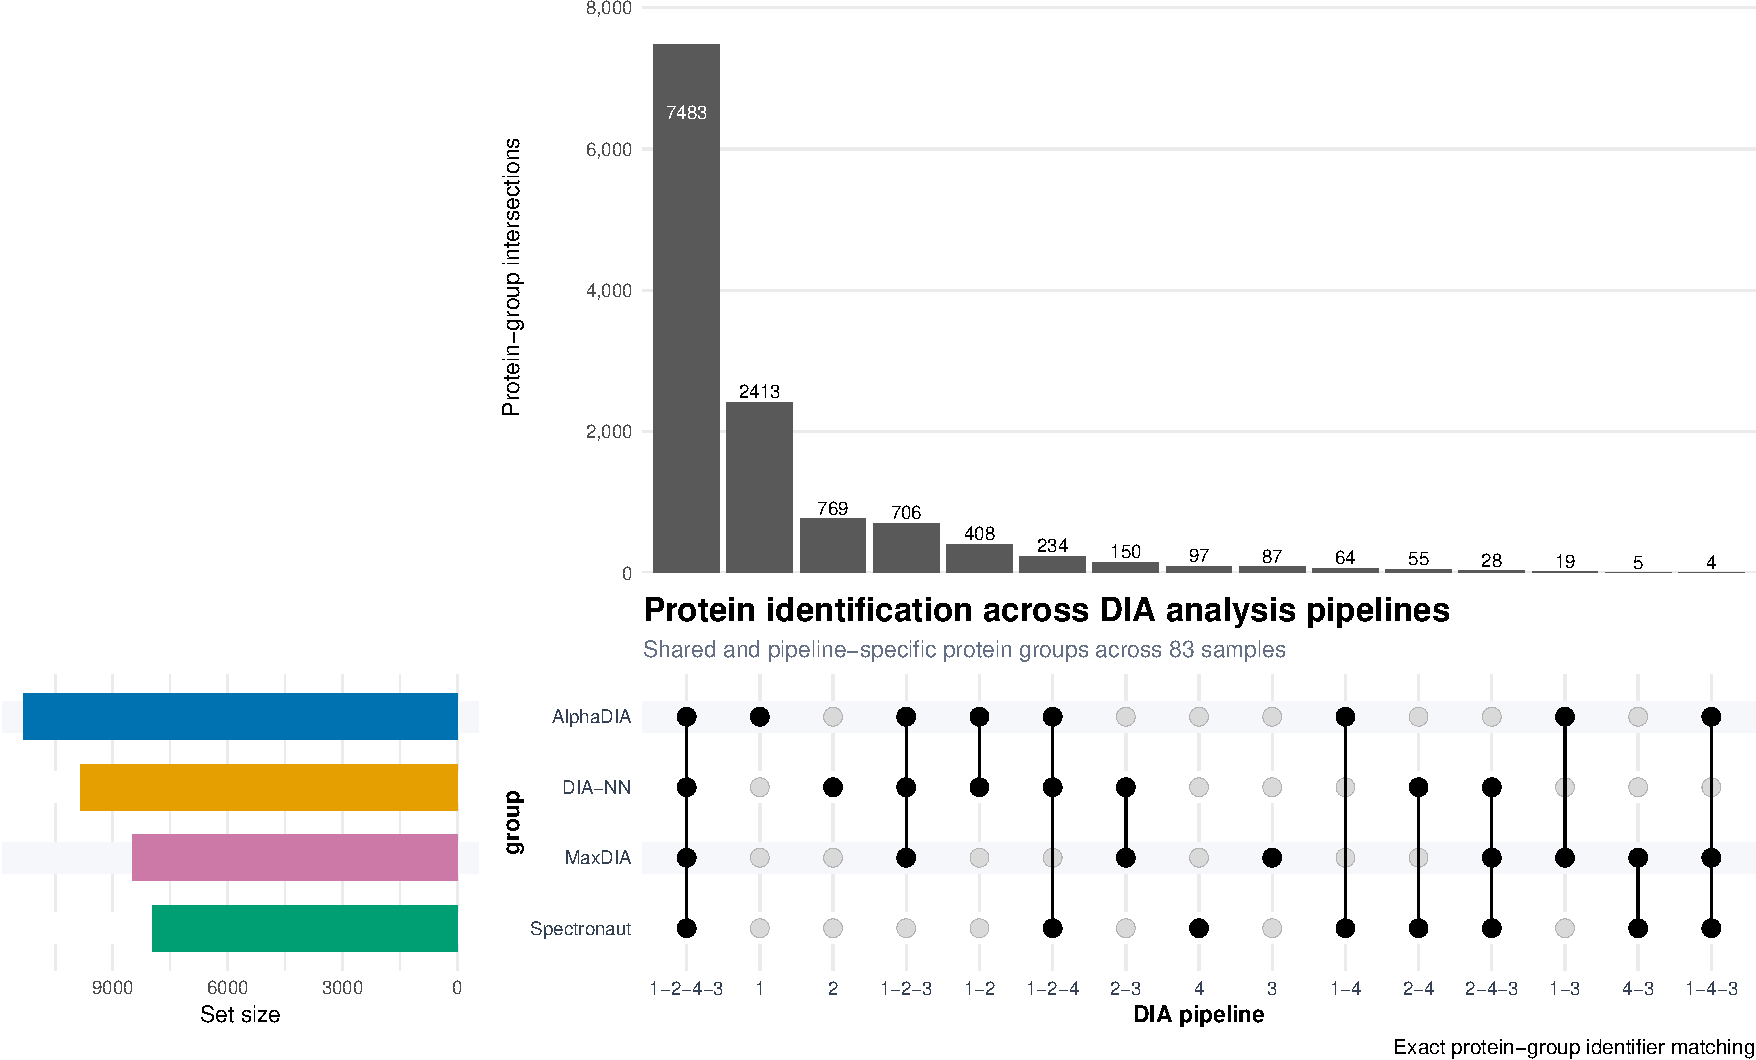
\includegraphics[width=1\linewidth]{DIA_CapstoneProject2026_files/figure-latex/upset_protein_identification-1} \end{center}

The UpSet plot shows substantial agreement in protein identification
across the four DIA analysis pipelines, with 7,483 protein groups shared
by all four tools, representing a large common proteomic core. However,
pipeline-specific differences are also evident, particularly for
AlphaDIA, which identifies the largest number of protein groups and
contributes 2,413 uniquely identified groups. DIA-NN, MaxDIA, and
Spectronaut show smaller tool-specific contributions. These findings
suggest that while the pipelines consistently identify a substantial
shared proteome, their identification coverage differs considerably.
Importantly, the overlaps are based on exact protein-group identifiers,
so differences in protein grouping between software packages may
contribute to the observed discrepancies.

\begin{verbatim}
##     Software Original_Entries Unique_Sequence_Charge Collapsed_or_Excluded
##     AlphaDIA           203024                 180846                 22178
##       DIA-NN           206959                 188855                 18104
##  Spectronaut           182083                 158701                 23382
##       MaxDIA           230167                 230167                     0
\end{verbatim}

\begin{center}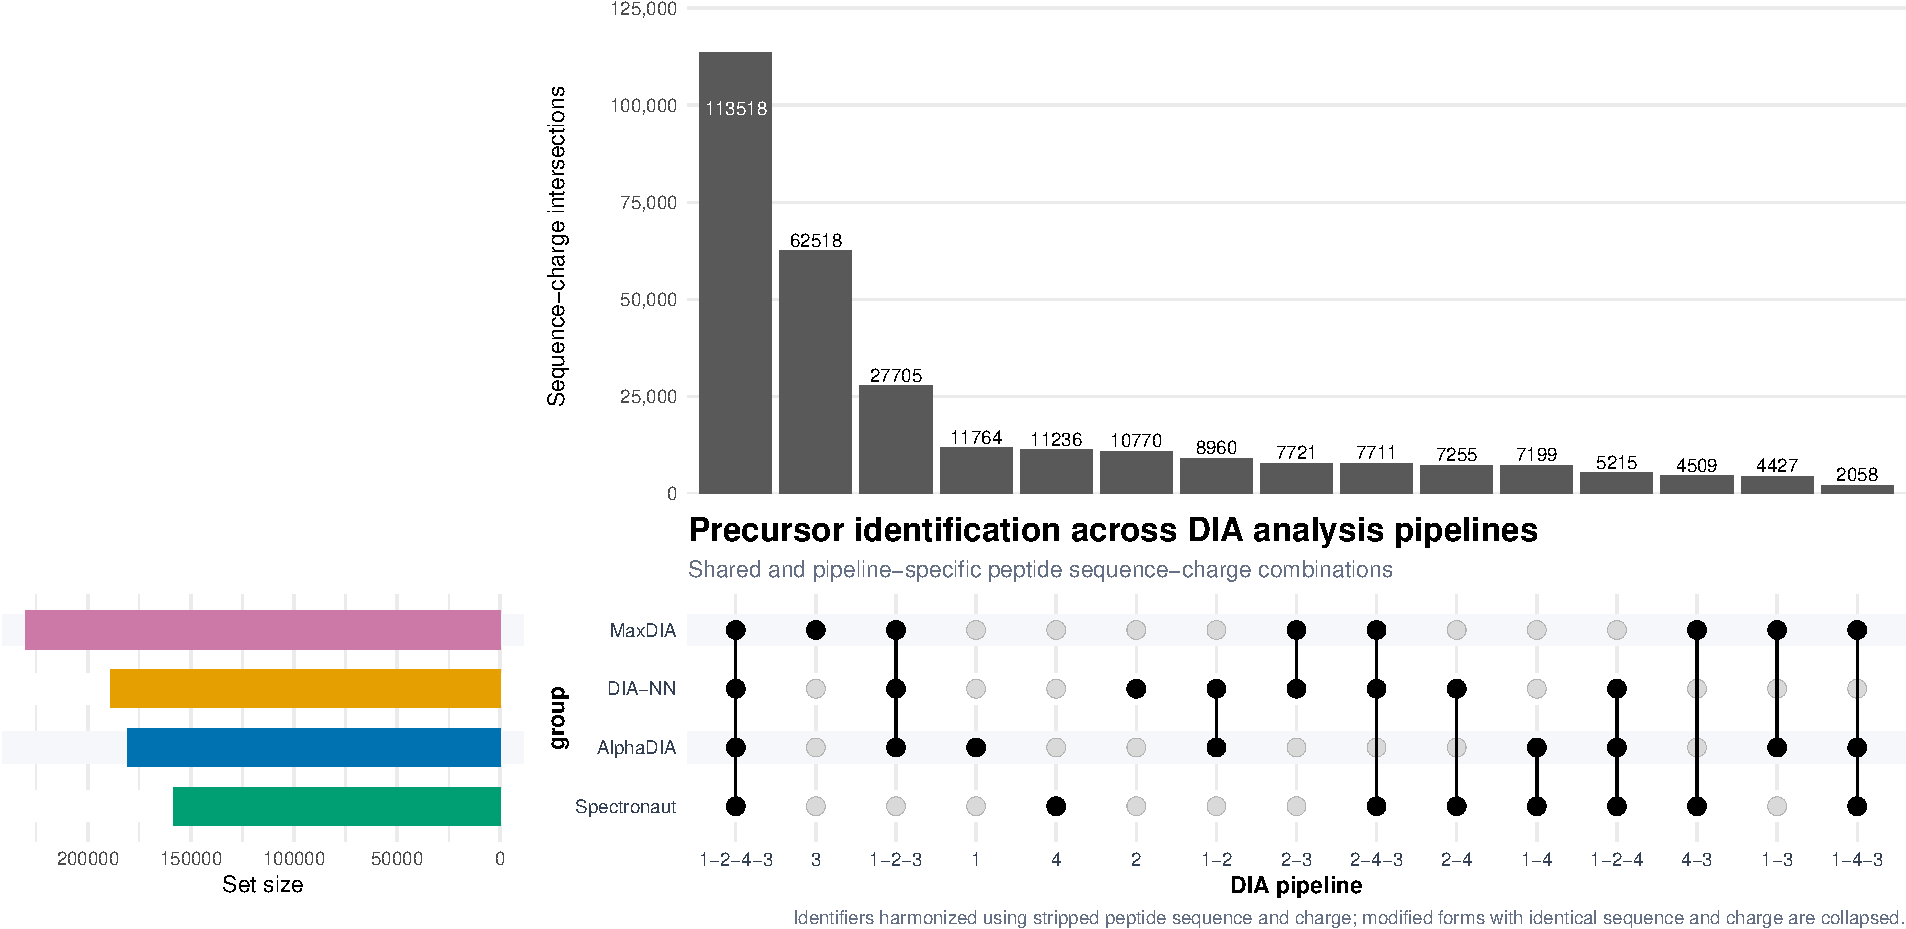
\includegraphics[width=1\linewidth]{DIA_CapstoneProject2026_files/figure-latex/upset_precursor_identification-1} \end{center}

Precursor-level identification overlap revealed a substantial shared
proteomic core across the four DIA analysis pipelines, with 113,518
peptide sequence--charge combinations identified by all four tools.
Nevertheless, considerable pipeline-specific variation was observed,
particularly for MaxDIA, which identified the largest number of unique
combinations (62,518). Spectronaut exhibited the highest proportion of
identifications belonging to the four-way intersection (71.5\%), despite
having the smallest overall sequence--charge identification set.
Compared with the protein-level analysis, these findings indicate
greater heterogeneity in precursor identification than in protein-group
coverage. This suggests that differences in precursor-level detection
and reporting may not translate directly into equivalent differences in
protein identification.

\begin{verbatim}
## # A tibble: 4 x 7
##   Software  Protein_Groups_With_~1 Mean_Precursors Median_Precursors    Q1    Q3
##   <fct>                      <int>           <dbl>             <dbl> <dbl> <dbl>
## 1 AlphaDIA                   11331            16.0                10     4    21
## 2 DIA-NN                      9833            19.2                12     5    25
## 3 Spectron~                   7970            19.9                13     5    26
## 4 MaxDIA                      8482            27.1                20    11    34
## # i abbreviated name: 1: Protein_Groups_With_Precursors
## # i 1 more variable: Max_Precursors <int>
\end{verbatim}

\begin{center}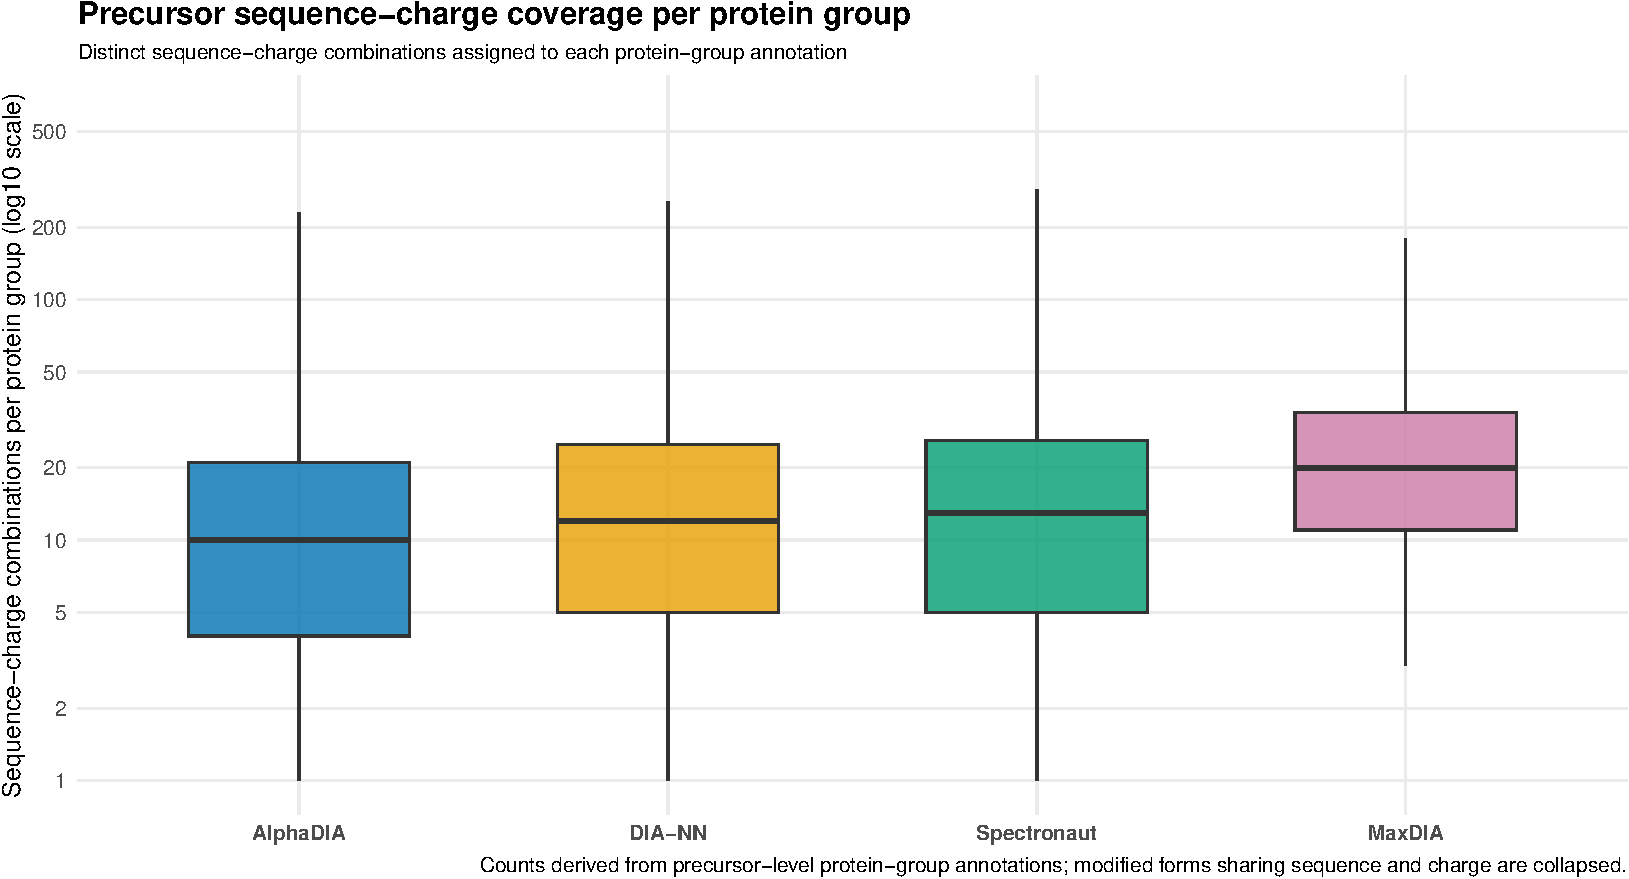
\includegraphics[width=1\linewidth]{DIA_CapstoneProject2026_files/figure-latex/precursor_coverage_per_protein-1} \end{center}

To investigate the discrepancy between MaxDIA's high precursor-level
coverage and its comparatively lower protein-group identification count,
the number of distinct peptide sequence--charge combinations assigned to
each protein group was examined. MaxDIA exhibited the highest mean
(27.1) and median (20) sequence--charge combinations per protein group,
compared with Spectronaut (19.9 and 13), DIA-NN (19.2 and 12), and
AlphaDIA (16.0 and 10), respectively. Furthermore, 99.1\% of
MaxDIA-specific sequence--charge combinations were associated with
protein accessions also identified by at least one other pipeline.
Together, these findings indicate that MaxDIA's increased
precursor-level identification coverage predominantly reflects greater
sequence--charge representation of already identified proteins rather
than a proportional expansion of protein-group coverage. Nevertheless,
differences in precursor reporting, protein inference, and filtering may
also contribute to the observed variation.

\subsubsection{Differential abundance
comparison}\label{differential-abundance-comparison}

Differential abundance analysis revealed substantial variation in the
number of significant protein groups across the four DIA pipelines and
11 experimental contrasts. AlphaDIA and DIA-NN generally reported the
largest numbers of differentially abundant proteins, whereas MaxDIA
consistently reported the fewest despite exhibiting the greatest
sequence--charge identification coverage. For example, in the KO versus
CTRL comparison following 6 hours of cisplatin treatment, DIA-NN
identified 4,021 significant proteins, compared with 3,747 for AlphaDIA,
2,709 for Spectronaut, and 647 for MaxDIA. A particularly consistent
pattern was observed for the JNK inhibitor contrasts, with all four
pipelines identifying substantially more significant proteins at 24
hours than at 6 hours. These findings demonstrate that increased
precursor-level coverage does not necessarily correspond to increased
differential abundance detection. Differences in quantitative
variability, protein inference, missingness, and statistical power may
contribute to the observed discrepancies.

Differential abundance overlap analysis for the KO versus CTRL
comparison following 6 hours of cisplatin treatment revealed substantial
agreement among the DIA pipelines, alongside differences in the number
of significant protein groups. A total of 557 protein groups were
classified as differentially abundant by all four pipelines, while 1,210
additional groups were shared by AlphaDIA, DIA-NN, and Spectronaut but
not MaxDIA. Notably, 86.1\% of MaxDIA's 647 significant protein groups
were also significant in all three other pipelines, indicating that its
smaller differential abundance set largely represented a shared subset
of findings. In contrast, AlphaDIA and DIA-NN contributed considerably
larger numbers of pipeline-specific significant protein groups. These
results demonstrate substantial cross-pipeline agreement for a common
set of differential abundance findings, while highlighting differences
in the breadth of statistically significant protein detection.

Differential abundance overlap analysis across 11 experimental contrasts
revealed a substantial shared set of significant protein groups among
AlphaDIA, DIA-NN, Spectronaut, and MaxDIA, alongside pronounced
pipeline-dependent differences. AlphaDIA and DIA-NN generally reported
the largest numbers of differentially abundant protein groups, although
their relative contributions varied across experimental comparisons.
MaxDIA consistently reported fewer significant protein groups, but a
large proportion of these overlapped with findings from the other
pipelines. For example, 557 of 647 MaxDIA-significant protein groups
(86.1\%) were significant in all four pipelines for the KO versus CTRL
comparison following 6 hours of cisplatin treatment. Similarly, four-way
intersections accounted for 644 of 871 (73.9\%) MaxDIA-significant
groups in the 24-hour JNK inhibitor comparison and 397 of 501 (79.2\%)
in the KO cisplatin 24-hour versus 6-hour comparison. Despite this
common core, substantial pipeline-specific intersections were observed,
particularly for AlphaDIA and DIA-NN. Collectively, these findings
indicate that differential abundance detection is influenced by the
analysis pipeline, with considerable agreement among shared significant
protein groups but differences in the breadth of detected responses.
Because the comparisons were based on exact protein-group identifiers
and statistical significance thresholds, further assessment of
fold-change magnitude and direction is required to establish
quantitative agreement.

\subsubsection{Pairwise log2 fold-change
comparison}\label{pairwise-log2-fold-change-comparison}

Pairwise comparison of protein-level log2 fold changes for the KO versus
CTRL contrast following 6 hours of cisplatin treatment revealed positive
quantitative agreement across all four DIA analysis pipelines, although
the strength of agreement varied. AlphaDIA and DIA-NN exhibited the
strongest concordance (Pearson r = 0.845; Spearman ρ = 0.815), with
83.0\% of shared protein groups showing consistent fold-change
directions. Comparisons involving Spectronaut demonstrated intermediate
agreement (Pearson r = 0.755--0.787), whereas MaxDIA exhibited weaker
correlations with the other pipelines (Pearson r = 0.613--0.653) and
lower directional concordance (72.4--72.9\%). These findings indicate
that differences in differential abundance detection are accompanied by
variation in estimated protein abundance changes, particularly for
MaxDIA. Although MaxDIA showed the highest precursor sequence--charge
coverage per protein group, this did not translate into greater
differential abundance detection or stronger quantitative agreement.
Further assessment of fold-change magnitude and statistical uncertainty
is needed to clarify the factors contributing to these differences.

These results are important because they challenge our earlier
hypothesis that MaxDIA detects fewer differentially abundant proteins
primarily because it estimates smaller fold changes.

Comparison of absolute protein-level log2 fold-change distributions for
the KO versus CTRL cisplatin 6h contrast showed that MaxDIA's lower
number of significant protein groups was not accompanied by uniformly
smaller estimated abundance changes. Among 7,474 protein groups with
finite fold-change estimates in all four pipelines, the median absolute
log2 fold change was 0.156 for AlphaDIA, 0.184 for DIA-NN, 0.215 for
Spectronaut, and 0.181 for MaxDIA. Spectronaut exhibited the largest
overall effect-size distribution, whereas MaxDIA showed magnitudes
broadly comparable to DIA-NN and greater than AlphaDIA. These results do
not support systematic attenuation of fold-change magnitudes as the
principal explanation for MaxDIA's reduced differential abundance
detection. Together with its weaker cross-pipeline fold-change
correlations and higher median model residual variability, the findings
suggest that differences in quantitative precision and statistical
uncertainty may contribute to the observed discrepancies. Direct
comparison of contrast-specific standard errors is required to evaluate
this explanation.

Despite comparable median absolute log2 fold changes between MaxDIA and
DIA-NN (0.181 versus 0.184) among 7,474 commonly quantified protein
groups, MaxDIA exhibited substantially higher contrast-specific standard
errors (median 0.182 versus 0.085) and lower absolute t-statistics
(median 0.951 versus 2.19). These findings suggest that reduced
statistical precision, rather than systematically smaller estimated
abundance changes, is a major contributor to MaxDIA's lower differential
abundance detection rate. The results also demonstrate that greater
precursor coverage per protein group does not necessarily translate into
greater sensitivity for detecting differential protein abundance.

MaxDIA has substantially greater protein-level residual variability than
the other three pipelines, even when we compare exactly the same 7,474
protein groups. On 7,474 matched protein groups, MaxDIA exhibited the
highest residual variability (median σ = 0.309), approximately 2.22-fold
greater than DIA-NN (0.139). This difference was accompanied by a
2.14-fold higher median standard error for the KO versus CTRL cisplatin
6h contrast, despite comparable median absolute log2 fold changes. These
findings suggest that increased residual variability, rather than
uniformly smaller estimated biological effects, contributes
substantially to MaxDIA's lower number of statistically significant
differentially abundant proteins. MaxDIA's lower differential abundance
sensitivity is associated with substantially greater residual
variability and higher statistical uncertainty, despite its greater
precursor coverage per protein.

Across all 11 differential abundance contrasts, MaxDIA consistently
exhibited the highest median standard errors and lowest median absolute
t-statistics among the four DIA analysis pipelines. This pattern
persisted when restricting each contrast to approximately 7,475 protein
groups with valid estimates in all four pipelines. MaxDIA did not
systematically produce smaller effect sizes; in seven contrasts, it
exhibited the largest median absolute log2 fold change. Combined with
its substantially higher protein-level residual variability, these
findings indicate that increased statistical uncertainty is a major
contributor to MaxDIA's lower differential abundance detection rate.

Pairwise comparison of protein-level log2 fold changes across 11
differential abundance contrasts revealed substantial differences in
agreement among DIA analysis pipelines. AlphaDIA and DIA-NN showed the
strongest overall concordance, with a median Pearson correlation of
0.719 and median directional agreement of 77.5\%. DIA-NN and Spectronaut
also exhibited relatively strong agreement (median r = 0.671). In
contrast, comparisons involving MaxDIA consistently showed lower
correlations, ranging from median r = 0.378 to 0.500, and lower
directional agreement, ranging from 63.9\% to 68.0\%. Agreement was
contrast-dependent, with stronger concordance for prominent
treatment-associated responses and weaker concordance for the JNK
inhibitor effect at 6h. Combined with MaxDIA's higher residual
variability and standard errors, these findings suggest that
pipeline-specific differences in protein quantification and statistical
precision contribute to variability in differential abundance results.
Nevertheless, cross-pipeline agreement alone cannot establish which
pipeline provides the most accurate estimates.

\subsubsection{Temporal patterns of cisplatin response and
c-Jun-dependent
regulation}\label{temporal-patterns-of-cisplatin-response-and-c-jun-dependent-regulation}

\subsection{Temporal patterns of cisplatin response and c-Jun-dependent
regulation}\label{temporal-patterns-of-cisplatin-response-and-c-jun-dependent-regulation-1}

The cisplatin response was investigated across untreated baseline,
6-hour, and 24-hour conditions in CTRL and c-Jun KO cells. Although the
existing batch-adjusted differential abundance model includes these
experimental conditions, individual pairwise contrasts do not provide a
joint test of temporal response.

We therefore examine the experimental design before evaluating overall
cisplatin-associated changes and genotype-dependent differences in
response.

\begin{verbatim}
## # A tibble: 30 x 4
##    Genotype Time     Batch        N
##    <fct>    <fct>    <fct>    <int>
##  1 CTRL     Baseline Group1       3
##  2 CTRL     Baseline Group2       3
##  3 CTRL     Baseline Group3       3
##  4 CTRL     Baseline Group4       3
##  5 CTRL     Baseline 20260331     6
##  6 CTRL     6h       Group1       0
##  7 CTRL     6h       Group2       0
##  8 CTRL     6h       Group3       3
##  9 CTRL     6h       Group4       3
## 10 CTRL     6h       20260331     0
## 11 CTRL     24h      Group1       3
## 12 CTRL     24h      Group2       3
## 13 CTRL     24h      Group3       0
## 14 CTRL     24h      Group4       0
## 15 CTRL     24h      20260331     3
## 16 KO       Baseline Group1       2
## 17 KO       Baseline Group2       3
## 18 KO       Baseline Group3       3
## 19 KO       Baseline Group4       3
## 20 KO       Baseline 20260331     6
## 21 KO       6h       Group1       0
## 22 KO       6h       Group2       0
## 23 KO       6h       Group3       3
## 24 KO       6h       Group4       3
## 25 KO       6h       20260331     0
## 26 KO       24h      Group1       3
## 27 KO       24h      Group2       3
## 28 KO       24h      Group3       0
## 29 KO       24h      Group4       0
## 30 KO       24h      20260331     6
\end{verbatim}

\begin{center}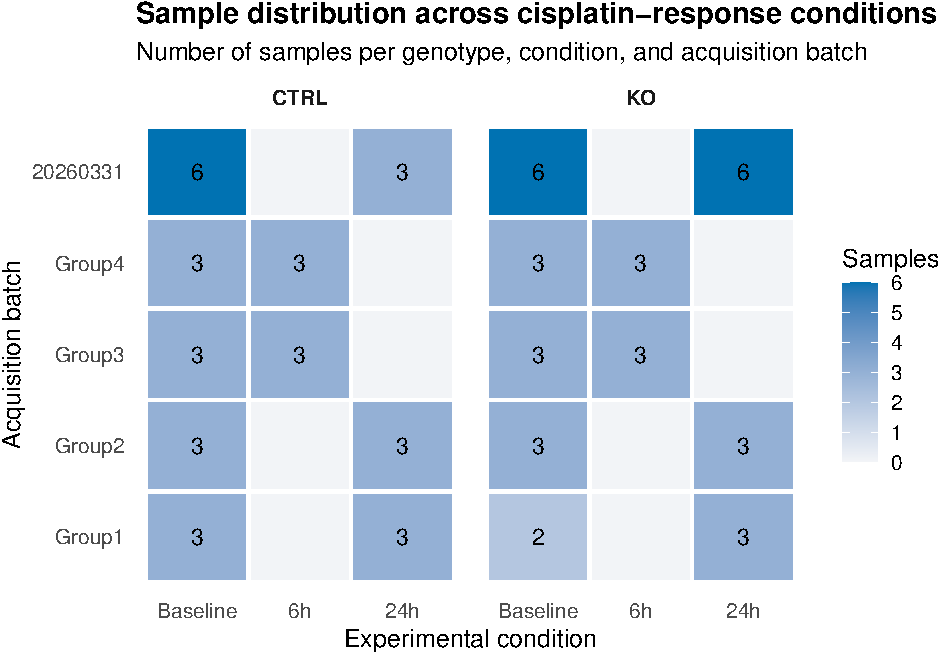
\includegraphics[width=1\linewidth]{DIA_CapstoneProject2026_files/figure-latex/temporal-design-check-1} \end{center}

These results show a clear pattern: the c-Jun KO samples exhibit a
broader cisplatin-associated proteomic response than CTRL, and all four
pipelines detect evidence of genotype-dependent responses.

\begin{enumerate}
\def\labelenumi{\arabic{enumi}.}
\tightlist
\item
  KO response is consistently more extensive than CTRL response.
\end{enumerate}

Across all four pipelines, substantially more proteins show a
significant joint cisplatin-associated response in KO than CTRL. This is
consistent with c-Jun loss being associated with altered cellular
responses to cisplatin.

However, significance counts alone do not establish that KO responses
have larger effect sizes or that every response is stronger. We would
need to examine the direction and magnitude of the individual changes.

\begin{enumerate}
\def\labelenumi{\arabic{enumi}.}
\setcounter{enumi}{1}
\tightlist
\item
  The genotype interaction is substantial.
\end{enumerate}

AlphaDIA identifies 2,820 proteins, DIA-NN 2,678, and Spectronaut 1,698
with significant joint genotype-dependent responses. MaxDIA identifies
280.

This means that, for those proteins, the KO-versus-CTRL difference in
cisplatin-associated abundance changes is statistically detectable at
6h, 24h, or both.

It does not necessarily mean that a protein responds significantly in KO
but not CTRL. The interaction directly tests the difference between the
two responses, which is the more appropriate statistical question.

\begin{enumerate}
\def\labelenumi{\arabic{enumi}.}
\setcounter{enumi}{2}
\tightlist
\item
  MaxDIA remains much less sensitive.
\end{enumerate}

Its lower discovery counts are consistent with your earlier finding of
substantially higher residual variability and contrast standard errors
in MaxDIA. The joint test has not eliminated that difference.

\begin{enumerate}
\def\labelenumi{\arabic{enumi}.}
\setcounter{enumi}{3}
\tightlist
\item
  The experimental batch structure still matters.
\end{enumerate}

The 6h and 24h cisplatin samples occupy different batches. The fitted
additive batch model adjusts for this, but interpretation relies on its
assumptions. These are cisplatin-response comparisons across
experimental conditions, not repeated measurements of the same samples
over time.

243 proteins have significant genotype-dependent cisplatin responses in
all four DIA pipelines, despite substantial differences in the total
number of discoveries. The most interesting observation is that MaxDIA
identifies only 273 significant interaction proteins among the shared
proteins, while 243 proteins are significant in all four pipelines. This
means at least 89.0\% of MaxDIA's interaction discoveries are supported
by all three other pipelines.

That suggests MaxDIA's smaller discovery set is largely a
high-confidence subset of the other pipelines' discoveries, rather than
a completely different biological signal. This is consistent with your
earlier finding that MaxDIA has higher residual variability and lower
statistical sensitivity.

One caveat: these 243 proteins agree in statistical significance, not
necessarily in the direction of their 6h and 24h interaction effects.

To investigate genotype-dependent cisplatin responses,
two-degree-of-freedom joint tests were performed using the existing
batch-adjusted, moderated protein abundance models. The tests evaluated
cisplatin-associated changes at 6 and 24 hours relative to untreated
baseline in CTRL and c-Jun KO cells, as well as differences in these
responses between genotypes.

All four DIA pipelines identified more proteins with significant
cisplatin-associated responses in c-Jun KO cells than in CTRL cells.
Significant joint genotype interactions were also detected across all
pipelines, although the number of discoveries varied substantially. When
the analysis was restricted to 7,466 proteins tested by all four
pipelines, DIA-NN identified 2,395 significant genotype interactions,
followed by AlphaDIA (2,102), Spectronaut (1,632), and MaxDIA (273). Of
these, 243 proteins were significant in all four pipelines, representing
89.0\% of MaxDIA's significant interaction proteins.

The 243 consensus proteins showed particularly strong agreement at 6
hours. All four pipelines estimated the same direction of genotype
interaction for every protein, with pairwise Pearson correlations
ranging from 0.930 to 0.982. Individual interaction testing identified
significant 6-hour effects for 243 proteins in DIA-NN and Spectronaut,
242 in AlphaDIA, and 212 in MaxDIA. In contrast, none of these consensus
proteins showed a significant individual 24-hour interaction in any
pipeline. Agreement in 24-hour effect estimates was also lower, with
49.4\% directional concordance and pairwise correlations ranging from
0.276 to 0.647.

Together, these findings indicate that the strongest cross-pipeline
consensus in genotype-dependent cisplatin responses is concentrated at 6
hours. The results also reinforce the broader benchmarking findings:
pipelines differ substantially in their ability to detect statistically
significant abundance changes, while showing strong agreement in effect
direction and magnitude for robust shared signals. Because the
experimental conditions were distributed unevenly across acquisition
batches, temporal comparisons should be interpreted as batch-adjusted
cisplatin-response contrasts rather than longitudinal measurements.

\subsubsection{Within-condition quantitative
reproducibility}\label{within-condition-quantitative-reproducibility}

\begin{verbatim}
## # A tibble: 4 x 5
##   Software    Protein_group_measurements Median_SD_log2 Q1_SD_log2 Q3_SD_log2
##   <chr>                            <int>          <dbl>      <dbl>      <dbl>
## 1 AlphaDIA                        276458          0.118     0.0637      0.213
## 2 DIA-NN                          236951          0.109     0.0583      0.204
## 3 MaxDIA                          211562          0.261     0.145       0.460
## 4 Spectronaut                     198986          0.145     0.0750      0.288
\end{verbatim}

\begin{center}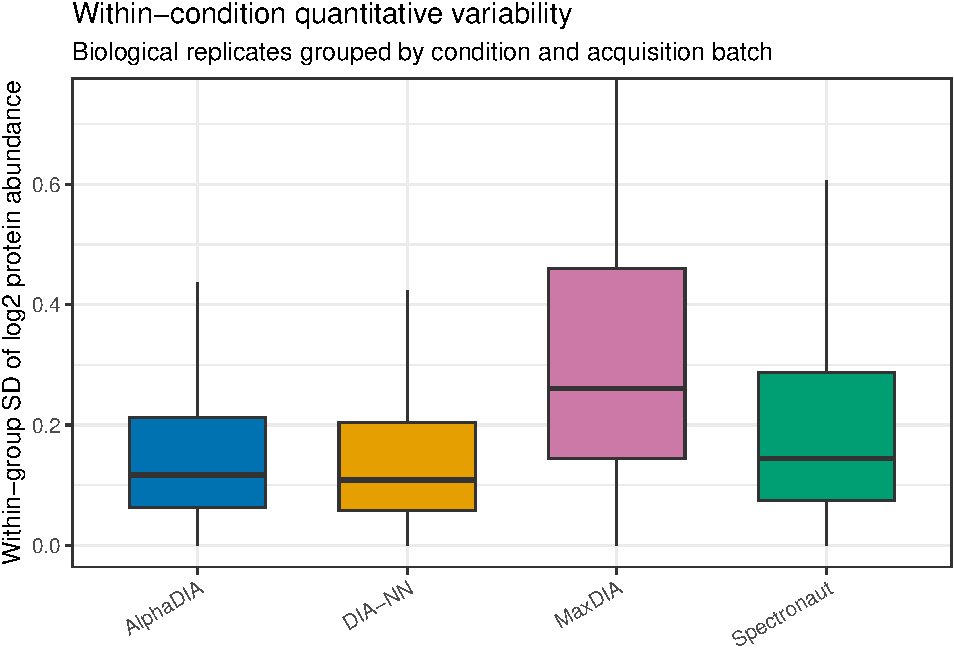
\includegraphics[width=1\linewidth]{DIA_CapstoneProject2026_files/figure-latex/within-condition-reproducibility-1} \end{center}

Within-condition quantitative variability was evaluated using the
standard deviation (SD) of log2-transformed protein abundances among
biological replicates belonging to the same experimental condition and
acquisition batch. DIA-NN exhibited the lowest median within-group SD
(0.109), closely followed by AlphaDIA (0.118), whereas Spectronaut
showed moderately higher variability (0.145). MaxDIA exhibited the
highest median SD (0.261), approximately 2.4-fold greater than DIA-NN.
The interquartile ranges followed a similar pattern, with DIA-NN
(0.058--0.204) and AlphaDIA (0.064--0.213) displaying narrower
variability distributions than Spectronaut (0.075--0.288) and MaxDIA
(0.145--0.460). These findings indicate that DIA-NN and AlphaDIA
provided the most consistent protein abundance estimates among
biological replicates, while MaxDIA showed substantially greater
within-condition variability. This observation is consistent with the
higher residual variability and lower differential abundance sensitivity
previously observed for MaxDIA. However, because the analysis included
biological rather than technical replicates and was performed on each
pipeline's quantified protein set, these results reflect combined
biological and technical variability rather than isolated technical
reproducibility.

\subsubsection{Dynamic range and abundance-dependent
precision}\label{dynamic-range-and-abundance-dependent-precision}

Abundance-dependent precision was evaluated across 7,483 proteins shared
by all four DIA pipelines by examining fitted residual standard
deviations across ten within-pipeline protein abundance deciles. All
pipelines generally exhibited decreasing residual variability with
increasing protein abundance, although the magnitude of this
relationship differed considerably. AlphaDIA and DIA-NN demonstrated
consistently low residual SDs across most abundance deciles, decreasing
from 0.218 and 0.226 in the lowest decile to 0.138 and 0.120 in the
highest decile, respectively. MaxDIA exhibited substantially higher
residual variability throughout the abundance range, with median SDs
decreasing from 0.435 to 0.296, indicating that its reduced quantitative
precision was not restricted to low-abundance proteins. Spectronaut
displayed the strongest abundance dependence, with residual SD
decreasing from 0.628 in the lowest decile to 0.147 in the highest
decile, representing a 4.27-fold difference. Although Spectronaut showed
particularly high variability among low-abundance proteins, its
precision approached that of AlphaDIA and DIA-NN at higher abundance
levels. Overall, these findings indicate that DIA-NN and AlphaDIA
maintained comparatively stable quantitative precision across the
abundance range, whereas MaxDIA exhibited consistently elevated residual
variability and Spectronaut was particularly affected at low abundance.

The pronounced abundance-dependent variability observed for Spectronaut
is consistent with the unusual low-intensity distribution identified
during initial data quality assessment, when intensity values of exactly
1 were detected and subsequently treated as missing values. Despite this
preprocessing correction, Spectronaut retained substantially elevated
residual variability among low-abundance proteins, whereas its precision
approached that of AlphaDIA and DIA-NN at higher abundance levels. This
suggests that low-abundance quantification represents a particular
limitation in the processed Spectronaut dataset, although the present
analysis cannot establish whether the original intensity-value artifact
directly contributed to the remaining variability.

\end{document}
